
\documentclass{article} % For LaTeX2e
\usepackage{iclr2025_conference,times}

% Optional math commands from https://github.com/goodfeli/dlbook_notation.
\input{math_commands.tex}

\usepackage{hyperref}
\usepackage{url}
\usepackage{floatrow}
\usepackage{graphicx}
\usepackage{amsmath}
\usepackage{amssymb}
\usepackage{mathtools}
\usepackage{amsthm}
\usepackage{mathrsfs}
\usepackage{multirow}
\usepackage[ruled,vlined]{algorithm2e}
\usepackage{enumitem}
\usepackage{amsmath}
\usepackage{tcolorbox}
\usepackage{xcolor}
\usepackage{enumitem}
\usepackage{listings}
\usepackage{multicol}
\usepackage{wasysym}
\tcbuselibrary{raster}
\lstset{
    language=Python,
    basicstyle=\ttfamily\footnotesize,
    keywordstyle=\color{blue},
    stringstyle=\color{red},
    commentstyle=\color{green!70!black},
    showstringspaces=false,
    breaklines=true,        % 自动换行
    breakatwhitespace=true,
    numberstyle=\tiny\color{gray},
}

\title{


\includegraphics[width=1.5cm]{Figures/logo1.pdf} 
\hspace{-0.5em}% 调整图片和标题文字的水平间距
AgentSquare: Automatic LLM Agent Search in Modular Design Space}

% Authors must not appear in the submitted version. They should be hidden
% as long as the \iclrfinalcopy macro remains commented out below.
% Non-anonymous submissions will be rejected without review.
\iclrfinalcopy
\author{
~Yu Shang$^{1}$\footnotemark[1]~~~~~Yu Li$^{2}$\footnotemark[1]~~~~~Keyu Zhao$^1$~~~~~Likai Ma$^1$~~~~~Jiahe Liu$^1$~~~~~Fengli Xu$^{1}$\footnotemark[2]~~~~~Yong Li$^1$\footnotemark[2]   \\
\\
~~~~~~~~~~~~~~~~~~~~~~~~~~$^1$Department of Electronic Engineering, Tsinghua University \\
~~~~~~~~~~~~~~~~~~~~~~~~~~$^2$Shenzhen International Graduate School, Tsinghua University 
}

% \author{Antiquus S.~Hippocampus, Natalia Cerebro \& Amelie P. Amygdale \thanks{ Use footnote for providing further information
% about author (webpage, alternative address)---\emph{not} for acknowledging
% funding agencies.  Funding acknowledgements go at the end of the paper.} \\
% Department of Computer Science\\
% Cranberry-Lemon University\\
% Pittsburgh, PA 15213, USA \\
% \texttt{\{hippo,brain,jen\}@cs.cranberry-lemon.edu} \\
% \And
% Ji Q. Ren \& Yevgeny LeNet \\
% Department of Computational Neuroscience \\
% University of the Witwatersrand \\
% Joburg, South Africa \\
% \texttt{\{robot,net\}@wits.ac.za} \\
% \AND
% Coauthor \\
% Affiliation \\
% Address \\
% \texttt{email}
% }

% The \author macro works with any number of authors. There are two commands
% used to separate the names and addresses of multiple authors: \And and \AND.
%
% Using \And between authors leaves it to \LaTeX{} to determine where to break
% the lines. Using \AND forces a linebreak at that point. So, if \LaTeX{}
% puts 3 of 4 authors names on the first line, and the last on the second
% line, try using \AND instead of \And before the third author name.

\newcommand{\fix}{\marginpar{FIX}}
\newcommand{\new}{\marginpar{NEW}}
\renewcommand{\thefootnote}{\fnsymbol{footnote}}
%\iclrfinalcopy % Uncomment for camera-ready version, but NOT for submission.
\begin{document}


\maketitle
\footnotetext[1]{Equal contribution.}
\footnotetext[2]{Corresponding author, correspondence to fenglixu@tsinghua.edu.cn, liyong07@tsinghua.edu.cn.}
\begin{abstract}
Recent advancements in Large Language Models (LLMs) have led to a rapid growth of agentic systems capable of handling a wide range of complex tasks. However, current research largely relies on manual, task-specific design, limiting their adaptability to novel tasks. In this paper, we introduce a new research problem: \underline{Mo}dularized \underline{L}LM \underline{A}gent \underline{S}earch (MoLAS). We propose a modular design space that abstracts existing LLM agent designs into four fundamental modules with uniform IO interface: \emph{Planning}, \emph{Reasoning}, \emph{Tool Use}, and \emph{Memory}. Building on this design space, we present a novel LLM agent search framework called AgentSquare, which introduces two core mechanisms, \emph{i.e.}, \emph{module evolution} and \emph{recombination}, to efficiently search for optimized LLM agents. To further accelerate the process, we design a performance predictor that uses in-context surrogate models to skip unpromising agent designs. Extensive experiments across six benchmarks, covering the diverse scenarios of web, embodied, tool use and game applications, show that AgentSquare substantially outperforms hand-crafted agents, achieving an average performance gain of 17.2\% against best-known human designs. Moreover, AgentSquare can generate interpretable design insights, enabling a deeper understanding of agentic architecture and its impact on task performance. We believe that the modular design space and AgentSquare search framework offer a platform for fully exploiting the potential of prior successful designs and consolidate the collective efforts of research community.
Code repo is available at \hyperlink{https://github.com/tsinghua-fib-lab/AgentSquare}{https://github.com/tsinghua-fib-lab/AgentSquare}.
\end{abstract}

\section{Introduction}

The past few years have witnessed remarkable progress in the development of Large Language Models (LLMs)~\citep{achiam2023gpt,touvron2023llama}, giving rise to the proliferation of numerous agentic systems~\citep{weng2023agent,shen2024hugginggpt}. For example, ``chain-of-thought'' prompting has unlocked the general-purpose reasoning capabilities of LLMs~\citep{wei2022chain}, and memory mechanisms have been proven effective in simulating human behavioiur~\citep{park2023generative}. These emerging LLM agents have demonstrated astonishing abilities to transform a wide range of tasks, including solving mathematical problems~\citep{romera2024mathematical}, navigating the web~\citep{nakano2021webgpt}, providing financial advice~\citep{ding2024large} and informing medical decisions~\citep{li2024agent}. Therefore, the design of agentic systems plays a crucial role in harnessing the power of LLMs for various downstream applications.

However, current research predominantly relies on manually designed agentic systems tailored for specific tasks, which often depend heavily on expert insight and intensive human labor. Furthermore, these task-specific agent designs frequently struggle to adapt to novel tasks. A few recent studies have explored using LLMs to rewrite and optimize the prompts of existing agents~\citep{fernando2024promptbreeder,yang2024large}. A more recent work introduces the idea to leverage LLMs to search the entire agentic systems defined in code space~\citep{hu2024automated}, enabling the discovery of agents with more flexible prompts, control flows, etc. 
However, these previous approaches are limited in their ability to explicitly recombine the strengths of agentic modules discovered by different researches and located in separate codebases. Another line of research focuses on optimizing the configuration of multi-agent systems~\citep{chen2023agentverse,yuan2024evoagent,li2023metaagents,zhugegptswarm,wang2023unleashing}. These efforts are orthogonal to the optimization of single-agent systems, as they focus more on the role-playing and interaction patterns among multiple agents, rather than the design of agentic modules.

\begin{figure}[!t]
\begin{center}
\vspace{-6mm}
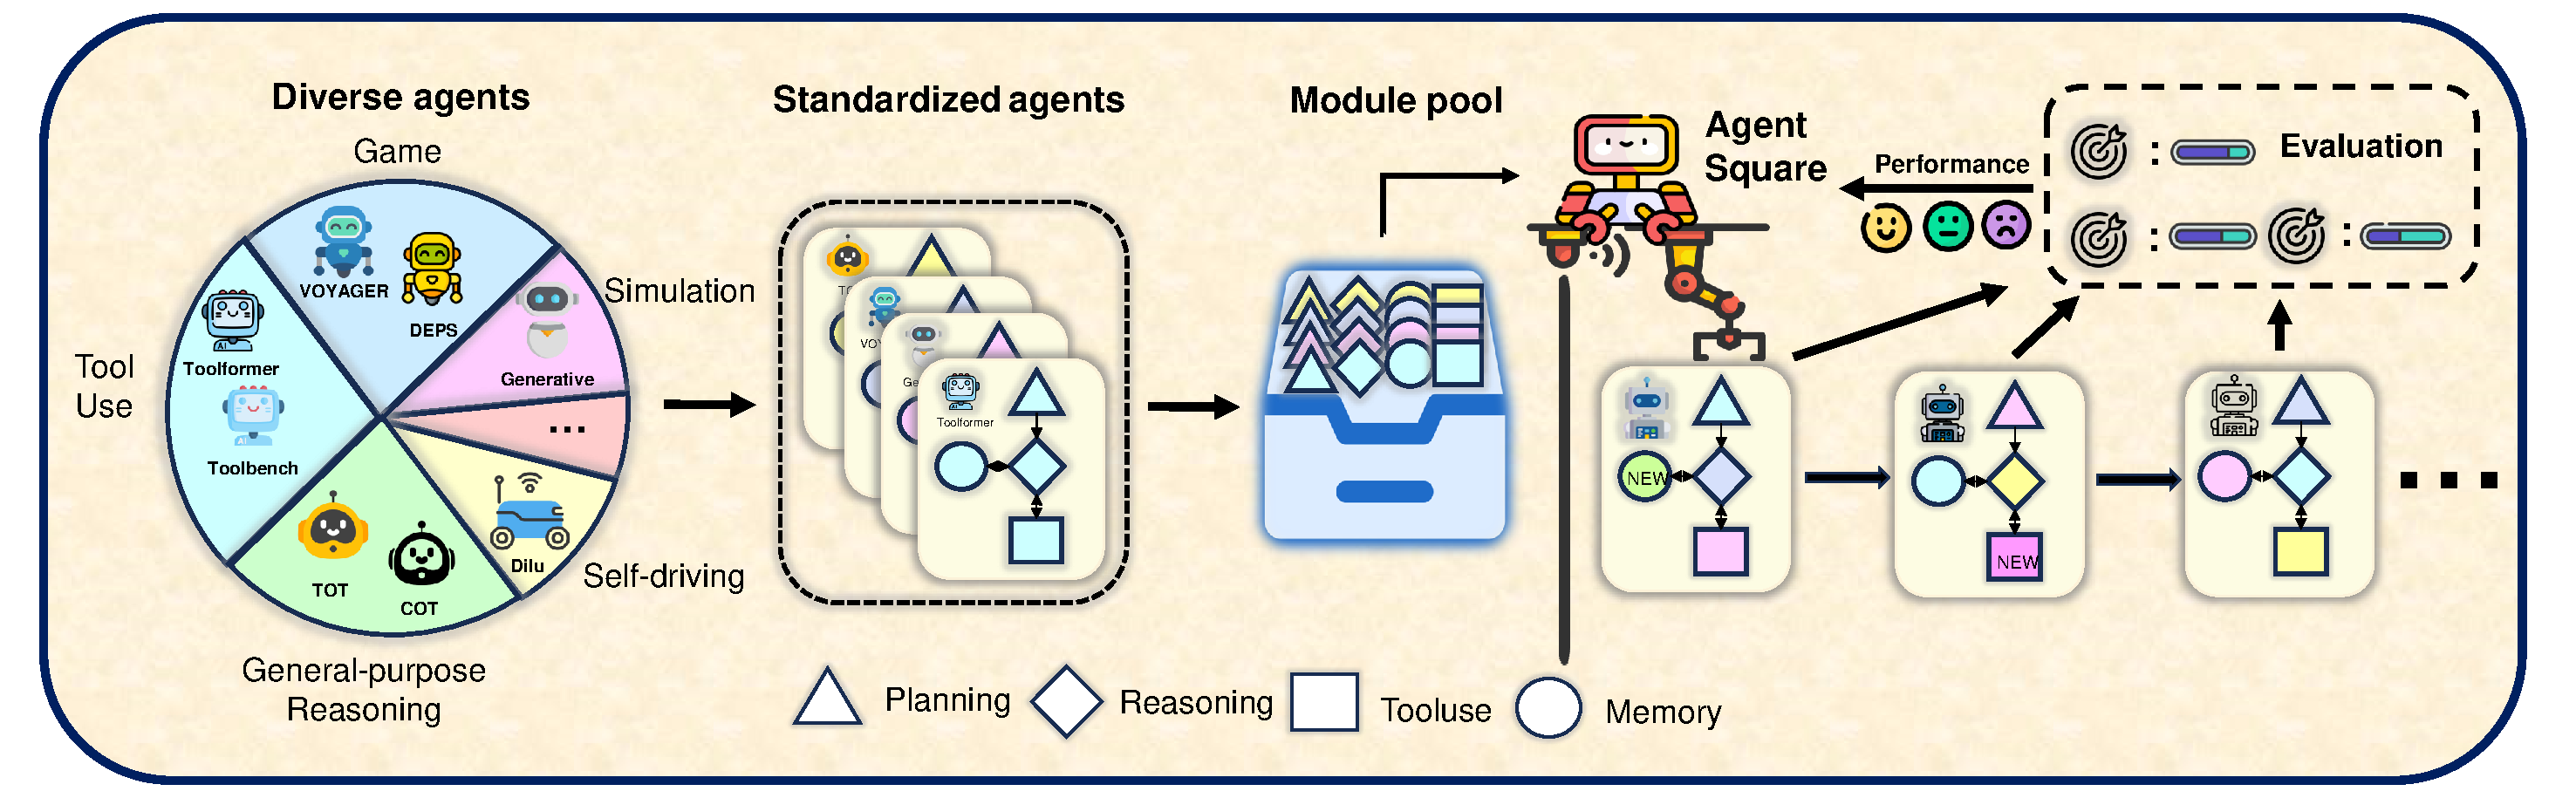
\includegraphics[width=14cm]{Figures/f1.pdf}
\vspace{-6mm}
\caption{AgentSquare is a modular framework for designing and optimizing LLM agents. 
% We first propose a modular design space of LLM agents and extract 4 types of standardized modules including planning, reasoning, tooluse, and memory. Based on this, we design a novel LLM agent search framework to automatically discover good-performing agents.
}
\label{figure1}
\end{center}
\end{figure}

This paper addresses a novel research problem --- \underline{Mo}dularized \underline{L}LM \underline{A}gent \underline{S}earch (MoLAS). The goal is to automatically optimize LLM agent designs by leveraging the experience of published or evaluated modules. Therefore, the core of our work is a modular design space for LLM agents, comprising 4 categories of modules: \emph{Planning}, \emph{Reasoning}, \emph{Tool Use}, and \emph{Memory}. This design space is abstracted from a thorough literature review of existing agentic systems (details provided in Section 2). 
% MoLAS is a guided and constrained searching problem in the modular design space, which is a subset of the entire code search proposed in ADAS. 
It is important to note that our goal is not to propose the most comprehensive, one-size-fits-all LLM agent design space, but rather to demonstrate that our modular design space enables researchers and intelligent search algorithms to fully exploit the potential of prior successful designs. 
MoLAS is a guided and constrained searching problem in the modular design space, which is a subset of the entire code search proposed in ADAS~\citep{hu2024automated}.
However, MoLAS has a nice feature of providing standardized IO interfaces for agent modules, facilitating easy recombination of modules from different agentic systems and hence enabling efficient search for novel agents. Our design space is also highly extensible, allowing new agentic systems to be integrated as plug-in modules. Therefore, it provides a platform to consolidate the collective efforts of the research community on LLM agents. The overview of this work is illustrated in Figure~\ref{figure1}.

Building on this modular design space, we propose a novel LLM agent search framework called AgentSquare. Specifically, AgentSquare optimizes LLM agents through the mechanisms of \emph{module evolution} and \emph{recombination}. The \emph{module evolution} mechanism leverages an evolutionary meta-prompt to explore new modules through prompt-level optimization, which jointly models task descriptions, existing modules, and the performance of evaluated modules. Besides, the \emph{module recombination} mechanism performs module-level optimization by leveraging the reasoning power of LLMs to strategically search for promising module combinations. To reduce the expensive evaluation costs of LLM agents, we further introduce a performance predictor that implements an in-context surrogate model for newly proposed LLM agents, enabling us to skip unpromising candidates and significantly accelerate the search process.

We conduct comprehensive evaluations on six widely adopted benchmarks, covering diverse use cases in web, embodied, tool use and game scenarios. Our experiments show AgentSqaure can discover novel LLM agents that outperform hand-crafted agents across all six benchmarks, scoring an average performance gain of 17.2\% compared to the best known human designs. Besides, AgentSqaure also surpasses other search algorithms in terms of having a steeper optimization trajectory. More importantly, case studies reveal that AgentSquare can provide human interpretable design insights for newly discovered, good-performing agents.

The key contributions of this work are as follows:

\begin{itemize}
    \item We propose a novel modular design space for LLM agents, enabling researchers to easily build on previous successful designs and accumulate new discoveries as a community.
    \item We design the AgentSquare framework that efficiently searches for novel and good-performing LLM agents via the novel mechanism of \emph{module evolution}, \emph{module recombination}, and \emph{performance predictor}.  
    \item Experiments across six diverse tasks show that our method discovers novel LLM agents that outperform all known human designs. Besides, AgentSqaure can generate human interpretable design insights for these novel agents. 
\end{itemize}


\section{A Modular Design Space of LLM Agents}

\begin{figure}[!t]
\vspace{-6.5mm}
\begin{center}
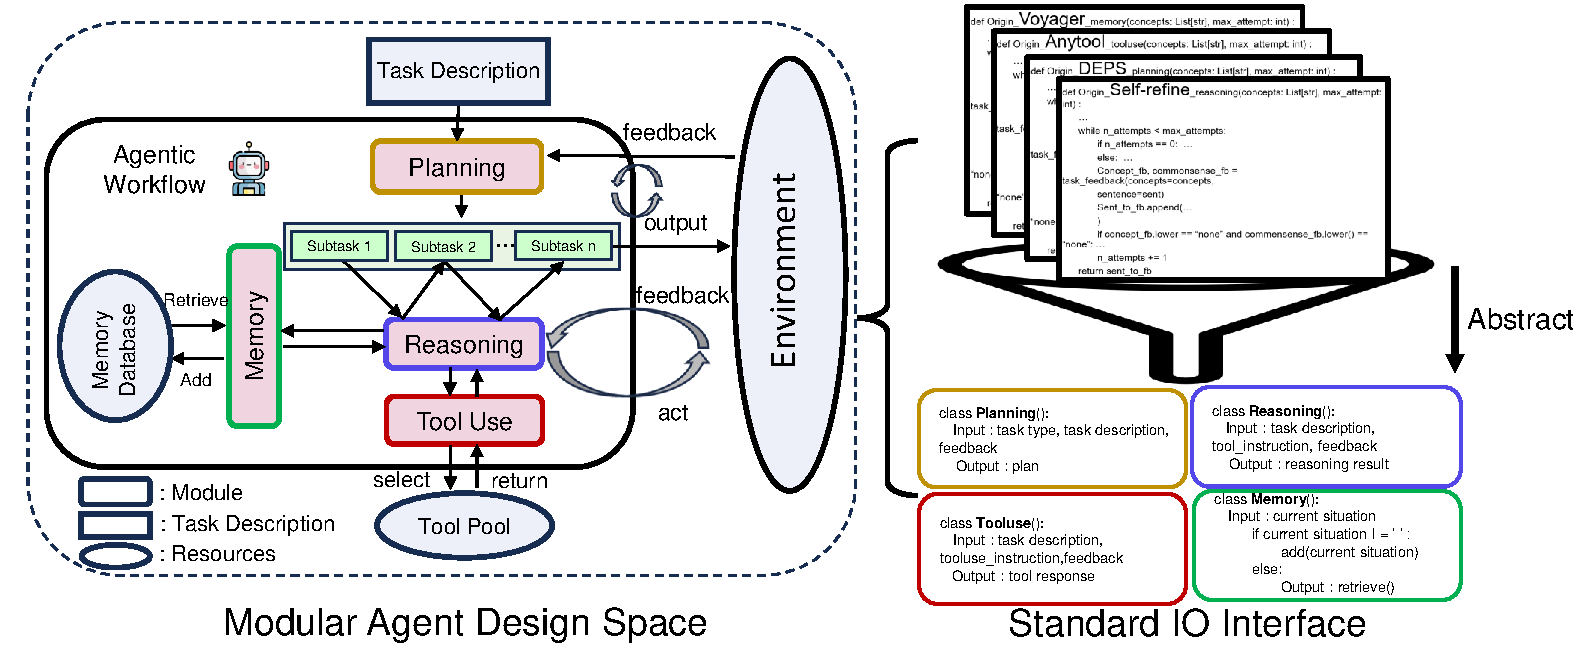
\includegraphics[width=14cm]{Figures/f2.pdf}
\caption{Illustration of the modular agent design space and agentic workflow (left) and the standardized IO interface of four types of modules (right).}
\label{figure2}
\end{center}
\end{figure}

\subsection{Background}

Using LLMs for automatic optimization has been a widely explored topic, such as applications in code generation~\citep{lehman2023evolution,romera2024mathematical} and neural architecture search~\citep{nasir2024llmatic,chen2024evoprompting}.
There are several recent studies that explore the problem of prompting LLMs to design LLM agentic systems. OPRO~\citep{yang2024large} and Promptbreeder~\citep{fernando2024promptbreeder} can be viewed as leveraging the reasoning power of LLMs to improve the prompt of LLM agents. More importantly, ADAS introduces the idea of searching the entire agentic system defined in code space, and propose a Meta Agent Search algorithm that discovers LLM agents outperforming state-of-the-art human designs~\citep{hu2024automated}. Our main difference and contribution lie in introducing a modular design space for LLM agents, which can provide a standard framework to support the convenient reuse of existing successful agent components and fruitful innovative agent module discovery. 

A modular design space for LLM agents facilitates the reuse of prior successful designs and supports the exploration of new architectures. 
At the core of such modularization is the standardization of input-output interfaces, which ensures both extensibility and seamless integration with existing designs.
Many experts in the field have proposed building LLM agentic systems with key modular components from engineering~\citep{weng2023agent} and cognitive perspectives~\citep{sumers2023cognitive}. 
However, these proposals remain largely conceptual, lacking implementable solutions to unify existing LLM agents. Besides, current LLM workflow program frameworks (\emph{e.g.}, LangChain and AutoGPT) only provide operation-level components, which cannot support module-level search that best exploits the potential of prior successful designs.

To address these problems, we perform a comprehensive literature review of publications from NeurIPS, ICML, and ICLR over the past three years. 
The review focuses on papers with the keywords ``LLM'', ``Agent'', or ``Large Language Model'' in their titles while excluding works related to multi-agent systems or agents that require additional training.
Note that our aim is not to propose the most comprehensive, one-for-all LLM agent design space, but to offer a standardized framework that enables the recombination of existing agents and facilitates the discovery of new ones.
As a result, we sort out 16 popular LLM agents and abstract a modular design space with 1050 possible combinations, which can be easily extended when new modules are discovered.
Below, we describe the agentic workflow and the function of four modules in our design space.

\subsection{Workflow overview}
The proposed agent workflow operates through an iterative process with the interconnection of the above four modules, as shown in Figure~\ref{figure2}. 
Upon receiving a task $d$, the agent starts with the \emph{planning} module, decomposing it into $n$ sub-tasks$\{s_1, s_2, \dots, s_n\}$. 
Next, these sub-tasks are passed to the \emph{reasoning} module sequentially.
Taking the sub-task $s_i$ description as input, the \emph{reasoning} module explores to prompt LLMs to give the result.
When reasoning encounters limitations in internal knowledge of LLMs, the \emph{tool use} module is activated to select an appropriate tool from the pre-defined tool pool $\tau$, supporting problem-solving.
Besides, the reasoning process also accesses the \emph{memory} module which reads and writes necessary observations and experiences from a memory database $mem$ to help reasoning.
The reasoning result of each sub-task will be transformed into actions, guiding the agent to interact with the external environment.
% Combined with the received feedback from the environment, the \emph{reasoning} module runs iteratively to refine the reasoning results.
After all sub-tasks are finished or the reasoning process gets stacked, the agent will activate the \emph{planning} module to adjust the plan with the received feedback.
The agent conducts such a trial-and-error loop until the task $d$ is completed or the set maximum trial number is reached.

\textbf{Planning.} 
The planning module is responsible for decomposing the targeted task into smaller sub-tasks. 
Given a task description $d$ and optional feedback information $f$, the planning module $P$ strategically decomposes the targeted task into a sub-task sequence $ \{s_1, s_2, \dots, s_n\} = P(d, f)$.
Such decomposition is critical for handling very complex tasks with long-term characteristics, especially for agents in open-world environments such as MineCraft~\citep{wang2024voyager,wang2024describe}.

\textbf{Reasoning.}
LLMs have exhibited remarkable reasoning abilities under advanced prompting approaches such as CoT~\citep{wei2022chain}, ToT~\citep{yao2024tree}, and SoT~\citep{shang2024defint}, shaping the foundation of the intelligence of LLM agents.
The reasoning module $R$ is invoked to solve the sub-tasks sequentially after planning, which takes each sub-task $s_i$ and optional feedback information $f_i$ as input and outputs a solution $r_i=R(s_i,f_i)$.
% This is usually achieved by diverse prompting approaches for LLMs, such as Chain-of-Thought (CoT) and Tree-of-Thoughts (ToT).

\textbf{Tool use.}
The ability of using external tools~\citep{shen2024hugginggpt,schick2024toolformer} overcomes the limitations of the LLM’s internal knowledge during the reasoning process. 
% This module is designed around \textit{when} to use tools and \textit{how} to select the most appropriate tool. 
% When the reasoning process needs external assistance, the tool use module $T$ will be invoked to select the suitable tool for problem-solving.
Formally, given certain problem $p_{ij}$ derived from the reasoning process of sub-task $s_i$ and a pre-defined tool pool $\tau$, the tooluse module $T$ selects the best-matched tool $t_{ij}$ to address the problem, denoted as $t_{ij} = T(p_{ij}, \tau)$, where $t_{ij} \in \tau$. 

\textbf{Memory.}
Memory plays a critical role by storing past thoughts, actions, and observations of agents~\citep{park2023generative,shinn2024reflexion}.
% These internal logs are dynamically written to and retrieved from the memory, controlled by a reflection module.
During the reasoning process, these internal logs are dynamically written to and retrieved from the memory database $mem$, controlled by the memory module $M$.
The writing process can be expressed as $mem = M_{write}(o, mem)$, where $o$ denotes the current observations. The retrieval process is $m = M_{retrieve}(o, mem)$, where $m$ denotes the retrieved knowledge relevant to the current situation.



\section{AgentSquare Framework}

\begin{figure}[!t]
\begin{center}
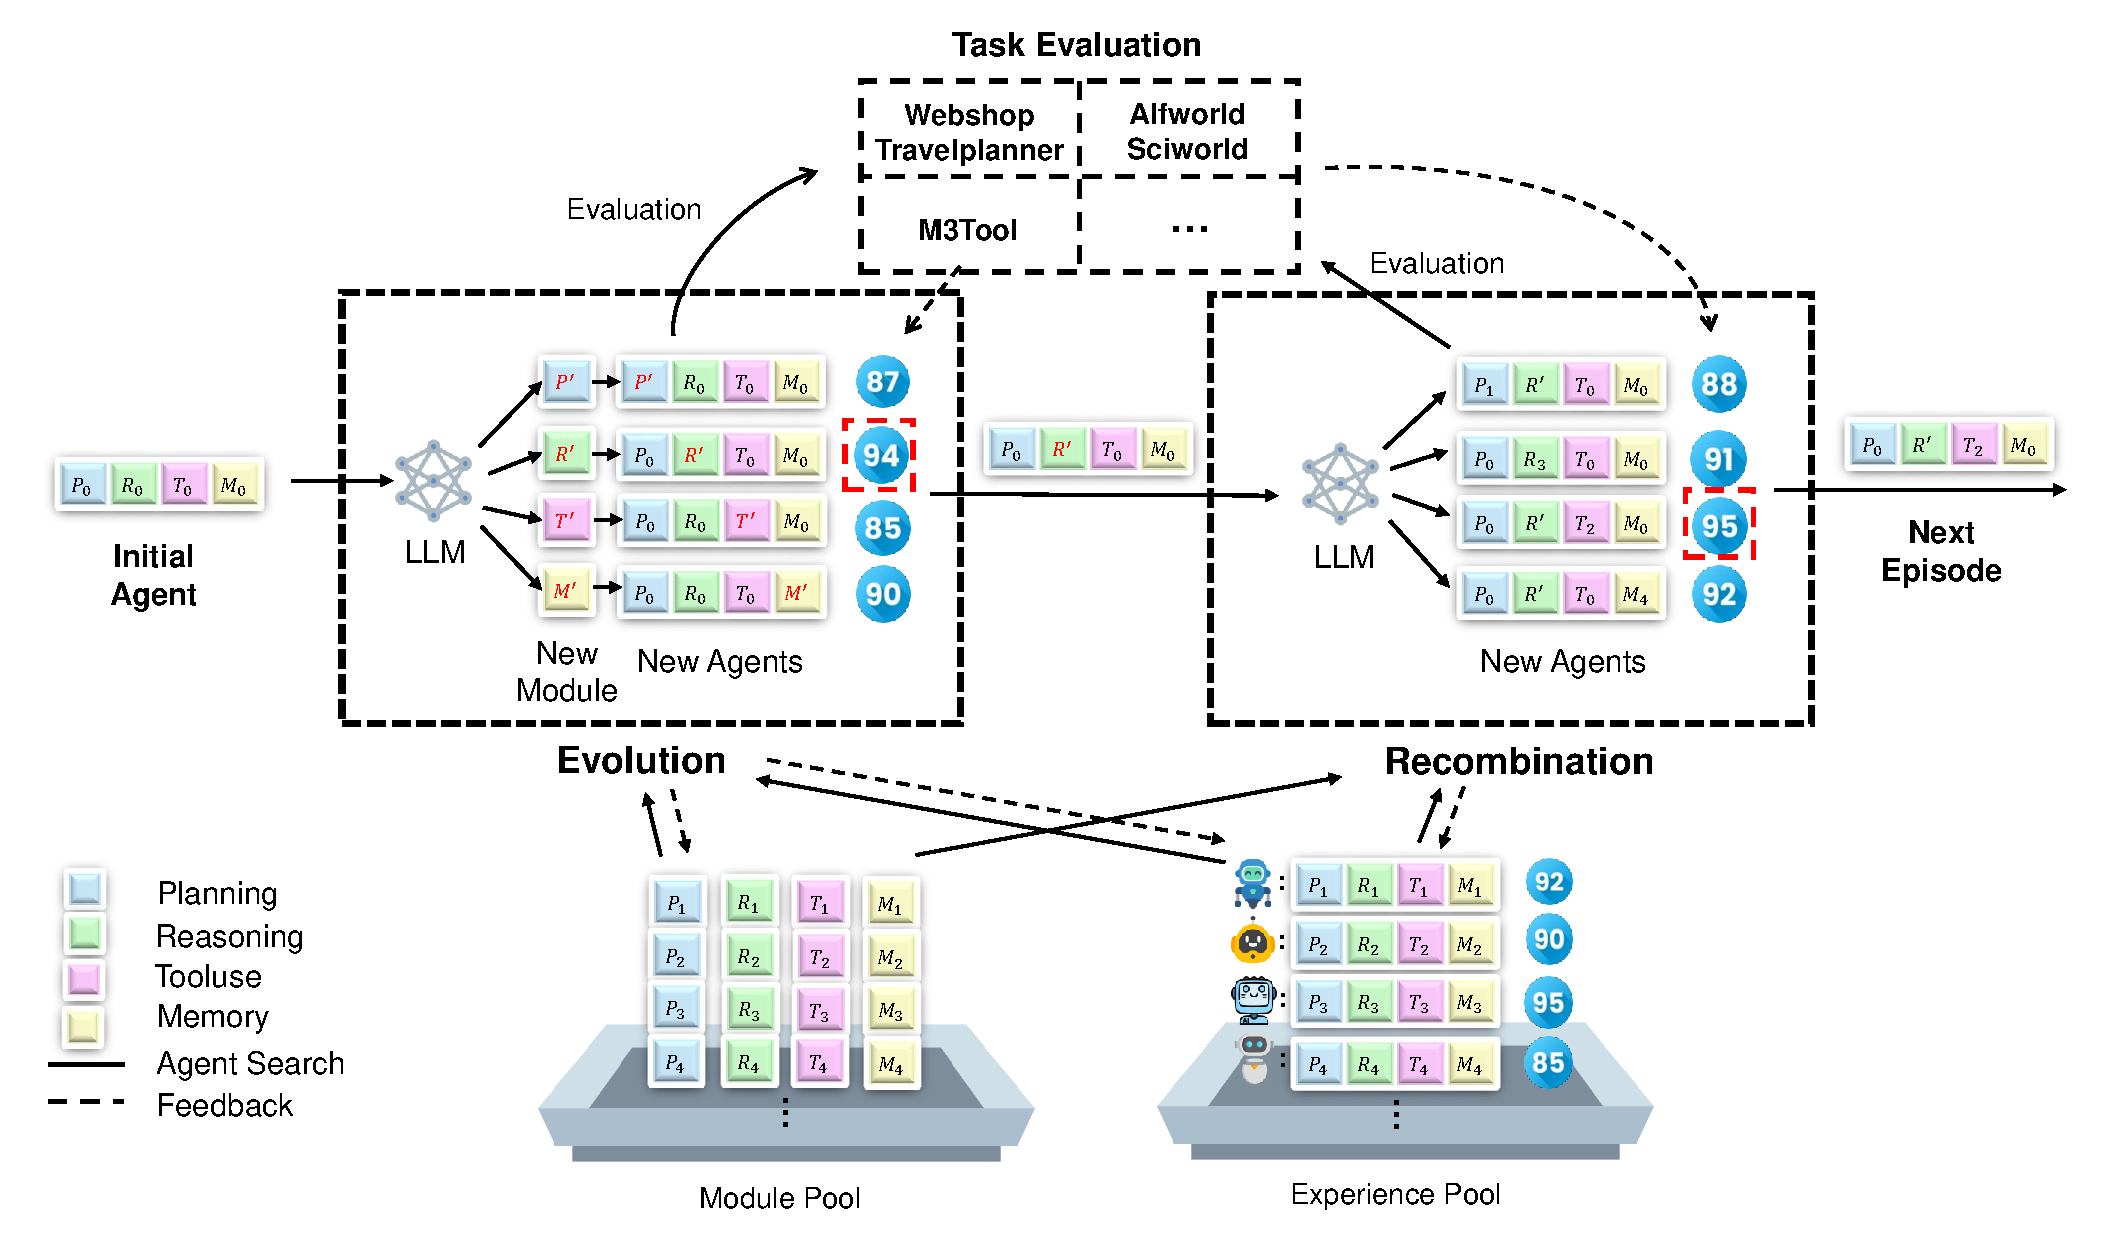
\includegraphics[width=12cm]{Figures/f3.pdf}
\caption{Overview of AgentSquare search framework. AgentSquare optimizes LLM agents through the mechanisms of module evolution and recombination. We further introduce a performance predictor that implements an in-
context surrogate model for efficient evaluation of novel agents.}
\label{framework}
\end{center}
\end{figure}
\subsection{Problem formulation of MoLAS}
In the proposed modular design space, an LLM agent $A$ can be instantiated with the combination of a planning module $P$, a reasoning module $R$, a tooluse module $T$ and a memory module $M$, denoted as $A = (P, R, T, M)$.
Given the task description $d$ and the set of all possible modules with standardized IO interface $\{\mathbb{P}, \mathbb{R}, \mathbb{T}, \mathbb{M}\}$.
We formulate an optimization problem for searching LLM agent architectures within the modular design space. 
The objective is to identify the optimal module combination in a solution space defined by a Cartesian product of four design dimensions to maximize agent performance.
Let the performance evaluation function of the task be ${Eval}_d(\cdot)$, where the specific metric varies in different tasks as discussed in Appendix~\ref{app:setup}. The optimization problem of MoLAS is defined as follows:
\begin{equation}
    \argmax\limits_{ P \in \mathbb{P}, R \in \mathbb{R}, T \in \mathbb{T}, M \in \mathbb{M}} {Eval}_d(P,R,T,M).
\end{equation}

\subsection{AgentSquare search algorithm}
Solving the optimization problem of MoLAS features three key challenges: (1) The search space, defined as the Cartesian product of four orthogonal modules, is vast and hard to explore;
(2) the module sets encompass any code with standard IO interfaces, making the module selection an open-ended problem; (3) the high costs of agent evaluation during the search process constrain the overall search scale.
To tackle these issues, we introduce AgentSquare, an automatic search framework to optimize LLM agents within the modular design space. 
Facing the vast search space of MoLAS, we propose \emph{module recombination} operation utilizing LLMs to strategically reason to identify more promising module combinations.
Such operation broadens the coverage of child samples, overcoming the limitations of prompt rewrite methods that explore only a restricted space.
However, only searching in the existing module combinations also narrows the search space, thus we propose \emph{module evolution} operation which employs an evolutionary meta-prompt to search new modules through code-level optimization.
This operation, combined with module recombination, enables the search of any module combination in the open-ended solution space.
Finally, to mitigate the high costs of frequent evaluations of searched agents, we design a \emph{performance predictor} as an in-context surrogate model for evaluating searched agents, significantly accelerating the search process and reducing real-valued costs.
% AgentSquare introduces three key designs for efficient agent optimization: \emph{module evolution}, which  \emph{module recombination}, which strategically switches certain modules with existing ones from standardized module pools, and \emph{performance predictor}, utilizing LLM to provide cost-efficient agent evaluation during search processes.

% In each search episode, AgentSquare optimizes an initial agent through alternating module evolution and recombination operations. 
% It starts with a module evolution phase programming new modules in code format.
% These newly created modules are individually integrated into the current agent, producing several child agents. 
% Each child agent is then evaluated, and the best-performing one is selected as the initial agent for the subsequent module recombination phase.
% During the recombination phase, AgentSquare utilizes an LLM to strategically replace certain modules with others from the standardized module pool.
% The generated agents are then evaluated, and the best one is selected as the initial agent in the next episode.
% Such search process is ended when it's unable to generate better agents or a predefined maximum number of search episodes $K$ is reached.
The overall framework of AgentSquare is illustrated in Figure~\ref{framework} and the algorithm is presented in Algorithm~\ref{alg}. 
Next, we detail the key components of the AgentSquare search process.

% \begin{algorithm}[t!] 
% % \SetAlgoNoLine 
% \caption{Algorithm of AgentSquare} 
% \label{alg}
% % \LinesNumbered 
% \KwIn{
% Initial agent $A_0$, targeted task descriptions $d$, maximum evolution episode $K$,  population size $N$ per evolution phase, standardized module pools $\{\mathbb{P}, \mathbb{R}, \mathbb{T}, \mathbb{M}\}$, experience pool $\mathbb{E}$ 
% }
% \KwOut{The evolved agent $A^*$}
% $t \leftarrow 1$ \tcp{Current search episode}
% $A_e^0 \leftarrow A_0$  \tcp{Initialization of the module evolution phase} 
% \While{$t \leq K$}{
% $\{A_e^1,A_e^2,...,A_e^N\} \leftarrow \pi_{\xi} (A_e^0, d, N, \mathbb{P}, \mathbb{R}, \mathbb{T}, \mathbb{M}, \mathbb{E})$ 
% \tcp{Module evolution}
% $A_r^0 \leftarrow \argmax\{{Eval}_d(A_e^0), {Eval}_d(A_e^1),...,{Eval}_d(A_e^N)\}$  \tcp{Select the best-performing generated agent} \\
% $\{A_r^1,A_r^2,...,A_r^N\} \leftarrow \pi_{\theta} (A_r^0, d, N, \mathbb{P}, \mathbb{R}, \mathbb{T}, \mathbb{M}, \mathbb{E})$ \tcp{Module recombination} \\
% $A_e^0 \leftarrow \argmax\{{Eval}_d(A_r^0), {Eval}_d(A_r^1),...,{Eval}_d(A_r^N)\}$ \tcp{Select the best-performing generated agent} \\
% $ t \leftarrow t+1$ 
% }

% $A^* \leftarrow A_e^0$ 

% \Return $A^*$
% \end{algorithm}

\subsection{Initialization}
Insights from existing AutoML studies indicate that a well-chosen initialization enhances warm-up and improves search efficiency by avoiding unpromising populations~\citep{so2019evolved,yuan2024evoagent}.
AgentSquare starts by initializing a global experience pool $\mathbb{E} = \{(P,R,T,M,v)|P_0 \in \mathbb{P}, R_0 \in \mathbb{R}, T_0 \in \mathbb{T}, M_0 \in \mathbb{M}\}$ to seed agents that are well-designed (as mentioned in Section 2) along with their real-valued performance $v$.
The module pools $\{\mathbb{P},\mathbb{R},\mathbb{T},\mathbb{M}\}$ are set to the standardized modules extracted from these seed agents.

\subsection{Module Recombination}
% Denote the initial agent in the module evolution phase as $A_e^0 = (P_0, R_0, T_0, M_0)$, where $P_0 \in \mathbb{P}, R_0 \in \mathbb{R}, T_0 \in \mathbb{T}, M_0 \in \mathbb{M}$. 
% represents the planning, reasoning, tooluse and memory module from corresponding standardized module pools.
Given the vast solution space of MoLAS, relying solely on prompt rewriting leads to a limited exploration confined to the neighbor of the initial state.
To expand the exploration space, we propose leveraging LLMs as a \emph{self-adaptive proposer}, which iteratively reason to identify promising module combinations with accumulated experience beyond the original agent configuration.
Denote the initial agent of the recombination phase as $A_r^0 = (P_0,R_0,T_0,M_0)$, where $P_0 \in \mathbb{P}, R_0 \in \mathbb{R}, T_0 \in \mathbb{T}, M_0 \in \mathbb{M}$.
The module combination proposer LLM $\pi_{\theta}$ incorporates targeted task description $d$, existing module pools $\{\mathbb{P}, \mathbb{R}, \mathbb{T}, \mathbb{M}\}$ and the performance experience of searched module combinations $\mathbb{E}$ to propose promising new agents $A_r$:
\begin{equation}
    A_r = \pi_{\theta}((P_0,R_0,T_0,M_0), d, N, \mathbb{P}, \mathbb{R}, \mathbb{T}, \mathbb{M}, \mathbb{E}).
\end{equation}

% The module evolution operation focuses on exploring novel modules to evolve agents, while the recombination operation aims to exploit existing modules to construct new agents.
% Denote the input agent of the recombination phase as $A_r^0 = (P^{'}_0,R^{'}_0,T^{'}_0,M^{'}_0)$, where $P^{'}_0 \in \mathbb{P}, R^{'}_0 \in \mathbb{R}, T^{'}_0 \in \mathbb{T}, M^{'}_0 \in \mathbb{M}$.
% The recombination operation leverages an LLM to strategically replace certain modules of the current agents with other existing modules, considering module profiles, targeted task descriptions, and performance experience of tested module combinations.
% The meta-prompt used for module recombination is presented in Figure~\ref{app:module-level1}.
Based on the initial agent configuration $A_r^0$, the LLM proposes $N$ offspring $\{A_r^1,A_r^2,...,A_r^N\}$ by replacing certain modules of $A_r^0$ with alternatives from the module pool. 
For instance, a possible solution could be $(P_0,R^{'},T_0,M_0)$, where $R^{'} \in \mathbb{R}$ is a different reasoning module selected from the module pool.
% Given the high cost of evaluating each generated agent in the task environment, here we introduce a cost-efficient agent performance predictor for agent evaluation.
% Specifically, we design a meta-prompt incorporating module profiles, targeted task descriptions, and performance history of previously tested agents for an LLM to predict the performance of newly generated agents.
% We have observed a strong correlation between the predicted and the agents' actual performance, showing the effectiveness of the performance predictor. 
% The results are presented in Figure X in the experimental section.
Then, the created $N$ new agents are evaluated with a performance predictor $\pi_p$ (detail in Seciton~\ref{section:pp}) and the best one goes to the next episode as initialization.

\subsection{Module Evolution}
As mentioned above, the solution space for each module type is open-ended, allowing any code with a standardized I/O interface. 
Consequently, searching only with module recombination narrows the solution space and limits the upper bound of agent performance.
To address this problem, we design a \emph{module evolution} operation with an evolutionary meta-prompt to search for new modules through program-level optimization.
This design is inspired by the iterative pipeline of FunSearch~\citep{romera2024mathematical}, which prompts LLMs to propose new solutions based on the target problem and performance feedback from existing solutions. 
Building on this concept, we introduce a module-programming LLM $\pi_{\xi}$ to conduct agent search in our modular design space by jointly modeling task descriptions, existing modules, and the performance of previously evaluated modules. Please note we reuse parts of the open-source code from ADAS~\citep{hu2024automated} to implement the optimization procedure.
Leveraging LLMs to search in the modular agent design space has several appealing advantages. 
Compared with the unconstrained design space of LLM agents, searching functional modules can produce a more focused and fruitful search space.
Additionally, integrating existing successful module designs with standard IO as in-context examples can better elicit the reflective reasoning abilities of LLMs to identify previous key designs to help propose innovative ones.
Denote the initial agent in the module evolution stage as $A_e^0 = (P^{'}_0,R^{'}_0,T^{'}_0,M^{'}_0)$, the module programmer LLM produces a population of child agents by evolving current modules of $A_e^0$.
Formally the module evolution operation is denoted as follows:
\begin{equation}
    A_e = \pi_{\xi}((P^{'}_0,R^{'}_0,T^{'}_0,M^{'}_0), d, N, \mathbb{P}, \mathbb{R}, \mathbb{T}, \mathbb{M}, \mathbb{E}).
\end{equation}

% \textbf{Targeted task description.}
% The first part is descriptions of the task assigned for the agent, including a high-level overview of the task and a specific task-solving trajectory demonstration.
% This information encourages the LLM to develop task-oriented modules.
% For instance, a sophisticated planning module is crucial for embodied tasks like ALFWorld, where multi-step action sequences are needed. 
% In contrast, it is less critical for tool-use tasks, which often require single-step decisions.

% \textbf{Existing module codes.}
% We structurally organize the codes of existing modules extracted from existing literature with corresponding design insights and integrate them into the meta-prompt.
% These information serves as the foundation for the LLM to program new modules.

% \textbf{Past module performance.}
% Another key information for better module discovery is the performance experience of existing modules.
% We present the performance of a series of agents selected from the experience pool $\mathbb{E} = \{(P,R,T,M,v)|P_0 \in \mathbb{P}, R_0 \in \mathbb{R}, T_0 \in \mathbb{T}, M_0 \in \mathbb{M}\}$, where $v$ denotes the agent performance.
% The selected agents differ along a single design dimension, which can serve as indicators for specific modules. 
% Incorporating this into the meta-prompt enables the LLM to recognize performance patterns across modules, thereby guiding it to leverage high-performing solutions and construct superior ones.
The created new modules are appended to the standardized module pools $\{\mathbb{P}, \mathbb{R}, \mathbb{T}, \mathbb{M}\}$ and each module is used to individually mutate the initial agent, resulting in $N$ child agents $\{A_e^1,A_e^2,...,A_e^N\}$.
For example, $(P^*, R_0, T_0, M_0)$ represents a solution where the planning module is mutated into a new variant $P^*$.
These child agents are then real-tested and updated to the historical experience pool $\mathbb{E}$. 
The best-performing one is selected as the initial agent for the subsequent recombination phase.

\subsection{Performance Predictor} \label{section:pp}
The last challenge in automatic agent search is the high API cost incurred during the evaluation of each candidate agent.
Many agent tasks require multiple steps and involve substantial input and output tokens, leading to prohibitive evaluation costs.
For instance, evaluating a simple CoT agent based on GPT-4o in ALFWorld~\citep{shridhar2021alfworld} requires around \$60, making the agent search economically unsustainable at scale.
To tackle this issue, we propose incorporating an additional LLM $\pi_p$ as a performance predictor to serve as an in-context surrogate model for novel agent evaluation, enabling the exclusion of unpromising candidates and significantly accelerating the search process.
Compared to real environment evaluation, such an in-context surrogate model requires significantly fewer tokens, making it more cost-efficient and supporting larger-scale searches.
Similar approaches have been effectively applied in neural architecture search (NAS), where LLMs are leveraged to evaluate the performance of generated network architectures ~\citep{jawahar2023llm,chen2024evoprompting}.
% The meta prompt of the performance predictor is shown in Figure~\ref{app:pp-prompt}.

During the search process, newly created agents from module evolution are still tested in the real task environment because these new modules never appear in the experience pool, and it is unsuitable to use the performance predictor to provide predictions.
During the module recombination operation, the newly proposed agents are evaluated by the performance predictor, which leverages in-context reasoning based on past agent combination performance to provide efficient performance prediction.  
Here, given a newly searched agent $A'$, the performance predictor $\pi_p$ thoroughly considers task descriptions $d$, module profiles and in-context performance examples of previously tested agents $\mathbb{E}$ to score novel agents:
\begin{equation}
    v' = \pi_p(A', d, \mathbb{P}, \mathbb{R}, \mathbb{T}, \mathbb{M}, \mathbb{E}),
\end{equation}
where $v'$ is the predicted performance of the evaluated agent.
Empirical results demonstrate that the predicted performance of agents closely matches their actual performance, verifying the effectiveness of the proposed performance predictor, which is detailed in Section~\ref{technical}.




\section{Experiments}
\subsection{Experimental Setup}
\textbf{Task setup.}
We conduct experiments on six representative tasks covering four domains: embodied, game, web and tool applications, which are widely adopted by existing LLM agent benchmarks~\citep{ma2024agentboard,xi2024agentgym}, more details are presented in Appendix~\ref{app:setup}.
% \begin{itemize}[leftmargin=*]
%     \item \textbf{Embodied:} ALFWorld~\citep{shridhar2021alfworld} with text-based household tasks where agents navigate and interact with objects using text commands, ScienceWorld~\citep{wang2022scienceworld} with interactive science tasks requiring agents to navigate rooms and perform experiments, testing scientific commonsense; 
%     \item \textbf{Game:} PDDL~\citep{ma2024agentboard} including many strategic games where agents use PDDL expressions to complete tasks; 
%     \item \textbf{Web:} WebShop~\citep{yao2022webshop} focusing on online shopping tasks where agents browse and purchase products based on user instructions; 
%     \item \textbf{Tool:} TravelPlanner~\citep{xie2024travelplanner} with many travel planning tasks where agents use tools and data to create detailed plans, (6)M3ToolEval~\citep{wang2024executable} including complex tasks requiring multi-turn interactions with multiple tools.
% \end{itemize}

\textbf{Baselines.}
We compare AgentSquare with four types of baselines including hand-crafted agents, module-level search, prompt-level search and agent-search methods. 
% Our search-based baselines are chosen as those can be applied to our modular design space, including random and Bayesian search that recombine existing modules and OPRO that rewrites module prompts.
% Please note we do not compare with ADAS~\citep{hu2024automated}, because it optimizes on unconstrained code space. It will be unfair for ADAS since it does not have access to the standardized modules of classic agents.
More details are presented in Appendix~\ref{app:setup}.
% \begin{itemize}[leftmargin=*]
%     \item \textbf{Hand-crafted agents.} We compare with 12 hand-crafted agents including CoT~\citep{wei2022chain}, CoT-SC~\citep{wang2023selfconsistency}, Self-refine~\citep{madaan2024self}, ToT~\citep{yao2024tree}, Step back~\citep{zheng2024take}, Thought propagation~\citep{yu2024thought}, HuggingGPT~\citep{shen2024hugginggpt}, Voyager~\citep{wang2024voyager}, Generative Agents~\citep{park2023generative}, DEPS~\citep{wang2024describe}, OPENAGI~\citep{ge2024openagi}and Dilu~\citep{wen2024dilu}. 
%     \item \textbf{Module search methods.} We compare with two module-level agent optimization methods including the random combination of existing modules and Bayesian~\citep{zhou2019bayesnas} module combination optimization inspired by Bayesian optimization in NAS~\citep{white2021bananas}.
%     \item \textbf{Prompt search methods.} 
%     We select OPRO~\citep{yang2024large} as a representative prompt-level optimization approach, which leverages LLMs as optimizers by generating and refining instructions through iterative prompts.
% \end{itemize}

\textbf{AgentSquare setup.}
We implement AgentSquare and conduct experiments using both GPT-3.5-turbo-0125 and GPT-4o~\citep{achiam2023gpt}. To ensure a fair comparison, we use the same number of few-shot examples across all methods. The initial agent is set as a random module combination, and the search process terminates after 5 consecutive iterations without performance improvement.

\setlength{\tabcolsep}{0.5mm} 
\begin{table}[t!]
    \centering
    \begin{tabular}{cccccccc}
    \hline
    & & \textbf{Web} & \multicolumn{2}{c}{\textbf{Embodied}} & \multicolumn{2}{c}{\textbf{Tool}} & \textbf{Game} \\ 
    \hline
    \textbf{Baseline Type} & \textbf{Method} & \multicolumn{1}{c}{\textbf{Webshop}} & \multicolumn{1}{c}{\textbf{ALFWorld}} & \multicolumn{1}{c}{\textbf{SciWorld}} & \multicolumn{1}{c}{\textbf{M3Tool}} & \multicolumn{1}{c}{\textbf{Travel}} & \multicolumn{1}{c}{\textbf{PDDL}}\\
    \hline
    \multirow{13}{*}{Hand-crafted Agents} 
        & CoT & 0.485 & 0.405 & 0.697 & 0.448  & 0.487 & 0.542\\ 
        & Cot-SC & 0.512 & 0.426 & 0.656 & 0.461  & 0.413 & 0.495\\ 
        & Self-refine & 0.461 & 0.567 & 0.654 & 0.442  & 0.000 & 0.514\\ 
        & ToT & 0.501 & 0.437 & 0.741 & 0.453  & 0.380 & 0.476\\ 
        & Step Back & 0.468 & 0.279 & 0.220 & 0.434  & 0.000 & 0.486\\ 
        & TP & 0.398 & 0.404 & 0.576 & 0.387  & 0.430 & 0.518\\ 
        & HuggingGPT & 0.519 & 0.481 & 0.680 & 0.354  & 0.510 & 0.584\\ 
        & Voyager & 0.366 & 0.425 & 0.776 & 0.247  & 0.523 & 0.412\\ 
        & Generative Agents & 0.499 & 0.477 & 0.663 & 0.402  & 0.480 & 0.553\\ 
        & DEPS & 0.481 & 0.459 & 0.740 & 0.278  & 0.540 & 0.591\\ 
        & OPENAGI & 0.506 & 0.510 & 0.718 & 0.322  & 0.533 & 0.616\\ 
        & Dilu & 0.451 & 0.433 & 0.682 & 0.475  & 0.360 & 0.463\\ 
    \hline
    \multirow{2}{*}{Module Search} 
        & Random  & 0.533 & 0.620 & 0.704& 0.438 & 0.563&0.660 \\
        & Bayesian & 0.549 & 0.634 & 0.749& 0.502 & 0.537& 0.650\\
    \hline
    \multirow{1}{*}{Prompt Search} 
        % & PromptBreeder & & & & &  &  \\
        & OPRO & 0.505 & 0.380 & 0.569& 0.309 & 0.523& 0.589\\
    \hline
    \multirow{1}{*}{Agent Search} 
        % & PromptBreeder & & & & &  &  \\
        & ADAS & 0.521 & 0.543 &  0.754& 0.475 &  0.373& 0.568 \\
    \hline
    \multirow{1}{*}{} 
        & \textbf{AgentSquare} & \textbf{0.607} & \textbf{0.695} & \textbf{0.781} & \textbf{0.524}  & \textbf{0.583} & \textbf{0.669}\\ 
    \hline
    \end{tabular}
    {\caption{Performance comparison of searched agents from AgentSquare and (1) existing human-designed agents (2) module search baselines (3) prompt search baselines (4) agent search baselines based on GPT-4o on six tasks across different domains.}
    \label{tab:tab2}}
\end{table}

% All LLMs are accessed via their respective APIs.
\subsection{Experimental Results}
\textbf{Main results.}
We conduct extensive experiments to compare our method against three types of baselines on six tasks and present results based on GPT-4o in Table~\ref{tab:tab2} and results on GPT-3.5 in Table~\ref{tab:tab1}.
Additionally, we evaluate the agents' API costs and provide a performance-cost comparison in Figure~\ref{fig4:performance-cost} to Figure~\ref{app:performance-cost5}.
From these results, we have the following observations:
\begin{itemize}[leftmargin=*]
    \item \textbf{AgentSquare can effectively discover better agents compared with human-designed agents.} 
    On the six representative agent tasks, the best agent searched by AgentSquare consistently outperforms human-designed agents in terms of performance.
    Specifically, as shown in Table~\ref{tab:tab2} and Table \ref{tab:tab1}, compared with the best human-designed agent, AgentSquare achieves an average 14.1\% performance improvement on Webshop, 26.1\% improvement on ALFWorld, 20.5\% improvement on SciWorld, 30.6\% improvement on M3Tool, 6.0\% improvement on Travelplanner, 6.0\% improvement on PDDL. 
    Simultaneously, the best agent from AgentSquare is commonly cost-efficient, which strikes the best performance-cost trade-off among all compared agents as seen in Figure~\ref{fig4:performance-cost} -Figure~\ref{app:performance-cost5}.
    Since the search cost is a one-time expense and the searched modules can be reused, it is not included in the above analysis, but separately listed in Table~\ref{tab:search cost}.
    \item \textbf{AgentSquare provides a more efficient searching approach for LLM agent optimization.}
    To further demonstrate the effectiveness of the search of AgentSquare, we compare three types of searching methods including module search, prompt search and agent search. 
    Compared with the best agent crafted from these searching methods, AgentSquare achieves an average 8.4\% performance improvement on Webshop, 8.1\% improvement on ALFWorld, 11.0\% improvement on SciWorld, 12.8\% improvement on M3Tool, 2.5\% improvement on Travelplanner, 1.4\% improvement on PDDL.
    The comparison of search-based methods is conducted with a fixed LLM token budget to ensure fairness by maintaining the same number of search iterations.
    While in principle ADAS has the potential to discover more sophisticated agents by searching in the entire code space, it may require more iterations (and thus higher LLM token usage) to achieve this.
    % Additionally, the searching trajectory shown in Figure~\ref{Fig7:trajectory} highlights that searching with AgentSquare can quickly converge to an advanced agent architecture within a few iterations.
\end{itemize}
% \setlength{\tabcolsep}{0.5mm} 
% \begin{table}[t!]
%     \centering
%     \begin{tabular}{cccccccc}
%     \hline
%     & & \textbf{Web} & \multicolumn{2}{c}{\textbf{Embodied}} & \multicolumn{2}{c}{\textbf{Tool}} & \textbf{Game} \\ 
%     \hline
%     \textbf{Method Type} & \textbf{Method} & \multicolumn{1}{c}{\textbf{Webshop}} & \multicolumn{1}{c}{\textbf{ALFWorld}} & \multicolumn{1}{c}{\textbf{SciWorld}} & \multicolumn{1}{c}{\textbf{M3Tool}} & \multicolumn{1}{c}{\textbf{TravelPlanner}} & \multicolumn{1}{c}{\textbf{PDDL}}\\
%     \hline
%     \multirow{13}{*}{Hand-crafted Agents} 
%         & CoT & 0.504 & 0.369 & 0.142 & 0.172 &0.080& 0.151\\ 
%         & CoT-SC & 0.527 & 0.381 & 0.105& 0.181  & 0.167& 0.178\\ 
%         & Self-refine & 0.439 & 0.388 & 0.222& 0.098  & 0.000& 0.109\\ 
%         & ToT & 0.510 & 0.381 & 0.143 & 0.189  & 0.163& 0.147\\ 
%         & Step Back & 0.478 & 0.375 &0.027& 0.128  & 0.120& 0.137\\ 
%         & TP & 0.429 & 0.299 &0.168& 0.139  & 0.063 & 0.122\\ 
%         & HuggingGPT & 0.518 & 0.502 & 0.270 & 0.012  &0.470 & 0.212 \\ 
%         & Voyager & 0.427 & 0.369 & 0.301& 0.008&0.480 &0.149\\ 
%         & Generative Agents & 0.539 & 0.388 & 0.153& 0.144  & 0.060& 0.123 \\ 
%         & DEPS & 0.555 & 0.474 & 0.308 & 0.017  & 0.500& 0.186\\ 
%         & OPENAGI & 0.507 & 0.448 & 0.257 & 0.008  & 0.430& 0.178\\ 
%         & Dilu & 0.418 & 0.291 &0 & 0.131 &0.137 &0.054\\ 
%     \hline
%     \multirow{2}{*}{Module Search} 
%         & Random  & 0.562 & 0.569 & 0.367& 0.235 & 0.473&0.216 \\
%         & Bayesian & 0.581 & 0.611 & 0.269& 0.217 & 0.497&0.210 \\
%     \hline
%     \multirow{1}{*}{Prompt Search} 
%         % & PromptBreeder & & & & & &  \\
%         & OPRO & 0.507 & 0.376 & 0.032& 0.193 & 0.513& 0.179\\
%     \hline
%     \multirow{1}{*}{} 
%         & \textbf{AgentSquare} & \textbf{0.617} & \textbf{0.651} &\textbf{0.432}& \textbf{0.285}&\textbf{0.520}&\textbf{0.219} \\ 
%     \hline
%     \end{tabular}
%     {\caption{Performance comparison of searched agents from AgentSquare and (1) existing human-designed agents (2) module search baselines (3) prompt search baselines based on GPT-3.5 on six tasks across different domains.}
%     \label{tab:tab1}}
% \end{table}



% \begin{figure}[!t]
% \begin{center}

% %\fbox{\rule[-.5cm]{0cm}{4cm} \rule[-.5cm]{4cm}{0cm}}
% 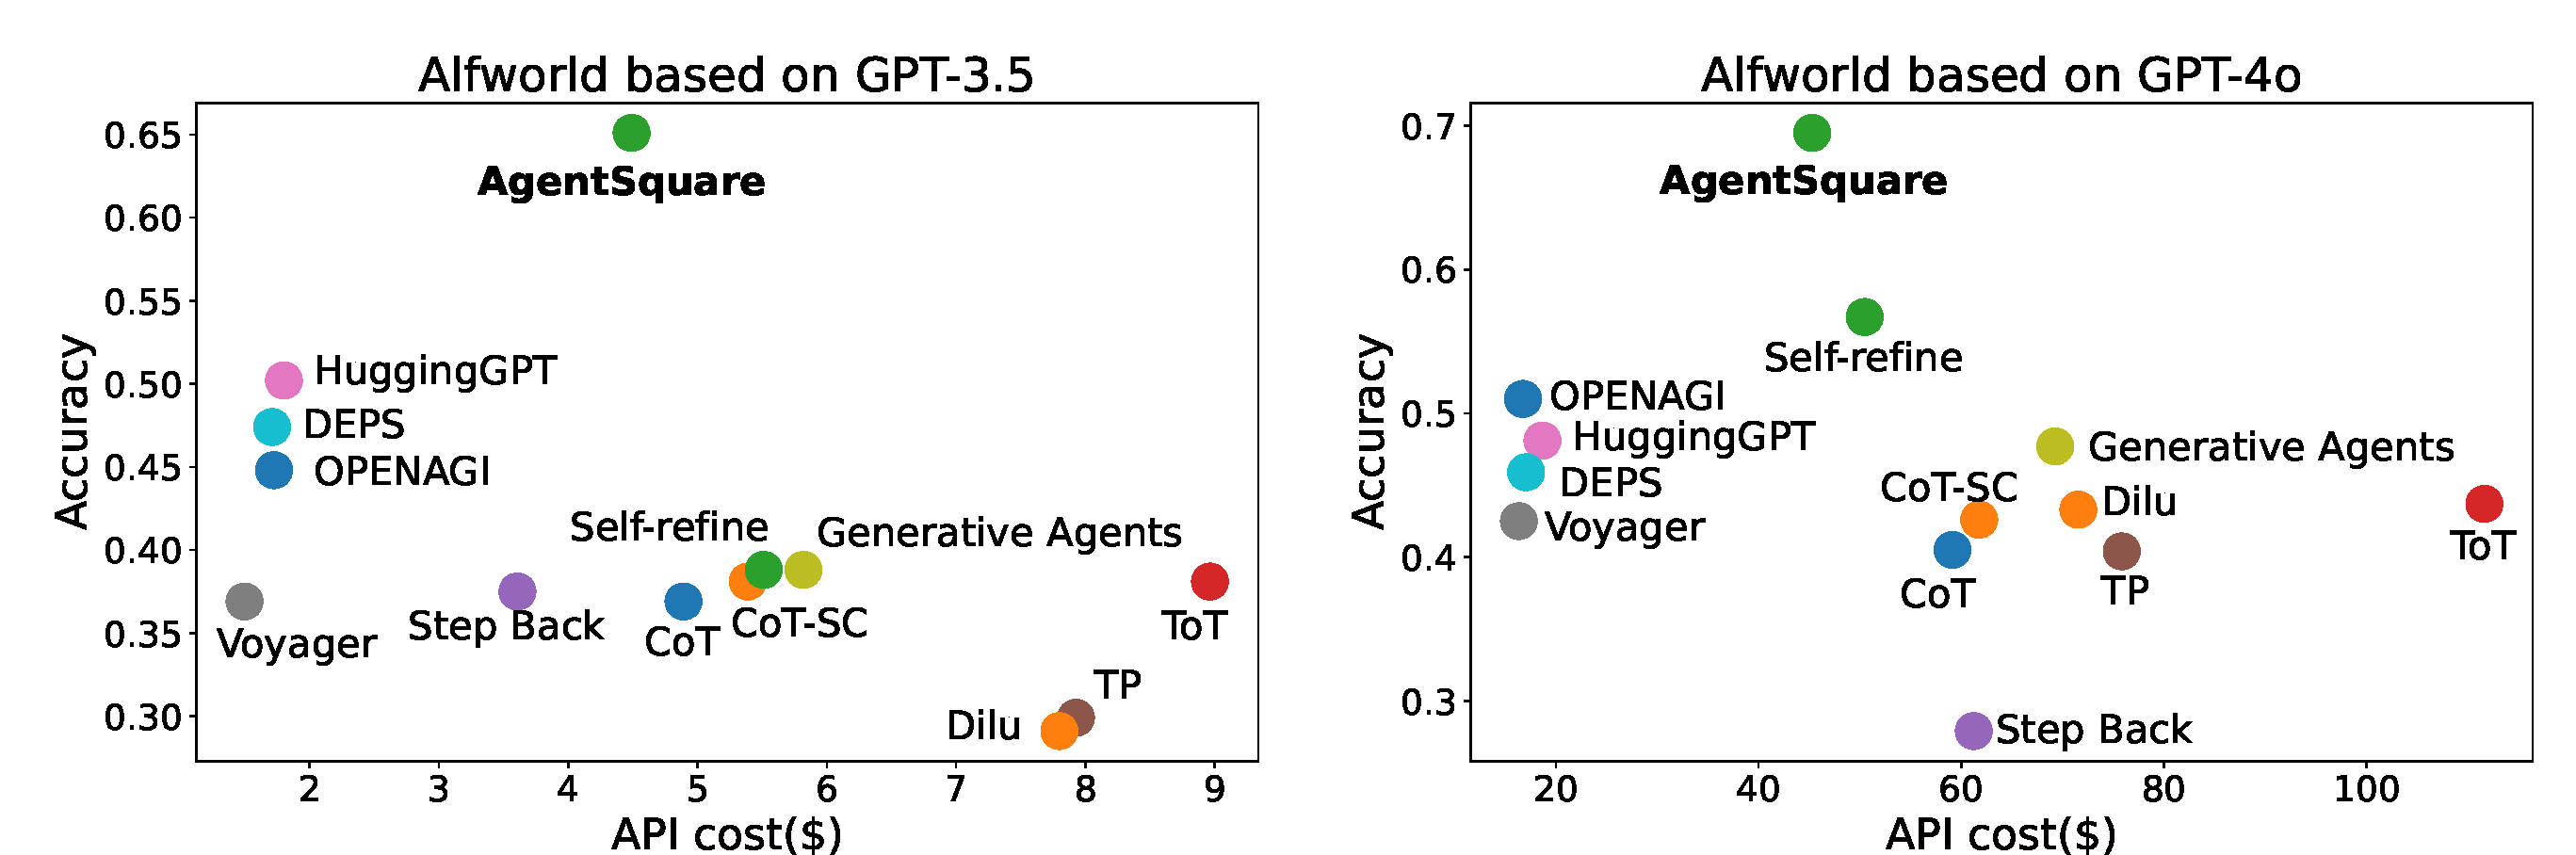
\includegraphics[width=\textwidth]{Figures/fig4_alfworld.pdf}
% % \includegraphics[width=12.5cm]{Figures/f4(sci).pdf}
% % \includegraphics[width=12.5cm]{Figures/f4(travel).pdf}
% %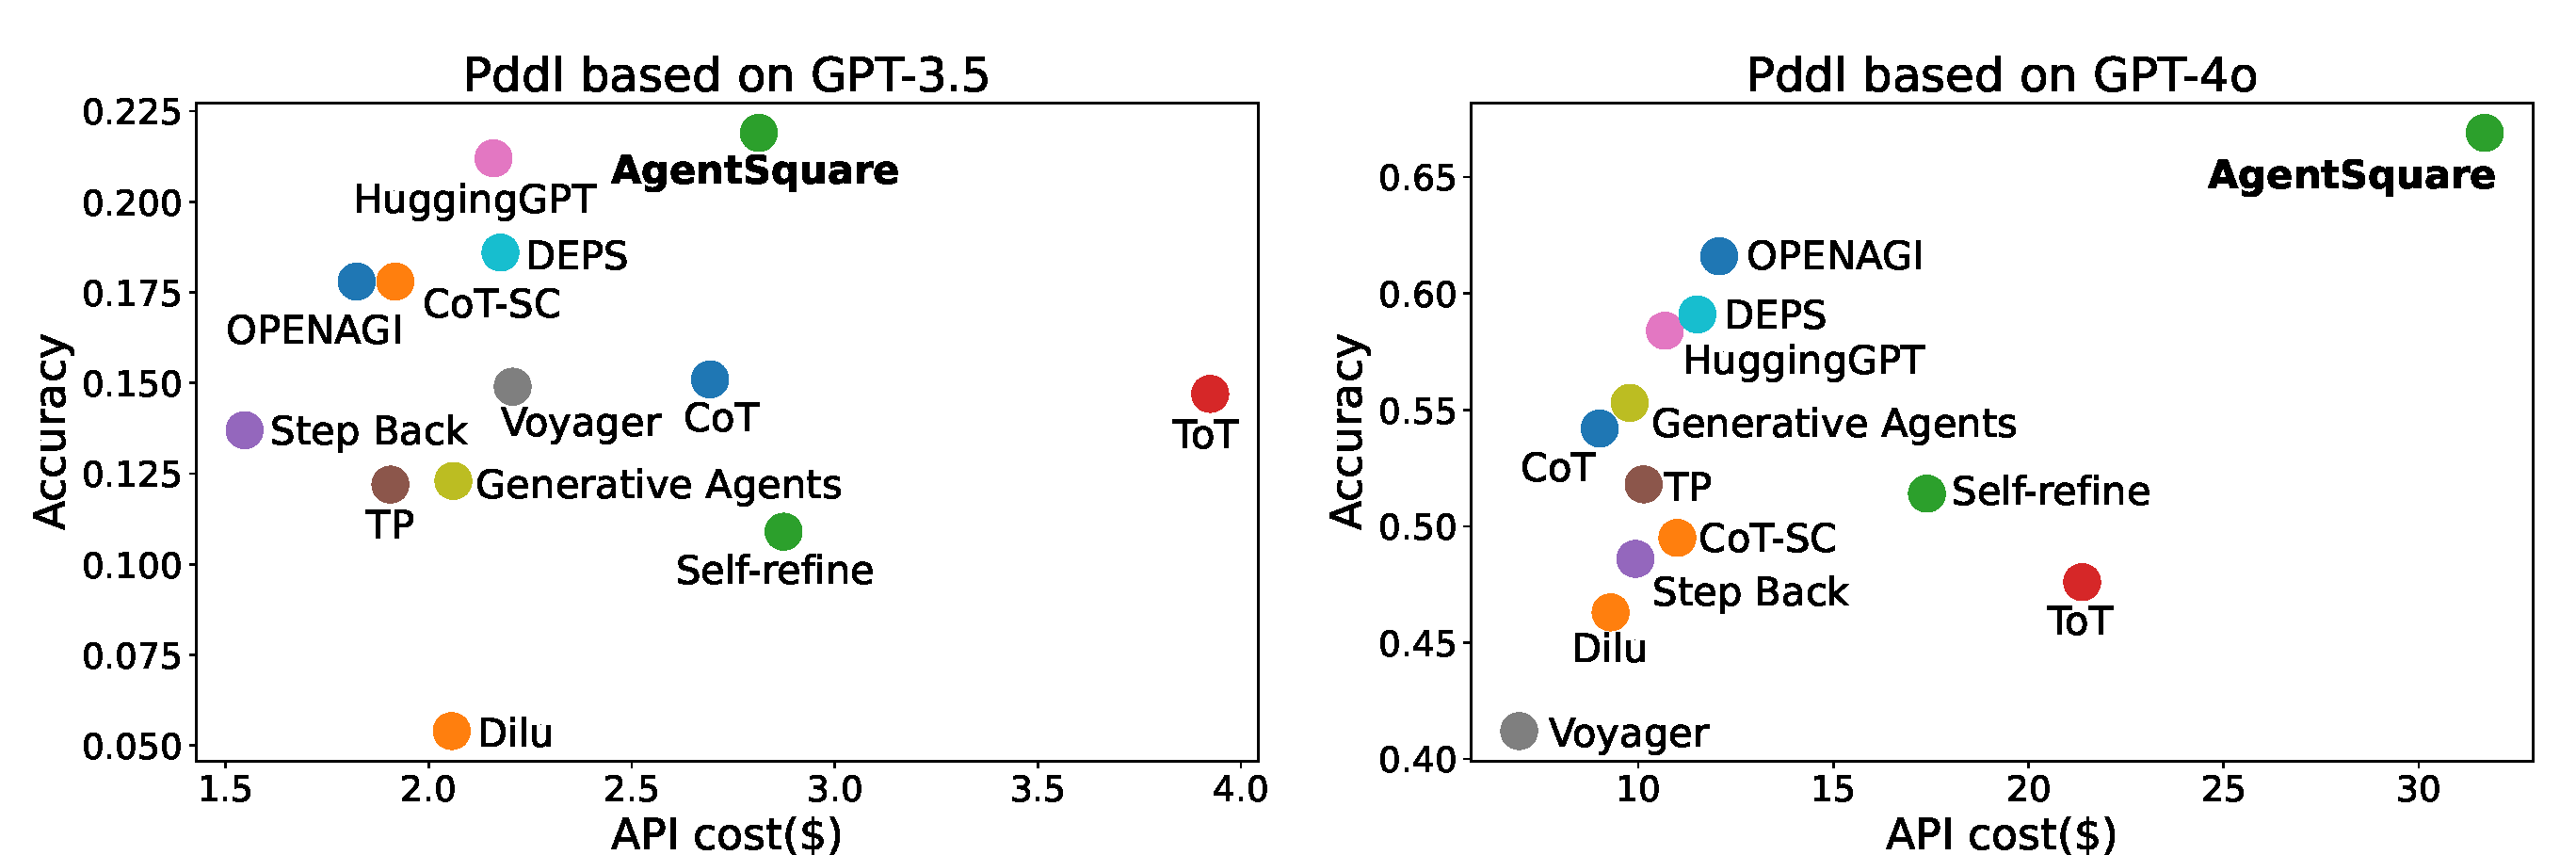
\includegraphics[width=12.5cm]{Figures/fig4_pddl.pdf}
% \caption{Performance versus API costs visualization on each task.}
% \label{fig4:performance-cost}
% \end{center}
% \end{figure}


\textbf{Search trajectory in AgentSquare.}
We present the search trajectory under 15 iterations using AgentSquare based on GPT-4o and other searching methods on ALFWorld and Webhop tasks in Figure~\ref{Fig7:trajectory}.
Results on other tasks are presented in Figure~\ref{app:trajectory1} and~\ref{app:trajectory2}.
AgentSquare demonstrates a steady convergence trajectory, where more advanced agents are continually emerging during search.
In contrast, module-level searching methods including random and Bayesian search lack a clear and insightful search direction.
Prompt-level search methods such as OPRO are constrained by a limited modification space, leading to minimal performance improvements.
As a result, they all encounter performance bottlenecks during the search process, resulting in sub-optimal agent architectures.
Besides, we find that simple module-level search methods such as random recombination greatly outperforms prompt-level search, indicating the importance of searching in the modular design space.  
\begin{figure}[!t]
\vspace{-6.5mm}
\begin{center}
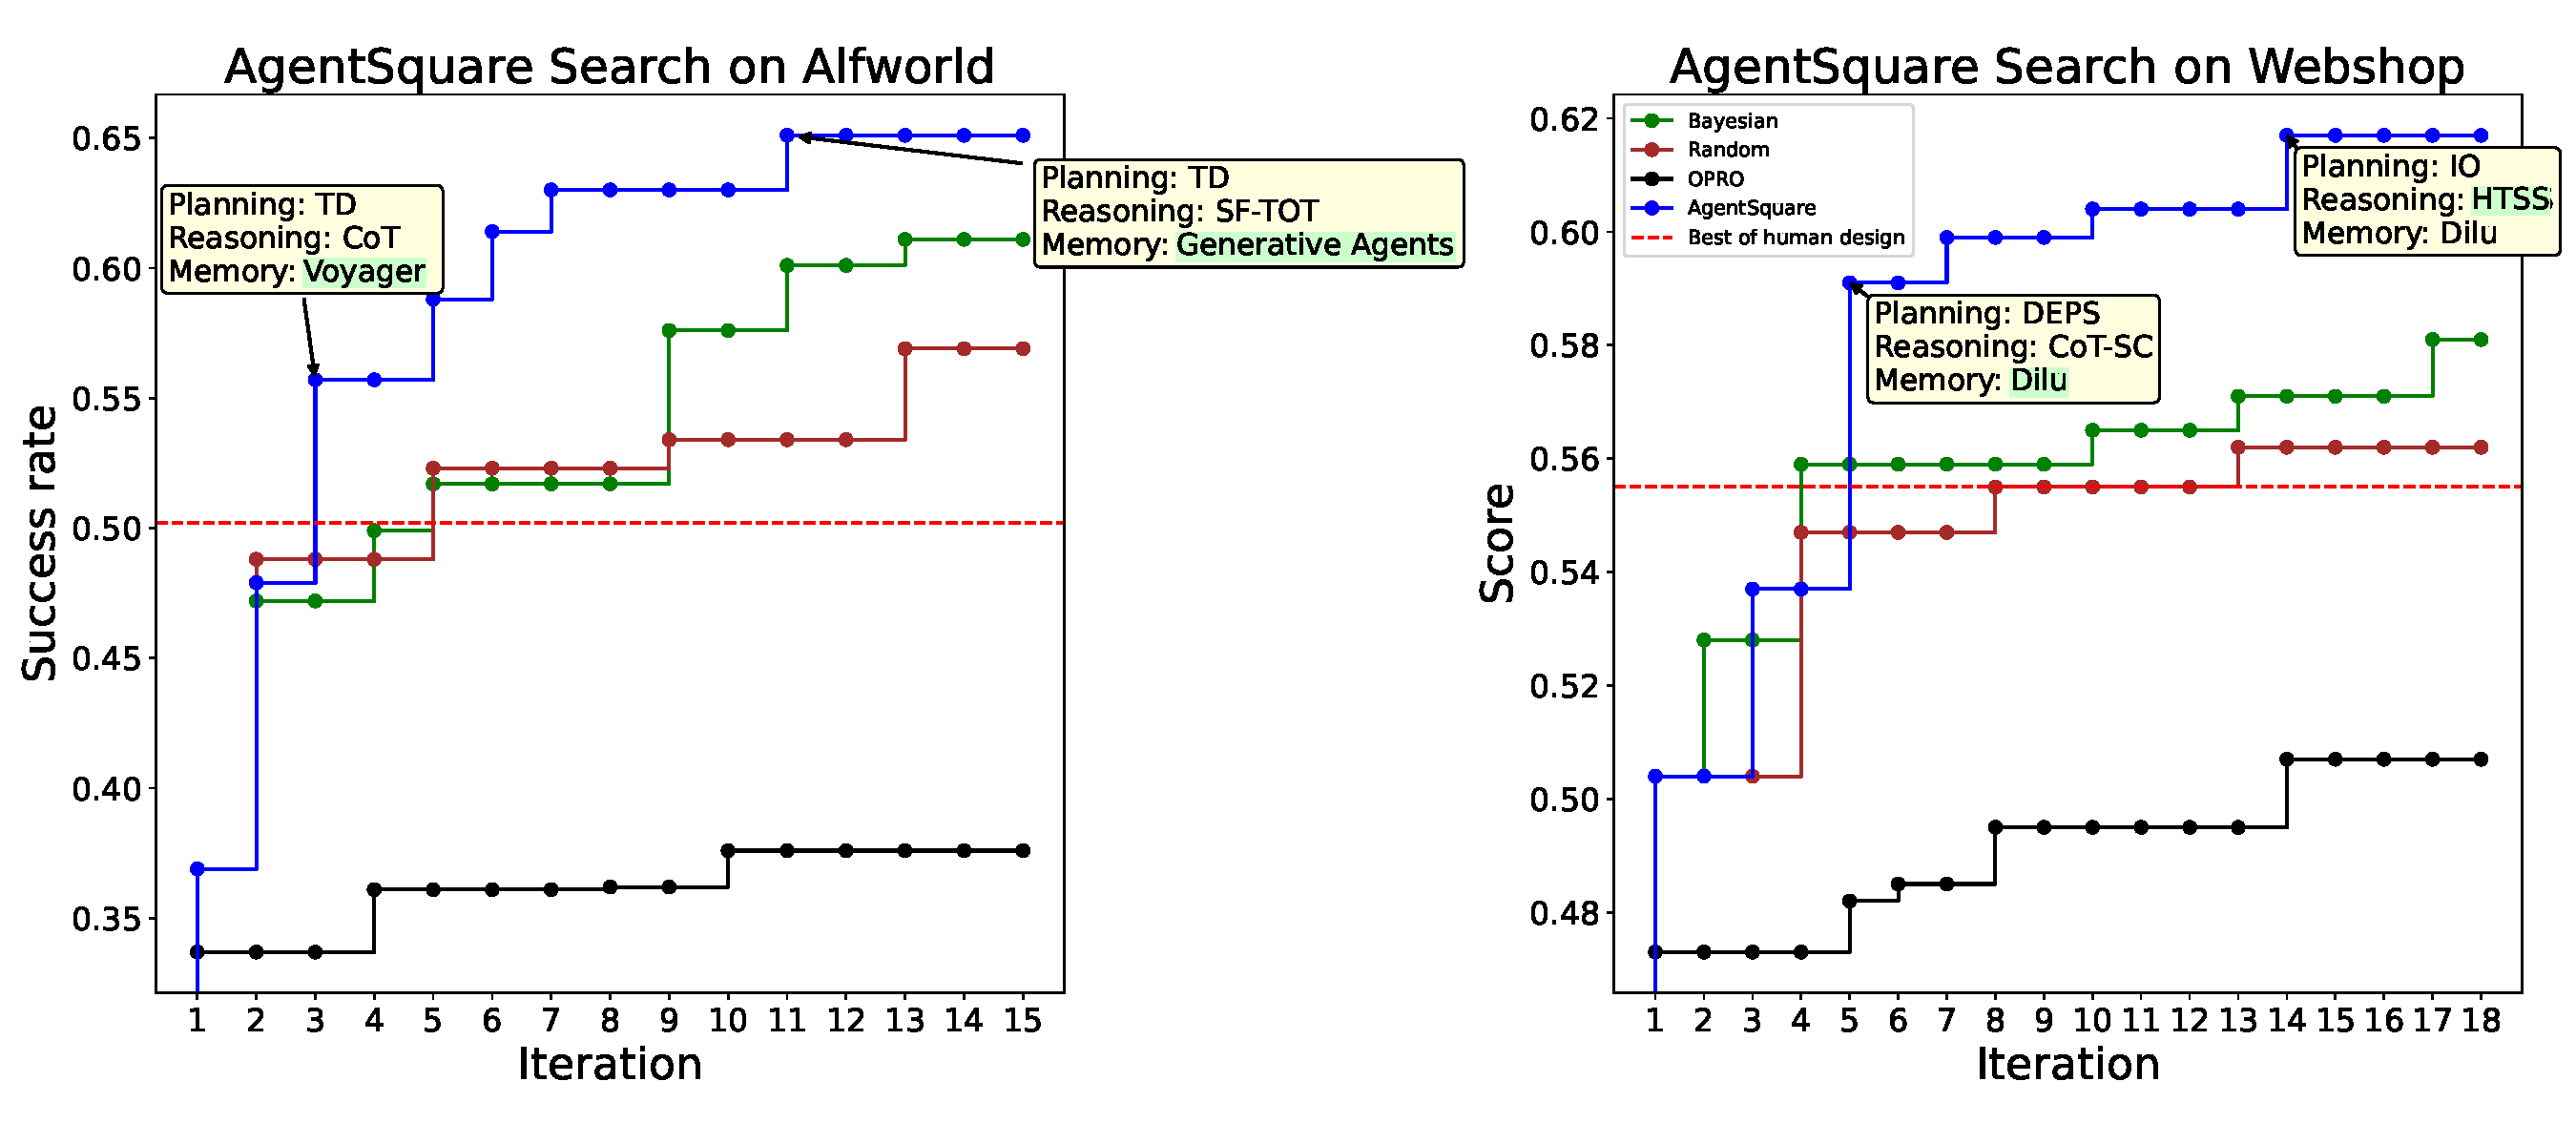
\includegraphics[width=0.8\textwidth]{Figures/fig5_alfworld_webshop.pdf}
\caption{AgentSquare search trajectory on Alfworld and Webshop.}
\vspace{-0.5em}
\label{Fig7:trajectory}
\end{center}
\end{figure}

\setlength{\tabcolsep}{1mm} 
\begin{table}[t!]
    \centering
    \begin{tabular}{cccccccc}
    \hline
    \textbf{Method} & \multicolumn{1}{c}{\textbf{Webshop}} & \multicolumn{1}{c}{\textbf{ALFWorld}} & \multicolumn{1}{c}{\textbf{SciWorld}} & \multicolumn{1}{c}{\textbf{M3Tool}} & \multicolumn{1}{c}{\textbf{TravelPlanner}}  
     & \multicolumn{1}{c}{\textbf{PDDL}}\\
    % \cmidrule(lr){2-5} \cmidrule(lr){6-9} \cmidrule(lr){10-12} \cmidrule(lr){13-15}
         % & Acc & Acc& Acc& Acc& Acc& Acc& Acc\\ 
    \hline
    AgentSquare (full) & \textbf{0.607} & \textbf{0.695} &\textbf{0.781}& \textbf{0.524} &\textbf{0.583}&\textbf{0.669}\\ 
    w/o module evolution& 0.564 & 0.649 &0.736& 0.502 &0.577 &0.614\\
    w/o module recombination& 0.560 & 0.616 &0.710& 0.481 &0.280 &0.669\\
    % w/o both-level search & 0.518 & 0.564 &0.704& 0.469 &0.563&0.558\\ 
    \hline
    \end{tabular}
    {\caption{Ablation study of AgentSquare on GPT-4o on six tasks across different domains.}
    \label{tab:ab2}}
\end{table}
\subsection{Ablation Study of AgentSquare} \label{technical}
\textbf{Effectiveness of module evolution and recombination.}
There are two key operations in the searching framework of AgentSquare: module evolution which creates new modules and module recombination which strategically recombines existing ones.
To verify the effectiveness of each design, we tested three variants: the full model, a version without module evolution, and a version without module recombination.
The results based on GPT-4o and GPT-3.5 are presented in Table~\ref{tab:ab2} and Table~\ref{tab:ab1}, respectively.
It can be seen that dropping each design results in a noticeable performance decline and the module recombination has a larger impact.
Module recombination significantly expands the search space, reducing the risk of falling into a local optima. 
Meanwhile, module evolution facilitates the discovery of more advanced modules tailored to specific tasks. 
These two operations collaborate well ensuring the effectiveness of the search process in AgentSquare.

\begin{figure}[!t]
\begin{center}
%\fbox{\rule[-.5cm]{0cm}{4cm} \rule[-.5cm]{4cm}{0cm}}
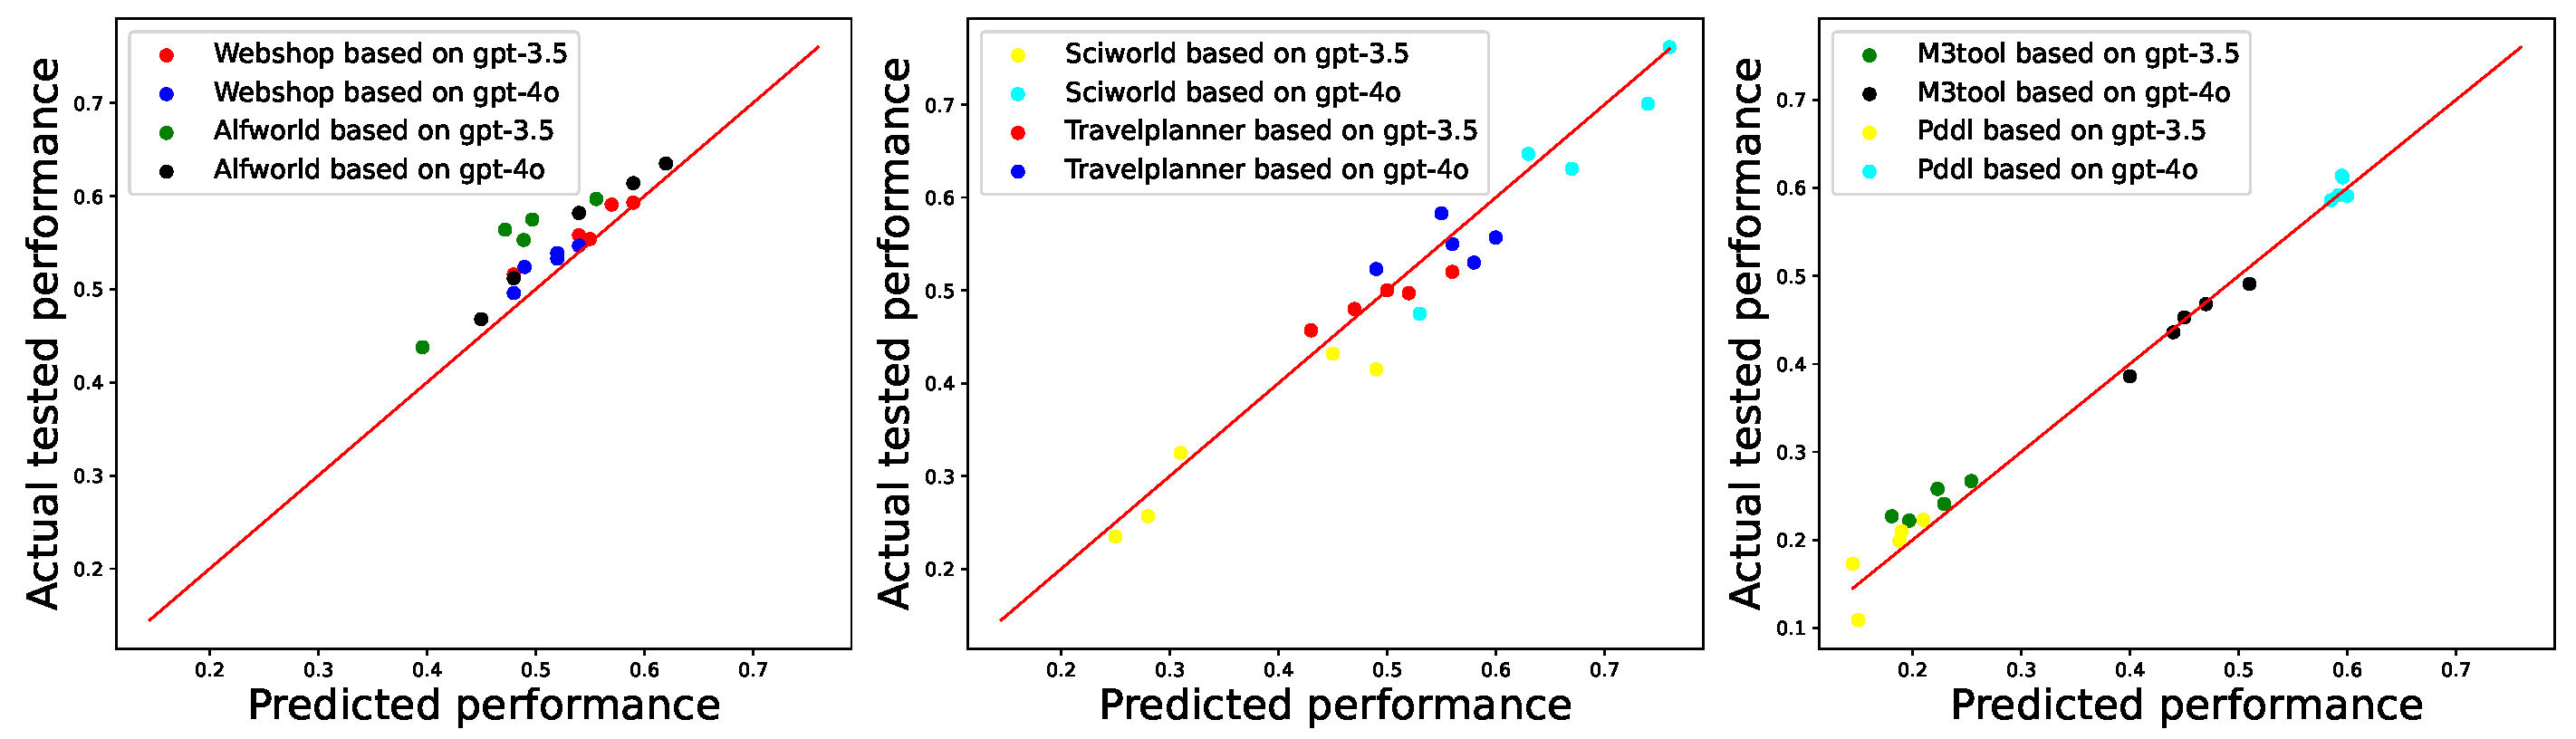
\includegraphics[width=0.85\textwidth]{Figures/fig6v0.pdf}
\caption{Validation of the effectiveness of the performance predictor (correlation between the actual and predicted performance) on each task.}
% \vspace{-3mm}
\label{pp}
\end{center}
\end{figure}

\textbf{Effectiveness of performance predictor.}
% To mitigate the high API costs associated with evaluating agents during the search process, we introduce an additional LLM as the performance predictor, inspired by existing practice utilizing LLM for neural architecture search~\citep{jawahar2023llm}.
In this part, we verify the effectiveness of this design empirically.
Figure~\ref{pp} illustrates the predicted performance of given agents versus their actual tested performance based on both GPT-3.5 and GPT-4o on all six tasks.
The tested agents were generated through random sampling by randomly combining existing modules. 
It can be found that the predicted performance closely aligns with the actual performance, demonstrating the effectiveness of the performance predictor.
For instance, the evaluation cost of the predictor is only about 0.025\% of the cost of a full evaluation based on GPT-4o in ALFWorld, demonstrating its remarkable cost-efficiency.
We provide more experiment results of predicting the performance of the dynamically searched agents in Figure~\ref{pp-search} of the Appendix.
\subsection{Discovered Best Agents from AgentSquare}
In this section, we provide some illustrations of the searched best agents, especially some discovered promising modules.
Table~\ref{tab:module} summarizes the searched best agent from AgentSquare and the best hand-crafted agents on all tasks.
We can observe that AgentSquare can adaptively identify promising agents with both previously existing and newly programmed modules tailored to the given task.
For instance, the discovered best agent for ALFWorld combines an existing well-designed memory module from \textit{Generative Agents} with newly created planning (named \textit{TD}) and reasoning modules (named \textit{SF-ToT}). 
By comparison, the best hand-crafted agent \textit{Self-refine} focuses only on reasoning module design while overlooking other functional modules, leading to suboptimal performance.
Moreover, we illustrate two new modules and the human interpretable design insights discovered on ALFWorld in Figure~\ref{main:New module}.
More illustrations are listed in the Figure~\ref{New module1} to Figure~\ref{New module6}.


% \setlength{\tabcolsep}{1.mm}         
% \begin{table}[t!]
%     \centering
%     \begin{tabular}{ccccc|c}
%     \hline
%     \textbf{Task} & \textbf{Planning} & \textbf{Reasoning} & \textbf{Tooluse} & \textbf{Memory} & \textbf{Best Hand-crafted Agents} \\ \hline
%     Webshop & IO & HTSS & / & Dilu & HuggingGPT \\ \hline
%     ALFWorld & TD & SF-ToT & / & Generative Agents& Self-refine \\ \hline
%     SciWorld & Voyager& CoT& / & Hier& Voyager\\ \hline
%     M3Tool & / & CoT-SC & ToolBF & / & Toolbench \\ \hline
%     TravelPlanner & DEPS & CoT & TH & / & DEPS \\ \hline
%     PDDL & IR & CASRC & / & Generative Agents& OPENAGI \\ \hline
%     \end{tabular}
%     {\caption{Comparison between the searched best agent from AgentSquare and the best human-designed agent on all tasks.}
%     \label{tab:module}}
% \end{table}

\begin{figure}[!t]
\begin{center}
%\fbox{\rule[-.5cm]{0cm}{4cm} \rule[-.5cm]{4cm}{0cm}}
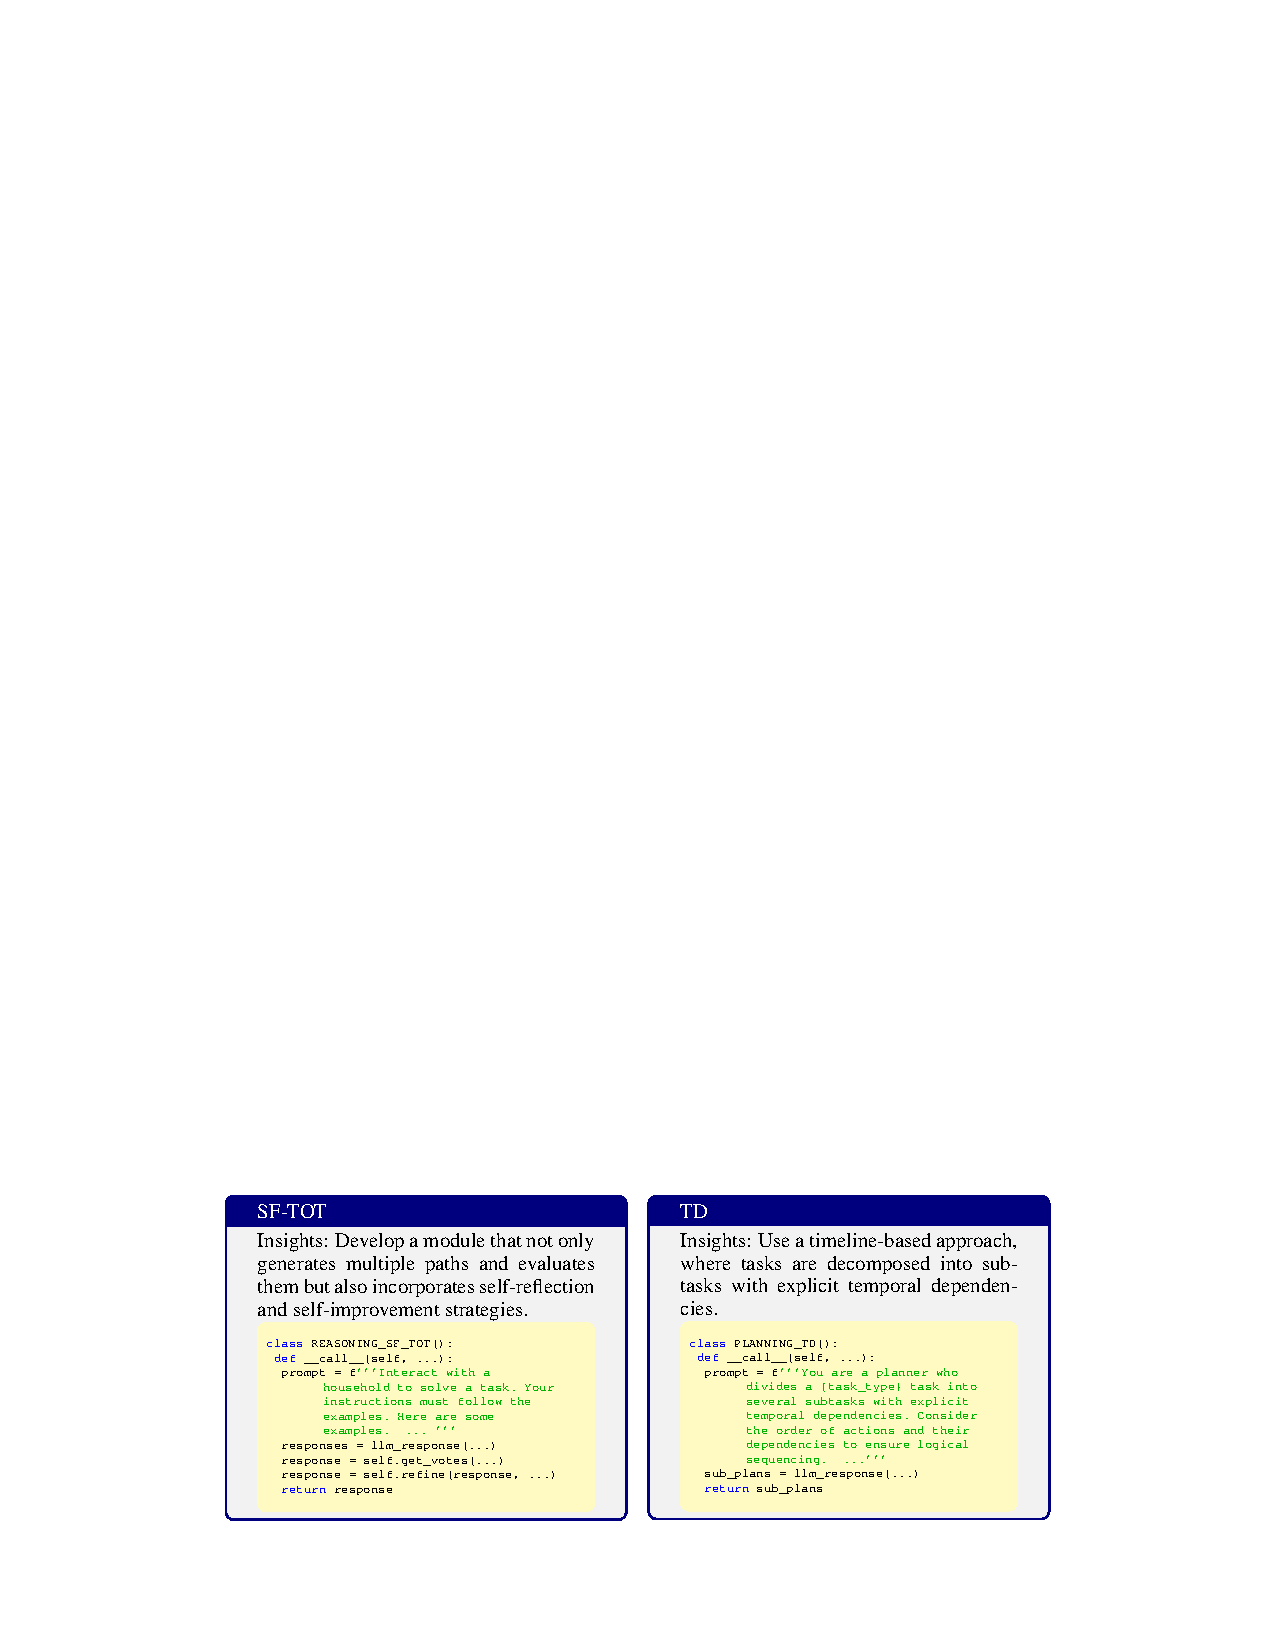
\includegraphics[width=0.8\textwidth]{Figures/new_module_alfworld.pdf}
\caption{New module discovered through AgentSquare search on ALFWorld.}
\label{main:New module}
\end{center}
\end{figure}



% \setlength{\tabcolsep}{1.5mm} 
% \begin{table}[t!]
%     \centering
%     \begin{tabular}{cccccccc}
%     \hline
%     \textbf{Method} & \multicolumn{1}{c}{\textbf{Webshop}} & \multicolumn{1}{c}{\textbf{ALFWorld}} & \multicolumn{1}{c}{\textbf{SciWorld}} & \multicolumn{1}{c}{\textbf{M3Tool}} & \multicolumn{1}{c}{\textbf{TravelPlanner}} & 
%      \multicolumn{1}{c}{\textbf{PDDL}}\\
%     % \cmidrule(lr){2-5} \cmidrule(lr){6-9} \cmidrule(lr){10-12} \cmidrule(lr){13-15}
%          % & Acc & Acc& Acc& Acc& Acc& Acc& Acc\\ 
%     \hline
%         % IO & 0.473 & 0.306 & 0.105& 0.158  &0.043 & 0.166\\ 
%         CoT & 0.504 & 0.369 & 0.142 & 0.172 &0.080& 0.151\\ 
%         CoT-SC & 0.527 & 0.381 & 0.105& 0.181  & 0.167& 0.178\\ 
%         Self-refine & 0.439 & 0.388 & 0.222& 0.098  & 0.000& 0.109\\ 
%         ToT & 0.510 & 0.381 & 0.143 & 0.189  & 0.163& 0.147\\ 
%         Step Back & 0.478 & 0.375 &0.027& 0.128  & 0.120& 0.137\\ 
%         Thought Propagation & 0.429 & 0.299 &0.168& 0.139  & 0.063 & 0.122\\ 
%         % toolformer & / & / & /& 0.194  & 0.000& / \\ 
%         % toolbench & / & / & /& 0.204  & 0.053& / \\ 
%         % anytool & / & / & /& 0.139  & 0.077&  / \\ 
%         HuggingGPT & 0.518 & 0.502 & 0.27& 0.012  &0.470 & 0.212 \\ 
%         Voyager & 0.427 & 0.369 & 0.301& 0.008&0.480 &0.149\\ 
%         Generative Agents & 0.539 & 0.388 & 0.153& 0.144  & 0.060& 0.123 \\ 
%         DEPS & 0.555 & 0.474 & 0.308 & 0.017  & 0.500& 0.186\\ 
%         OPENAGI & 0.507 & 0.448 & 0.257 & 0.008  & 0.430& 0.178\\ 
%         Dilu & 0.418 & 0.291 &0 & 0.131 &0.137 &0.054\\ 
%         Random Recombination & & & & & & \\
%         Bayesian Recombination & & & & & & \\
%         PromptBreeder & & & & & &  \\
%         OPRO & & & & & & \\
%    \textbf{AgentSquare} & 0.617 & 0.651 &0.432& 0.285&0.520&0.219 \\ \hline
%     \end{tabular}
%     {\caption{Performance comparison of searched agents from AgentSquare and existing human-designed agents based on GPT-3.5 on six tasks across different domains (add task domains).}
%     \label{tab:main1}}
% \end{table}




% \setlength{\tabcolsep}{1.5mm} 
% \begin{table}[t!]
%     \centering
%     \begin{tabular}{cccccccc}
%     \hline
%     \textbf{Method} & \multicolumn{1}{c}{\textbf{Webshop}} & \multicolumn{1}{c}{\textbf{ALFWorld}} & \multicolumn{1}{c}{\textbf{SciWorld}} & \multicolumn{1}{c}{\textbf{M3Tool}} & \multicolumn{1}{c}{\textbf{TravelPlanner}} & 
%      \multicolumn{1}{c}{\textbf{PDDL}}\\
%     % \cmidrule(lr){2-5} \cmidrule(lr){6-9} \cmidrule(lr){10-12} \cmidrule(lr){13-15}
%          % & Acc & Acc& Acc& Acc& Acc& Acc& Acc\\ 
%     \hline
%         % IO & 0.411 & 0.367 & 0.759& 0.439 & 0.407& 0.559\\ 
%         CoT & 0.485 & 0.405 & 0.697& 0.448  & 0.487 & 0.542\\ 
%         Cot-SC & 0.512 & 0.426 & 0.656 & 0.461  & 0.413& 0.495\\ 
%         Self-refine & 0.461 & 0.567 & 0.654 & 0.442  & 0.000& 0.514\\ 
%         ToT & 0.501 & 0.437 & 0.741& 0.453  &0.380 & 0.476\\ 
%         Step Back & 0.468 & 0.279 & 0.220 & 0.434  & 0.000& 0.486\\ 
%         Thought Propagation & 0.398 & 0.404 & 0.576 & 0.387  & 0.430& 0.518\\ 
%         % toolformer & / & / & / & 0.449  & 0.510& / \\ 
%         % toolbench & / & / & /& 0.469  & 0.000 &  / \\ 
%         % anytool & / & / & / & 0.375  & 0.523& / \\ 
%         HuggingGPT & 0.519 & 0.481 & 0.680& 0.354  & 0.510& 0.584\\ 
%         Voyager & 0.366 & 0.425 & 0.776& 0.247 &0.523 &0.412\\ 
%         Generative Agents & 0.499 & 0.477 & 0.663& 0.402  & 0.480& 0.553\\ 
%         DEPS & 0.481 & 0.459 & 0.740 & 0.278 & 0.540& 0.591\\ 
%         OPENAGI & 0.506 & 0.510 & 0.718& 0.322  & 0.533 & 0.616\\ 
%         Dilu & 0.451 & 0.433 & 0.682 & 0.475 &0.360 &0.463\\ 
%         Random Recombination & & & & & & \\
%         Bayesian Recombination & & & & & & \\
%         PromptBreeder & & & & & &  \\
%         OPRO & & & & & & \\
%     \textbf{AgentSquare} & 0.607 & 0.695 & 0.781& 0.524 &0.583 &0.669\\  \hline
%     \end{tabular}
%     {\caption{Performance comparison of searched agents from AgentSquare and existing human-designed agents based on GPT-4 on six tasks across different domains.}
%     \label{tab:main2}}
% \end{table}






% \begin{figure}[!t]
% \begin{center}
% \fbox{\rule[-.5cm]{0cm}{4cm} \rule[-.5cm]{4cm}{0cm}}
% \caption{Analysis for LLM agent design choices in 4 dimensions over different tasks.}
% \label{module-level}
% \end{center}
% \end{figure}

% \setlength{\tabcolsep}{3mm}         
% \begin{table}[t!]
%     \centering
%     \begin{tabular}{cccccc}
%     \hline
%     \textbf{Task} & \textbf{Agent Type} &\textbf{Planning} & \textbf{Reasoning} & \textbf{Tooluse} & \textbf{Memory} \\ \hline
%     \multirow{2}{*}{Webshop} & Hand-crafted Agents & hugginggpt & IO & / & / \\
%                              & AgentSquare search & IO & cot-sc & / & dilu \\ \hline
%     \multirow{2}{*}{ALFWorld} & Hand-crafted Agents & / & self-refine & / & / \\
%                              & AgentSquare search & RP & SF_TOT & / & generative \\ \hline
%     \multirow{2}{*}{SciWorld} & Hand-crafted Agents &DEPS &IO &/&/ \\
%                              & AgentSquare search &Adaptive &IO &/&/ \\ \hline
%     \multirow{2}{*}{M3Tool} & Hand-crafted Agents & / & / & toolbench & / \\
%                              & AgentSquare search & / & cot-sc & toolbench & / \\ \hline
%     \multirow{2}{*}{TravelPlanner} & Hand-crafted Agents &DEPS &IO &IO&/ \\
%                                    & AgentSquare search &DEPS &COT &TH&/ \\ \hline
%     \multirow{2}{*}{PDDL} & Hand-crafted Agents &OPENAGI & IO &/ & / \\
%                           & AgentSquare search &self-refine-COT & Iterative-refine&/&generative \\ \hline
%     \end{tabular}
%     {\caption{Comparison between the searched best agent from AgentSquare and the best human-designed agent on all tasks (show prompts of searched modules, only show the best human-design agent's name).}
%     \label{tab:main2}}
% \end{table}

% \setlength{\tabcolsep}{1.mm}         
% \begin{table}[t!]
%     \centering
%     \begin{tabular}{ccccc|c}
%     \hline
%     \textbf{Task} & \textbf{Planning} & \textbf{Reasoning} & \textbf{Tooluse} & \textbf{Memory} & \textbf{Best Hand-crafted Agents} \\ \hline
%     Webshop & IO & HTSS & / & Dilu & HuggingGPT \\ \hline
%     ALFWorld & RP & SF-TOT & / & Generative Agents& Self-refine \\ \hline
%     SciWorld & Adaptive & IO & / & / & DEPS \\ \hline
%     M3Tool & / & CoT-SC & ToolBF & / & Toolbench \\ \hline
%     TravelPlanner & DEPS & COT & TH & / & DEPS \\ \hline
%     PDDL & Self-refine-COT & Iterative-refine & / & Generative Agents& OPENAGI \\ \hline
%     \end{tabular}
%     {\caption{Comparison between the searched best agent from AgentSquare and the best human-designed agent on all tasks (show prompts of searched modules).}
%     \label{tab:main2}}
% \end{table}


% \setlength{\tabcolsep}{1mm} 
% \begin{table}[t!]
%     \centering
%     \begin{tabular}{cccccccc}
%     \hline
%     \textbf{Method} & \multicolumn{1}{c}{\textbf{Webshop}} & \multicolumn{1}{c}{\textbf{ALFWorld}} & \multicolumn{1}{c}{\textbf{SciWorld}} & \multicolumn{1}{c}{\textbf{M3Tool}} & \multicolumn{1}{c}{\textbf{TravelPlanner}}  
%      & \multicolumn{1}{c}{\textbf{PDDL}}\\
%     % \cmidrule(lr){2-5} \cmidrule(lr){6-9} \cmidrule(lr){10-12} \cmidrule(lr){13-15}
%          % & Acc & Acc& Acc& Acc& Acc& Acc& Acc\\ 
%     \hline
%     AgentSquare (full) & \textbf{0.617} & \textbf{0.651} &\textbf{0.432}& \textbf{0.285} &\textbf{0.520}&\textbf{0.219}\\ 
%     w/o module evolution& 0.595 & 0.623 &0.288& 0.236 &0.483&0.202 \\
%     w/o module recombination& 0.578 & 0.546 &0.310& 0.258 & 0.267&0.173\\
%     % w/o both-level search& 0.555 & 0.512 &0.367& 0.204 &0.473&0.159 \\ 
%     \hline
%     \end{tabular}
%     {\caption{Ablation study of AgentSquare on GPT-3.5 on six tasks across different domains.}
%     \label{tab:ab1}}
% \end{table}



\section{Related Work}
\subsection{LLM-based Autonomous Agents}
LLM-based autonomous agents are an advanced AI system using a core LLM to manage external functional modules and interact with the world~\citep{ding2024understanding}.  
%In the early stage, LLM-based agents possess very simple architectures, which just directly query LLMs to conduct decision-making and take action~\citep{huang2022language,ahn2022can}. 
Recent studies have equipped LLM agents with several LLM-centric functional modules including planning~\citep{hao2023reasoning,zeng2024perceive,shao2025division}, reasoning~\citep{wei2022chain,yao2024tree,shang2024defint,xu2025towards}, using tools~\citep{shen2024hugginggpt,schick2024toolformer}, and monitoring memory~\citep{wang2024voyager,park2023generative}, greatly enhancing the capabilities of LLM agents. 
Along with the improvement of the single agent, there's another line of work trying to build more advanced multi-agent systems by strategically organizing individual agents for both simulation~\citep{li2023metaagents,chen2023agentverse} and targeted task solving~\citep{qian2024chatdev,chen2024large,li2024limp}.
The emergence of more and more sophisticated agent produces remarkable performance improvement, however, their architectures and codebases differ greatly with each other.
The lack of a unified design space and consistent terminologies across individual works makes it hard to compare different agents, understand their evolution routes, and guide new agent design directions.



\subsection{Automatic Design of LLM-based Agents}
LLM-based agent system, as the most advanced AI system, has not yet formed a unified design space and an automatic design approach.
%Existing efforts on automatic building of LLM agents focus on three aspects: engineering-oriented open resources, conceptual framework of LLM agent design, and automatic design of partial components of LLM agents.
Engineering-oriented open resources like LangChain\footnote{https://github.com/langchain-ai/langchain} and BabyAGI\footnote{https://github.com/yoheinakajima/babyagi} have provided convenient ways to build an LLM-centric agentic system, however, they still need human participation to organize different modules and can't support the optimization of the designed agent.
Besides, there have been some conceptual frameworks trying to provide a unified design principle of LLM agents, such as CoALA~\citep{sumers2023cognitive}. 
%It points out four basic modules of language agents from the perspective of cognitive science, including long-term memory, external grounding, internal actions and decision-making.
However, it's still a vision of how LLM agents should be in the future, without providing a practical design framework.
More importantly, there are several recent works that explore the problem of automating (at least part of) the design of LLM agent systems defined on different search spaces. OPRO~\citep{yang2024large} and Promptbreeder~\citep{fernando2024promptbreeder} can be considered as using LLMs to optimize LLM agent defined on prompt space. More relevantly, ADAS~\citep{hu2024automated} proposes to search the entire agentic system defined on code space, enabling the search for LLM agents with more flexible prompts, tool uses, control flows and more.


% Nevertheless, these works over-simplify the structure of agentic systems to pure prompts or codes, unable to provide a clear design space of LLM agents.
% Besides, another common shortcoming of existing works is that all of them are proposed without much consideration of existing designed agent architectures, thus hard to be representative and universal.
% Differently, our proposed modularized LLM agent design space can well cover existing efforts of LLM agent design, and provide a practical approach for automatic agent architecture optimization.


\section{Conclusion}
In this work, we introduce a novel modular design space for LLM agents, allowing researchers to build upon successful prior designs and collectively accumulate new insights. 
Based on this, we propose a novel research problem, Modularized LLM Agent Search (MoLAS), which aims to automatically optimize LLM agent designs by leveraging the knowledge gained from previously published or evaluated modules.
To address the challenge of vast search spaces, we present AgentSquare, an automatic search framework to optimize LLM agents through module evolution and recombination.
We further introduce a performance predictor as an in-context surrogate model for evaluating novel LLM agents to accelerate the search process.
% AgentSquare consistently discovers novel agents that surpass all existing hand-crafted ones. 
Overall, our work offers a transition from studying individual LLM agent designs to studying LLM agents within a modular design space, further consolidating the collective efforts of the research community.
% AgentSquare consistently discovers novel agents that outperform all existing hand-crafted agents. 
% Additionally, it provides interpretable design insights, further enhancing the understanding of these newly discovered agents.
% AgentSquare consistently discovers novel agents that outperform all existing hand-crafted agents. 
% Additionally, it provides interpretable design insights, further enhancing the understanding of these newly discovered agents.
\clearpage

% \subsubsection*{Acknowledgments}


\bibliography{ref}
\bibliographystyle{iclr2025_conference}

\appendix
\clearpage
\section{Appendix}
\renewcommand{\thefigure}{A.\arabic{figure}}
\renewcommand{\thetable}{A.\arabic{table}}
\subsection{Experimental Setup} \label{app:setup}
\textbf{Task setup.}
We evaluate AgentSquare and compared methods on six representative tasks covering four key domains which are widely adopted by existing LLM agent benchmarks~\citep{ma2024agentboard,xi2024agentgym}: 
\begin{itemize}[leftmargin=*]
    \item \textbf{Embodied:} ALFWorld~\citep{shridhar2021alfworld} with text-based household tasks where agents navigate and interact with objects using text commands, ScienceWorld~\citep{wang2022scienceworld} with interactive science tasks requiring agents to navigate rooms and perform experiments, testing scientific commonsense; 
    \item \textbf{Game:} PDDL~\citep{ma2024agentboard} including many strategic games where agents use PDDL expressions to complete tasks; 
    \item \textbf{Web:} WebShop~\citep{yao2022webshop} focusing on online shopping tasks where agents browse and purchase products based on user instructions; 
    \item \textbf{Tool:} TravelPlanner~\citep{xie2024travelplanner} with many travel planning tasks where agents use tools and data to create detailed plans, (6)M3ToolEval~\citep{wang2024executable} including complex tasks requiring multi-turn interactions with multiple tools.
\end{itemize}
The specific performance evaluation metric varies in different tasks, following the evaluation settings in their original work. Specifically, the evaluation metric is ``success rate'' for ALFWorld and M3ToolEval, ``task score (defined as the average reward obtained across episodes)'' for Webshop, ``progress rate'' for SciWorld and PDDL, and ``micro pass rate'' for TravelPlanner.

\textbf{Baselines.}
We compare AgentSquare with four types of baselines:
\begin{itemize}[leftmargin=*]
    \item \textbf{Hand-crafted agents.} We compare with 12 hand-crafted agents including CoT~\citep{wei2022chain}, CoT-SC~\citep{wang2023selfconsistency}, Self-refine~\citep{madaan2024self}, ToT~\citep{yao2024tree}, Step back~\citep{zheng2024take}, Thought propagation~\citep{yu2024thought}, HuggingGPT~\citep{shen2024hugginggpt}, Voyager~\citep{wang2024voyager}, Generative Agents~\citep{park2023generative}, DEPS~\citep{wang2024describe}, OPENAGI~\citep{ge2024openagi}and Dilu~\citep{wen2024dilu}. 
    \item \textbf{Module search methods.} We compare with two module-level agent optimization methods including the random combination of existing modules and Bayesian~\citep{zhou2019bayesnas} module combination optimization inspired by Bayesian optimization in NAS~\citep{white2021bananas}.
    \item \textbf{Prompt search methods.} 
    We select OPRO~\citep{yang2024large} as a representative prompt-level optimization approach, which leverages LLMs as optimizers by generating and refining instructions through iterative prompts.
    \item \textbf{Agent search methods.} We select ADAS~\citep{hu2024automated} which optimizes the entire agentic system in code space as the agent search baseline. We use the official code of ADAS and make slight modifications to adapt it to our tasks. 
    % The modifications are mainly on three aspects: (1) adjusting the task descriptions, instructions and examples in the meta prompt; (2) replacing the fitness value of each agent with its performance on our tasks; and (3) changing the evaluation procedure to align with our tasks.
\end{itemize}

\textbf{AgentSquare setup.}
We implement AgentSquare and conduct experiments using both GPT-3.5-turbo-0125 and GPT-4o~\citep{achiam2023gpt}. To ensure a fair comparison, we use the same number of few-shot examples across all methods. The initial agent is set as a random module combination, and the search process terminates after 5 consecutive iterations without performance improvement.

\begin{algorithm}[t!] 
% \SetAlgoNoLine 
\caption{Algorithm of AgentSquare} 
\label{alg}
% \LinesNumbered 
\KwIn{
Initial agent $A_0$, targeted task descriptions $d$, maximum evolution episode $K$,  population size $N$ per evolution phase, standardized module pools $\{\mathbb{P}, \mathbb{R}, \mathbb{T}, \mathbb{M}\}$, experience pool $\mathbb{E}$ 
}
\KwOut{The evolved agent $A^*$}
$t \leftarrow 1$ \tcp{Current search episode}
$A_e^0 \leftarrow A_0$  \tcp{Initialization of the module evolution phase} 
\While{$t \leq K$}{
$\{A_e^1,A_e^2,...,A_e^N\} \leftarrow \pi_{\xi} (A_e^0, d, N, \mathbb{P}, \mathbb{R}, \mathbb{T}, \mathbb{M}, \mathbb{E})$ 
\tcp{Module evolution}
$A_r^0 \leftarrow \argmax\{{Eval}_d(A_e^0), {Eval}_d(A_e^1),...,{Eval}_d(A_e^N)\}$  \tcp{Select the best-performing generated agent} 
$\{A_r^1,A_r^2,...,A_r^N\} \leftarrow \pi_{\theta} (A_r^0, d, N, \mathbb{P}, \mathbb{R}, \mathbb{T}, \mathbb{M}, \mathbb{E})$ \tcp{Module recombination} 
$A_e^0 \leftarrow \argmax\{{Eval}_d(A_r^0), {Eval}_d(A_r^1),...,{Eval}_d(A_r^N)\}$ \tcp{Select the best-performing generated agent} 
$ t \leftarrow t+1$ 
}

$A^* \leftarrow A_e^0$ 

\Return $A^*$
\end{algorithm}

\setlength{\tabcolsep}{0.5mm} 
\begin{table}[t!]
    \centering
    \begin{tabular}{cccccccc}
    \hline
    & & \textbf{Web} & \multicolumn{2}{c}{\textbf{Embodied}} & \multicolumn{2}{c}{\textbf{Tool}} & \textbf{Game} \\ 
    \hline
    \textbf{Method Type} & \textbf{Method} & \multicolumn{1}{c}{\textbf{Webshop}} & \multicolumn{1}{c}{\textbf{ALFWorld}} & \multicolumn{1}{c}{\textbf{SciWorld}} & \multicolumn{1}{c}{\textbf{M3Tool}} & \multicolumn{1}{c}{\textbf{Travel}} & \multicolumn{1}{c}{\textbf{PDDL}}\\
    \hline
    \multirow{13}{*}{Hand-crafted Agents} 
        & CoT & 0.504 & 0.369 & 0.142 & 0.172 &0.080& 0.151\\ 
        & CoT-SC & 0.527 & 0.381 & 0.105& 0.181  & 0.167& 0.178\\ 
        & Self-refine & 0.439 & 0.388 & 0.222& 0.098  & 0.000& 0.109\\ 
        & ToT & 0.510 & 0.381 & 0.143 & 0.189  & 0.163& 0.147\\ 
        & Step Back & 0.478 & 0.375 &0.027& 0.128  & 0.120& 0.137\\ 
        & TP & 0.429 & 0.299 &0.168& 0.139  & 0.063 & 0.122\\ 
        & HuggingGPT & 0.518 & 0.502 & 0.270& 0.012  &0.470 & 0.212 \\ 
        & Voyager & 0.427 & 0.369 & 0.301& 0.008&0.480 &0.149\\ 
        & Generative Agents & 0.539 & 0.388 & 0.153& 0.144  & 0.060& 0.123 \\ 
        & DEPS & 0.555 & 0.474 & 0.308 & 0.017  & 0.500& 0.186\\ 
        & OPENAGI & 0.507 & 0.448 & 0.257 & 0.008  & 0.430& 0.178\\ 
        & Dilu & 0.418 & 0.291 &0.000& 0.131 &0.137 &0.054\\ 
    \hline
    \multirow{2}{*}{Module Search} 
        & Random  & 0.562 & 0.569 & 0.367& 0.235 & 0.473&0.216 \\
        & Bayesian & 0.581 & 0.611 & 0.269& 0.217 & 0.497&0.210 \\
    \hline
    \multirow{1}{*}{Prompt Search} 
        % & PromptBreeder & & & & & &  \\
        & OPRO & 0.507 & 0.376 & 0.032& 0.193 & 0.513& 0.179\\
    \hline
    \multirow{1}{*}{Agent Search} 
        & ADAS & 0.519 & 0.274 & 0.217 & 0.193 & 0.410 & 0.186 \\
    \hline
    \multirow{1}{*}{} 
        & \textbf{AgentSquare} & \textbf{0.617} & \textbf{0.651} &\textbf{0.432}& \textbf{0.285}&\textbf{0.520}&\textbf{0.219} \\ 
    \hline
    \end{tabular}
    {\caption{Performance comparison of searched agents from AgentSquare and (1) existing human-designed agents (2) module search baselines (3) prompt search baselines based on GPT-3.5 on six tasks across different domains.}
    \label{tab:tab1}}
\end{table}

\setlength{\tabcolsep}{1.mm}         
\begin{table}[t!]
    \centering
    \begin{tabular}{ccccc|c}
    \hline
    \textbf{Task} & \textbf{Planning} & \textbf{Reasoning} & \textbf{Tooluse} & \textbf{Memory} & \textbf{Best Hand-crafted Agents} \\ \hline
    Webshop & IO & HTSS & / & Dilu & HuggingGPT \\ \hline
    ALFWorld & TD & SF-ToT & / & Generative Agents& Self-refine \\ \hline
    SciWorld & Voyager& CoT& / & Hier& Voyager\\ \hline
    M3Tool & / & CoT-SC & ToolBF & / & Toolbench \\ \hline
    TravelPlanner & DEPS & CoT & TH & / & DEPS \\ \hline
    PDDL & IR & CASRC & / & Generative Agents& OPENAGI \\ \hline
    \end{tabular}
    {\caption{Comparison between the searched best agent from AgentSquare and the best human-designed agent on all tasks.}
    \label{tab:module}}
\end{table}

\setlength{\tabcolsep}{1mm} 
\begin{table}[t!]
    \centering
    \begin{tabular}{cccccccc}
    \hline
    \textbf{Method} & \multicolumn{1}{c}{\textbf{Webshop}} & \multicolumn{1}{c}{\textbf{ALFWorld}} & \multicolumn{1}{c}{\textbf{SciWorld}} & \multicolumn{1}{c}{\textbf{M3Tool}} & \multicolumn{1}{c}{\textbf{TravelPlanner}}  
     & \multicolumn{1}{c}{\textbf{PDDL}}\\
    % \cmidrule(lr){2-5} \cmidrule(lr){6-9} \cmidrule(lr){10-12} \cmidrule(lr){13-15}
         % & Acc & Acc& Acc& Acc& Acc& Acc& Acc\\ 
    \hline
    AgentSquare(full) & \textbf{0.617} & \textbf{0.651} & \textbf{0.432} & \textbf{0.285} & \textbf{0.520} & \textbf{0.219} \\ 
    w/o module evolution& 0.595 & 0.623 &0.288 & 0.236 & 0.483 & 0.202 \\
    w/o module recombination& 0.578 & 0.546 &0.310& 0.258 & 0.267&0.173 \\
    % w/o both-level search& 0.555 & 0.512 &0.367& 0.204 &0.473&0.159 \\ 
    \hline
    \end{tabular}
    {\caption{Ablation study of AgentSquare on GPT-3.5 on six tasks across different domains.}
    \label{tab:ab1}}
\end{table}

\begin{table}[t!]
    \centering
    \begin{tabular}{cccccccc}
    \hline
    \textbf{} & \multicolumn{1}{c}{\textbf{Webshop}} & \multicolumn{1}{c}{\textbf{ALFWorld}} & \multicolumn{1}{c}{\textbf{SciWorld}} & \multicolumn{1}{c}{\textbf{M3Tool}} & \multicolumn{1}{c}{\textbf{TravelPlanner}}  
     & \multicolumn{1}{c}{\textbf{PDDL}}\\
    % \cmidrule(lr){2-5} \cmidrule(lr){6-9} \cmidrule(lr){10-12} \cmidrule(lr){13-15}
         % & Acc & Acc& Acc& Acc& Acc& Acc& Acc\\ 
    \hline
    Avg cost (GPT-3.5) & \$3.16 & \$4.25 & \$1.92 & \$2.43 & \$1.84 & \$2.70 \\ 
    Iterations (GPT-3.5) & 23 & 21 & 8 & 14 & 9 & 17 \\ 
    Avg cost (GPT-4o) & \$10.51 & \$13.96 & \$42.14 & \$26.03 & \$29.75 & \$26.94 \\
    Iterations (GPT-4o) & 18 & 15 & 9 & 18 & 8 & 12 \\
    % GPT-3.5 & 72.59(23) & 89.28(21) & 15.34(8) & 43.80(18) & 14.68(8) & 45.90(17) \\ 
    % GPT-4o & 157.61(15) & 251.23(18) & 379.24(9) & 364.45(14) & 267.73(9) & 323.24(12) \\
    % w/o module recombination& 0.578 & 0.546 &0.310& 0.258 & 0.267&0.173\\
    % w/o both-level search& 0.555 & 0.512 &0.367& 0.204 &0.473&0.159 \\ 
    \hline
    \end{tabular}
    {\caption{Average API cost per search iteration and the total number of iterations until termination for AgentSquare using GPT-3.5 and GPT-4o across six tasks.}
    \label{tab:search cost}}
\end{table}

\begin{figure}[!t]
\begin{center}

%\fbox{\rule[-.5cm]{0cm}{4cm} \rule[-.5cm]{4cm}{0cm}}
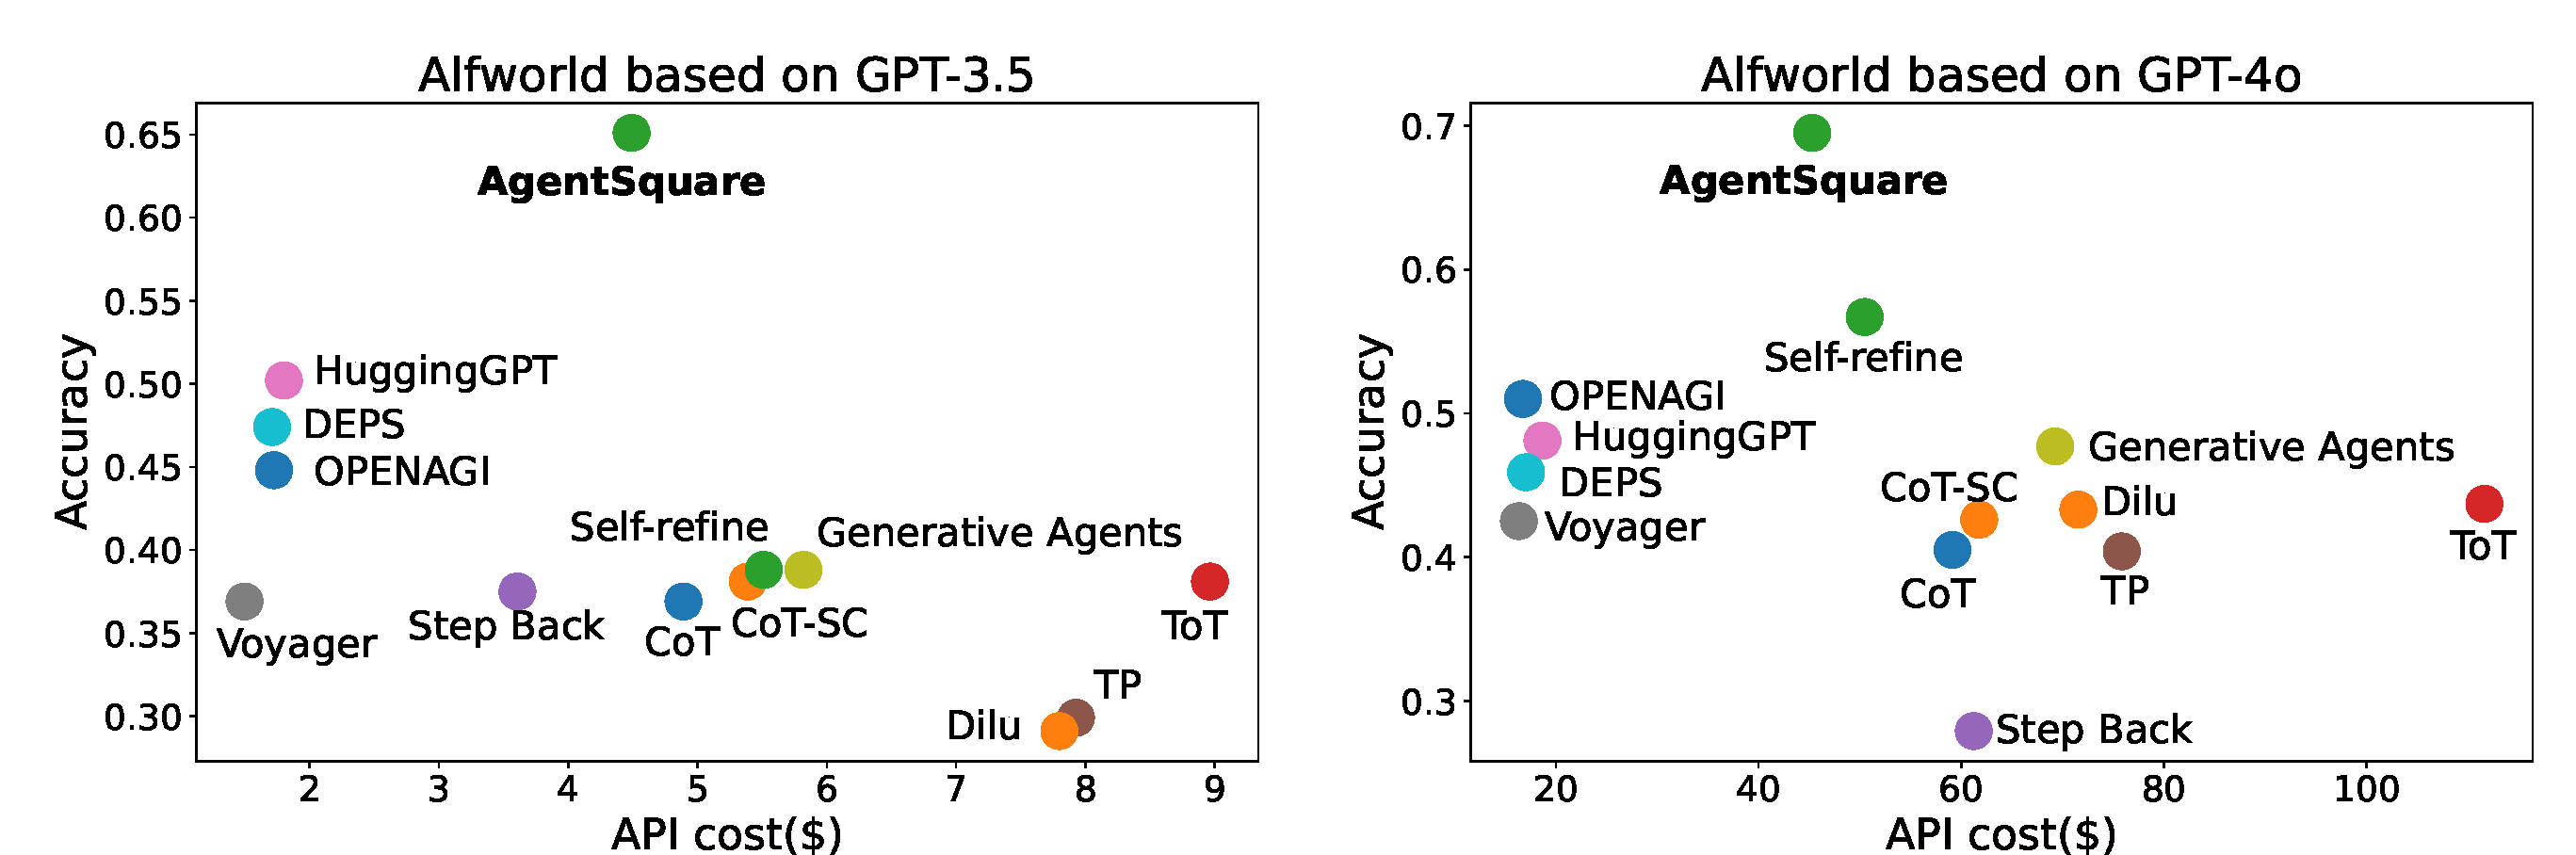
\includegraphics[width=\textwidth]{Figures/fig4_alfworld.pdf}
% \includegraphics[width=12.5cm]{Figures/f4(sci).pdf}
% \includegraphics[width=12.5cm]{Figures/f4(travel).pdf}
%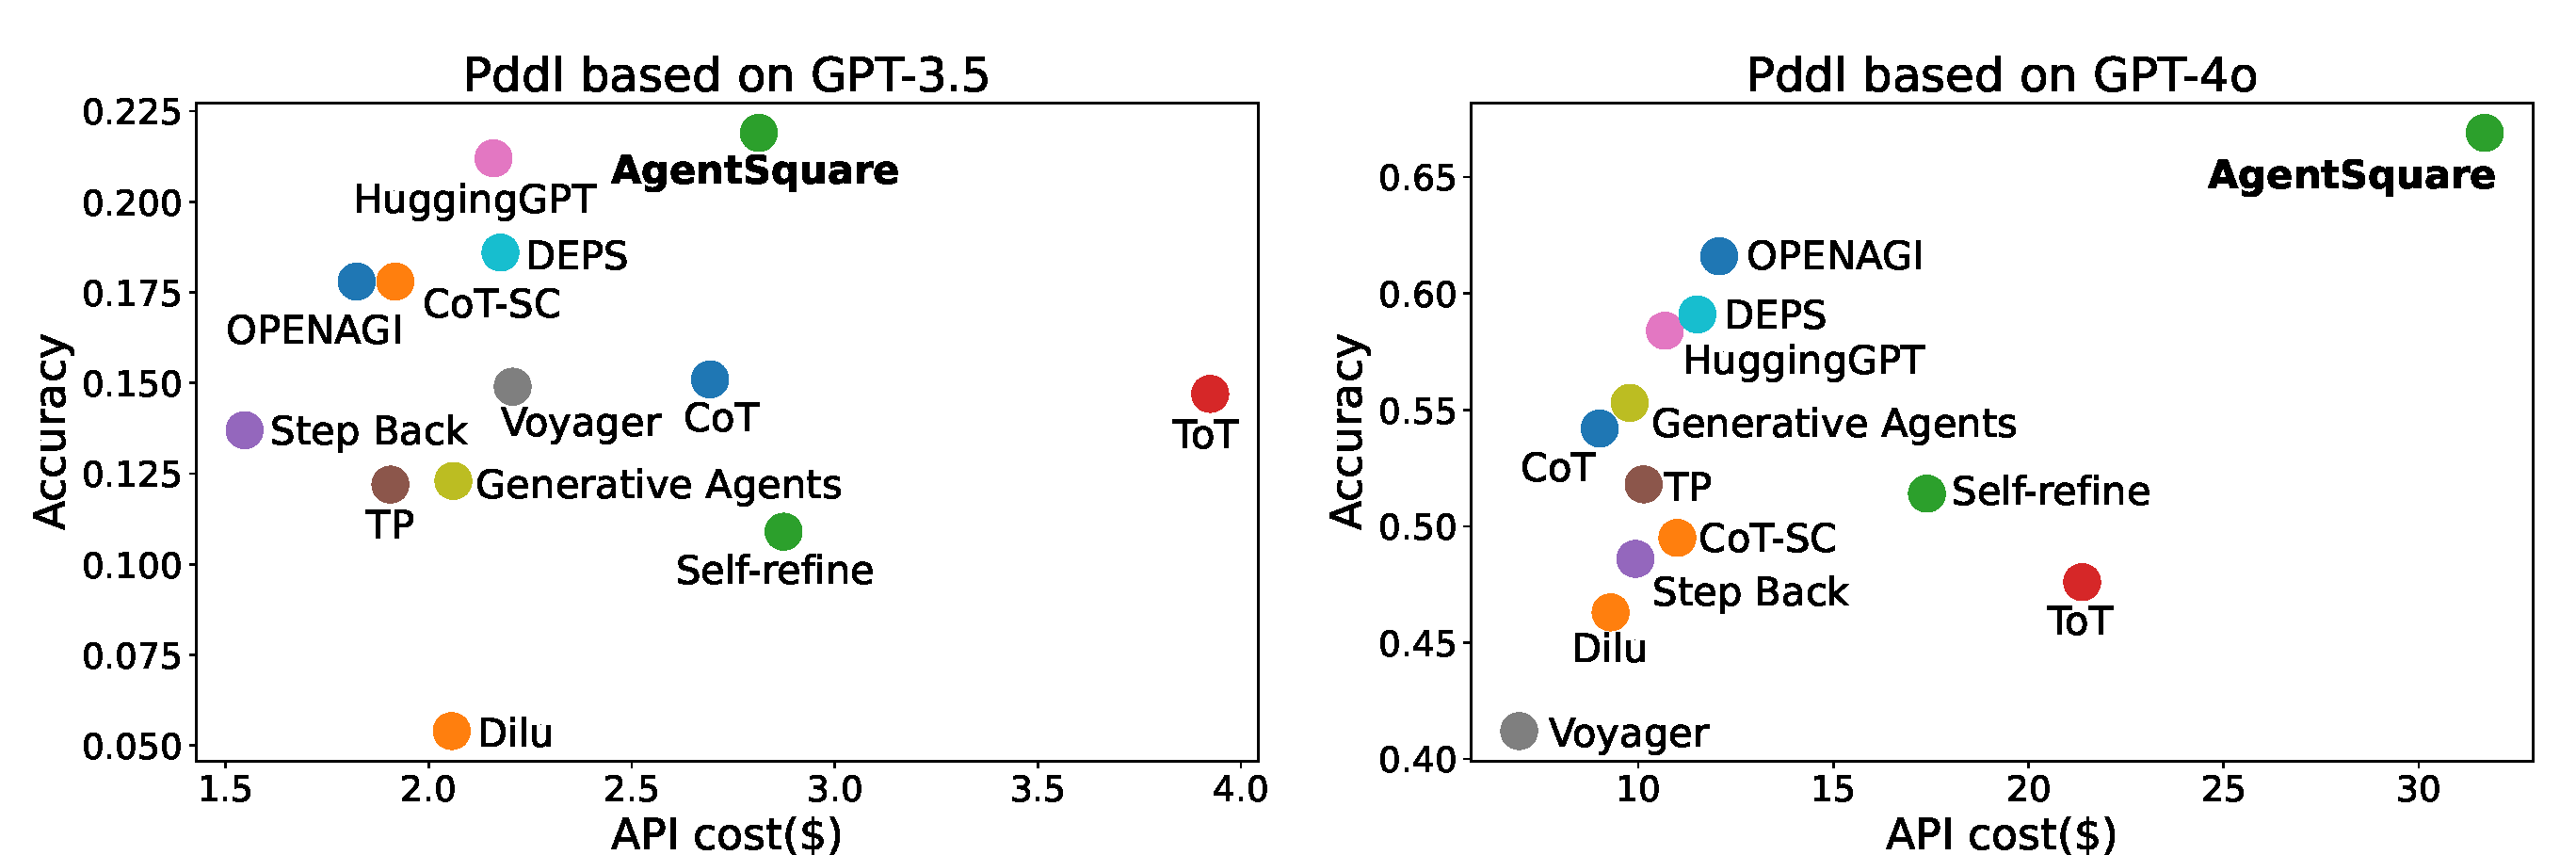
\includegraphics[width=12.5cm]{Figures/fig4_pddl.pdf}
\caption{Performance versus API costs visualization on ALFWorld task.}
\label{fig4:performance-cost}
\end{center}
\end{figure}

\begin{figure}[!t]
\begin{center}
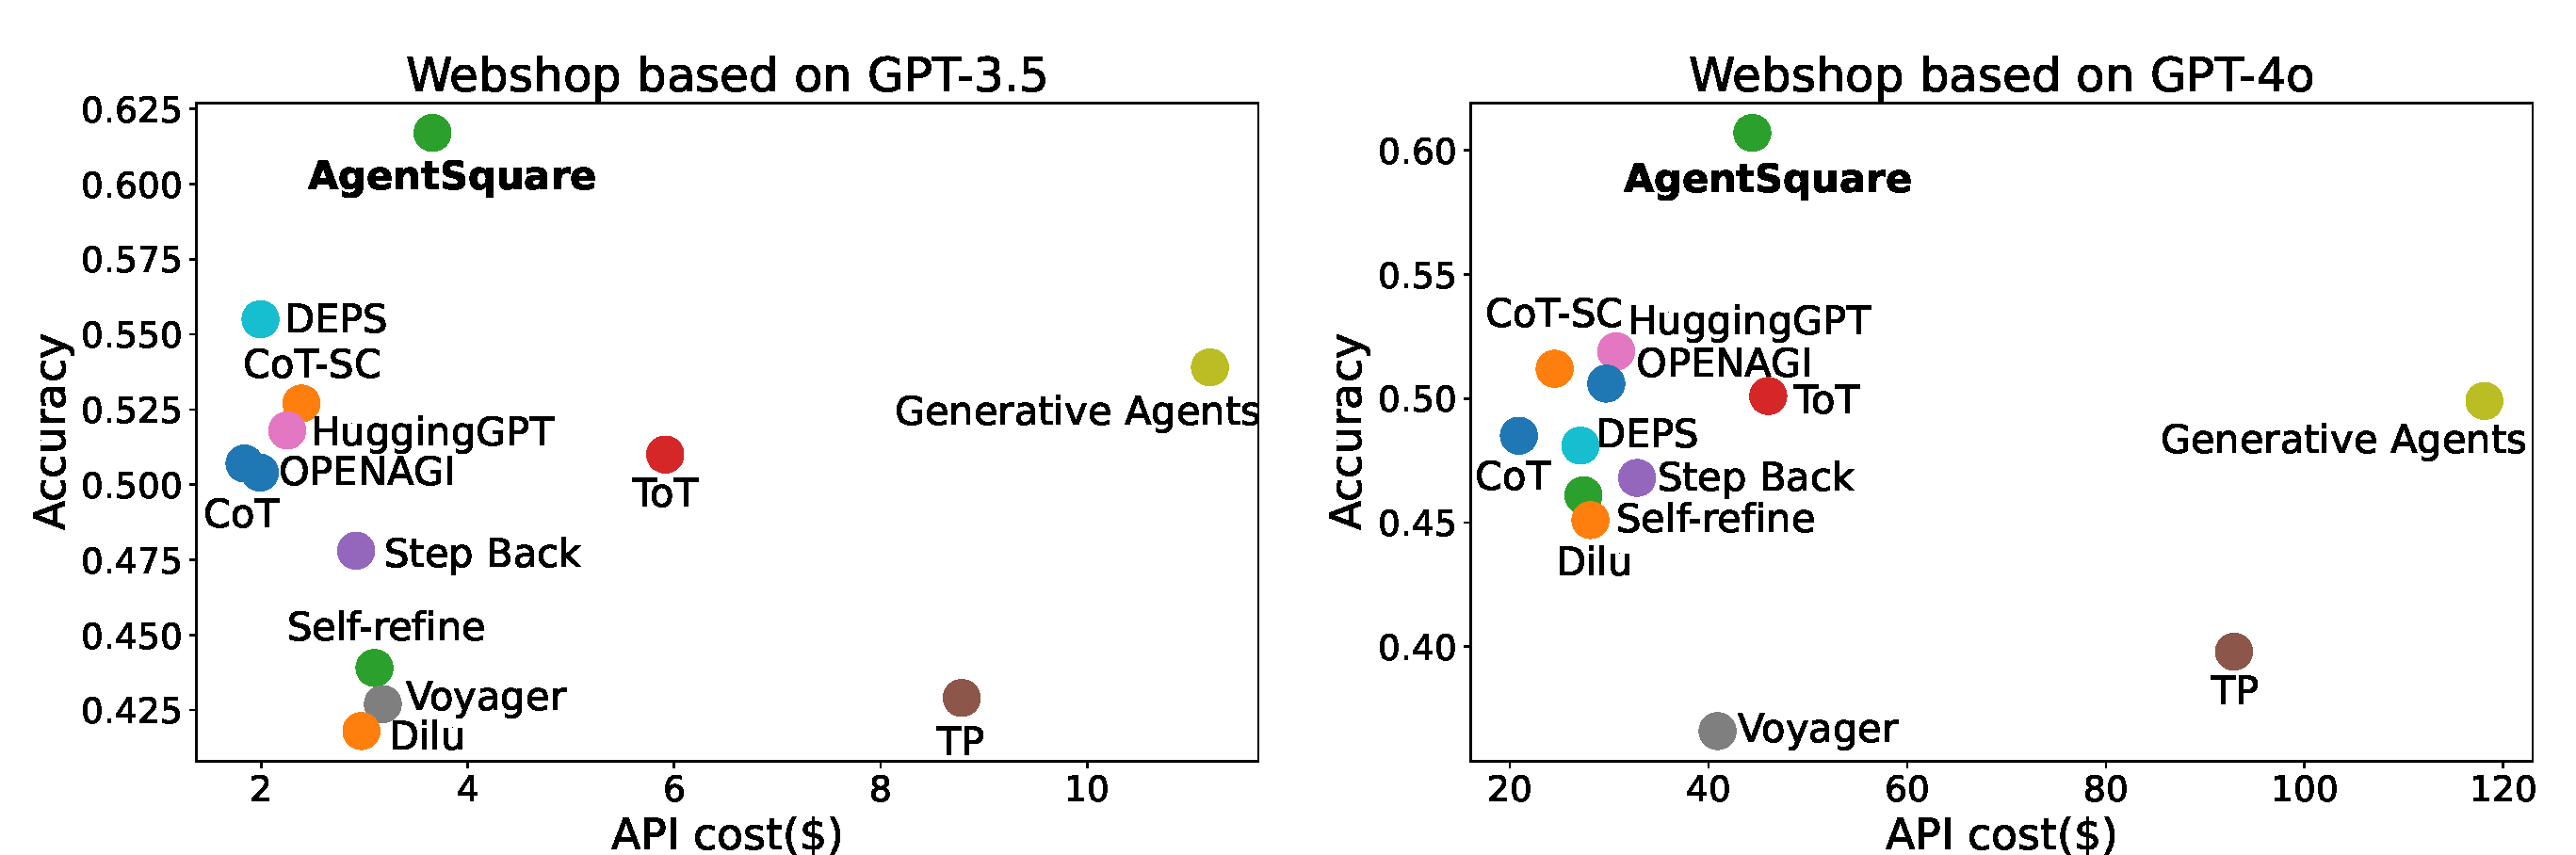
\includegraphics[width=\textwidth]{Figures/fig4_webshop.pdf}
\caption{Performance versus API costs visualization on Webshop.}
\label{app:performance-cost1}
\end{center}
\end{figure}

\begin{figure}[!t]
\begin{center}
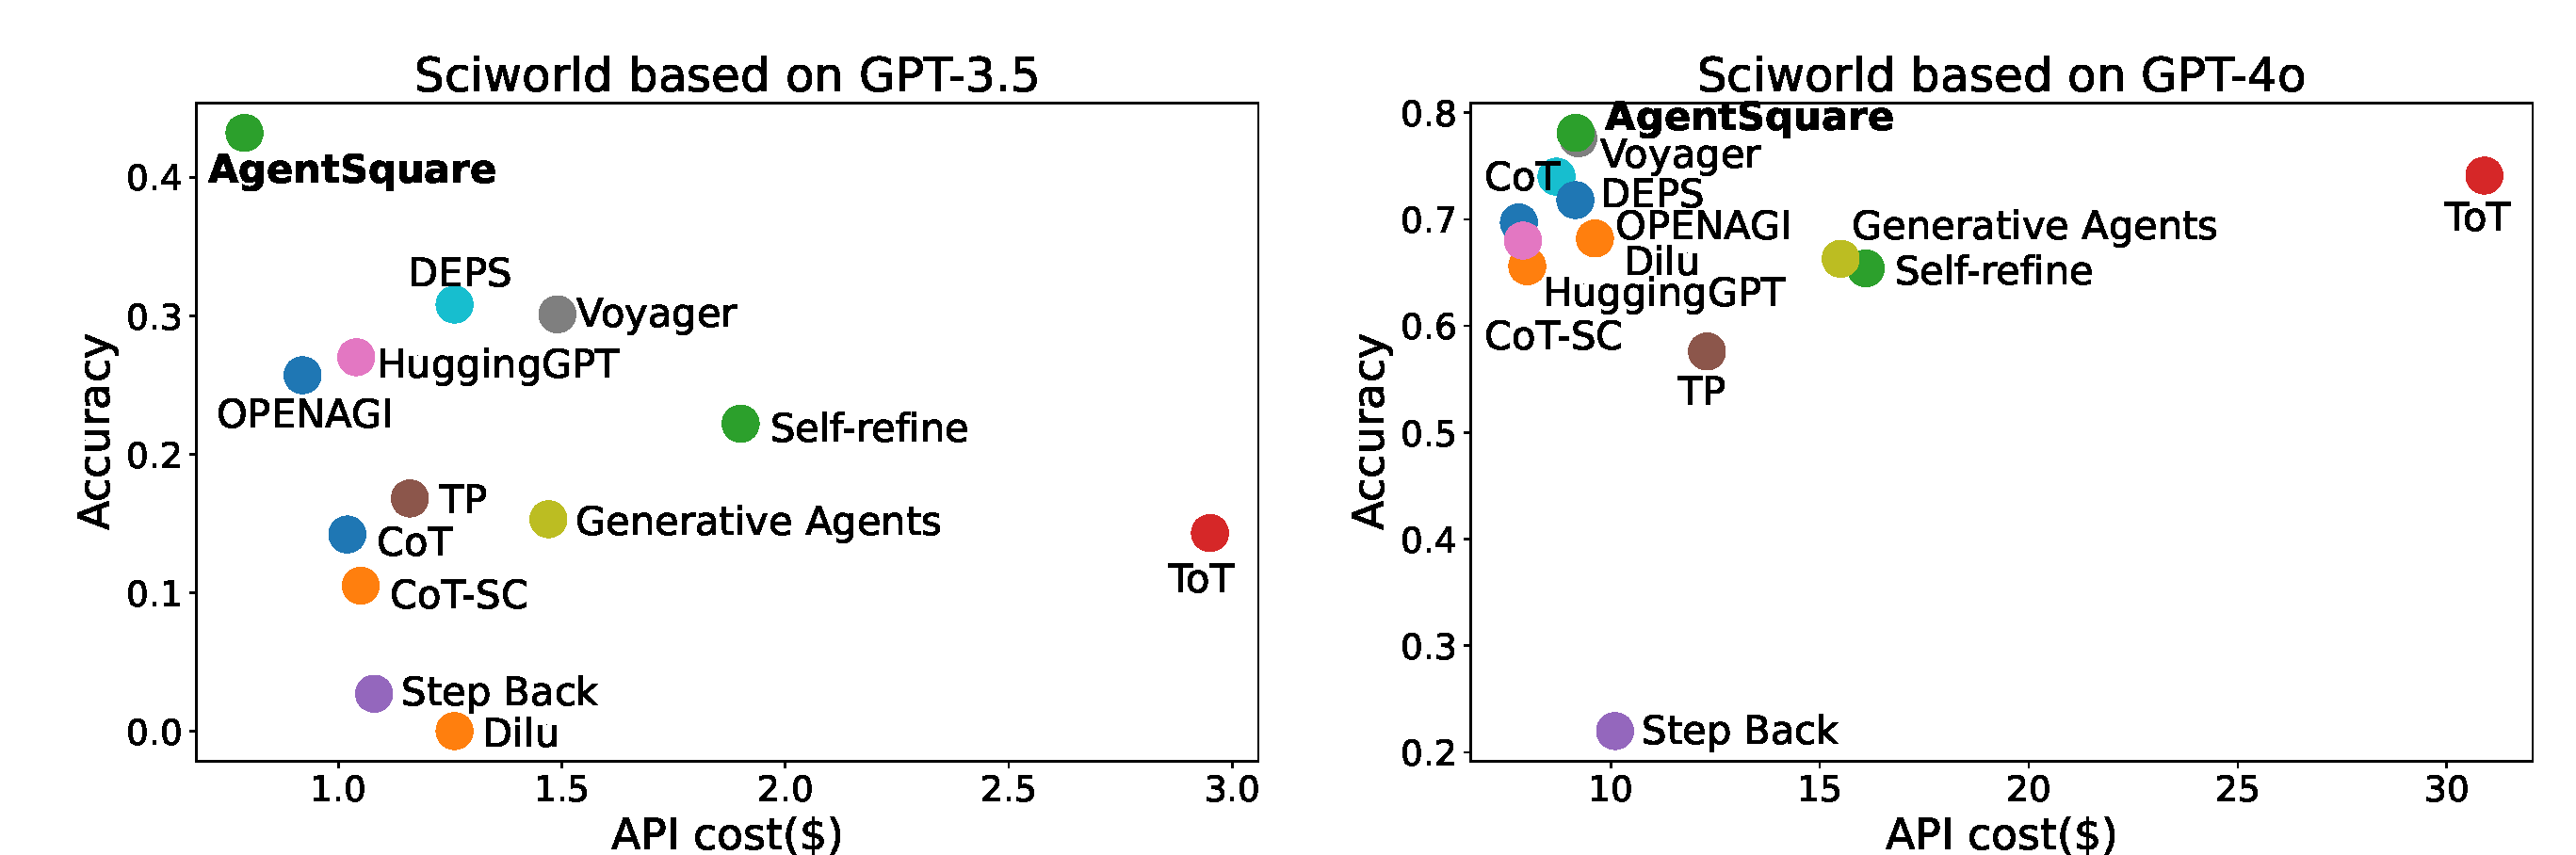
\includegraphics[width=\textwidth]{Figures/fig4_sciworld.pdf}
\caption{Performance versus API costs visualization on Sciworld.}
\label{app:performance-cost2}
\end{center}
\end{figure}

\begin{figure}[!t]
\begin{center}
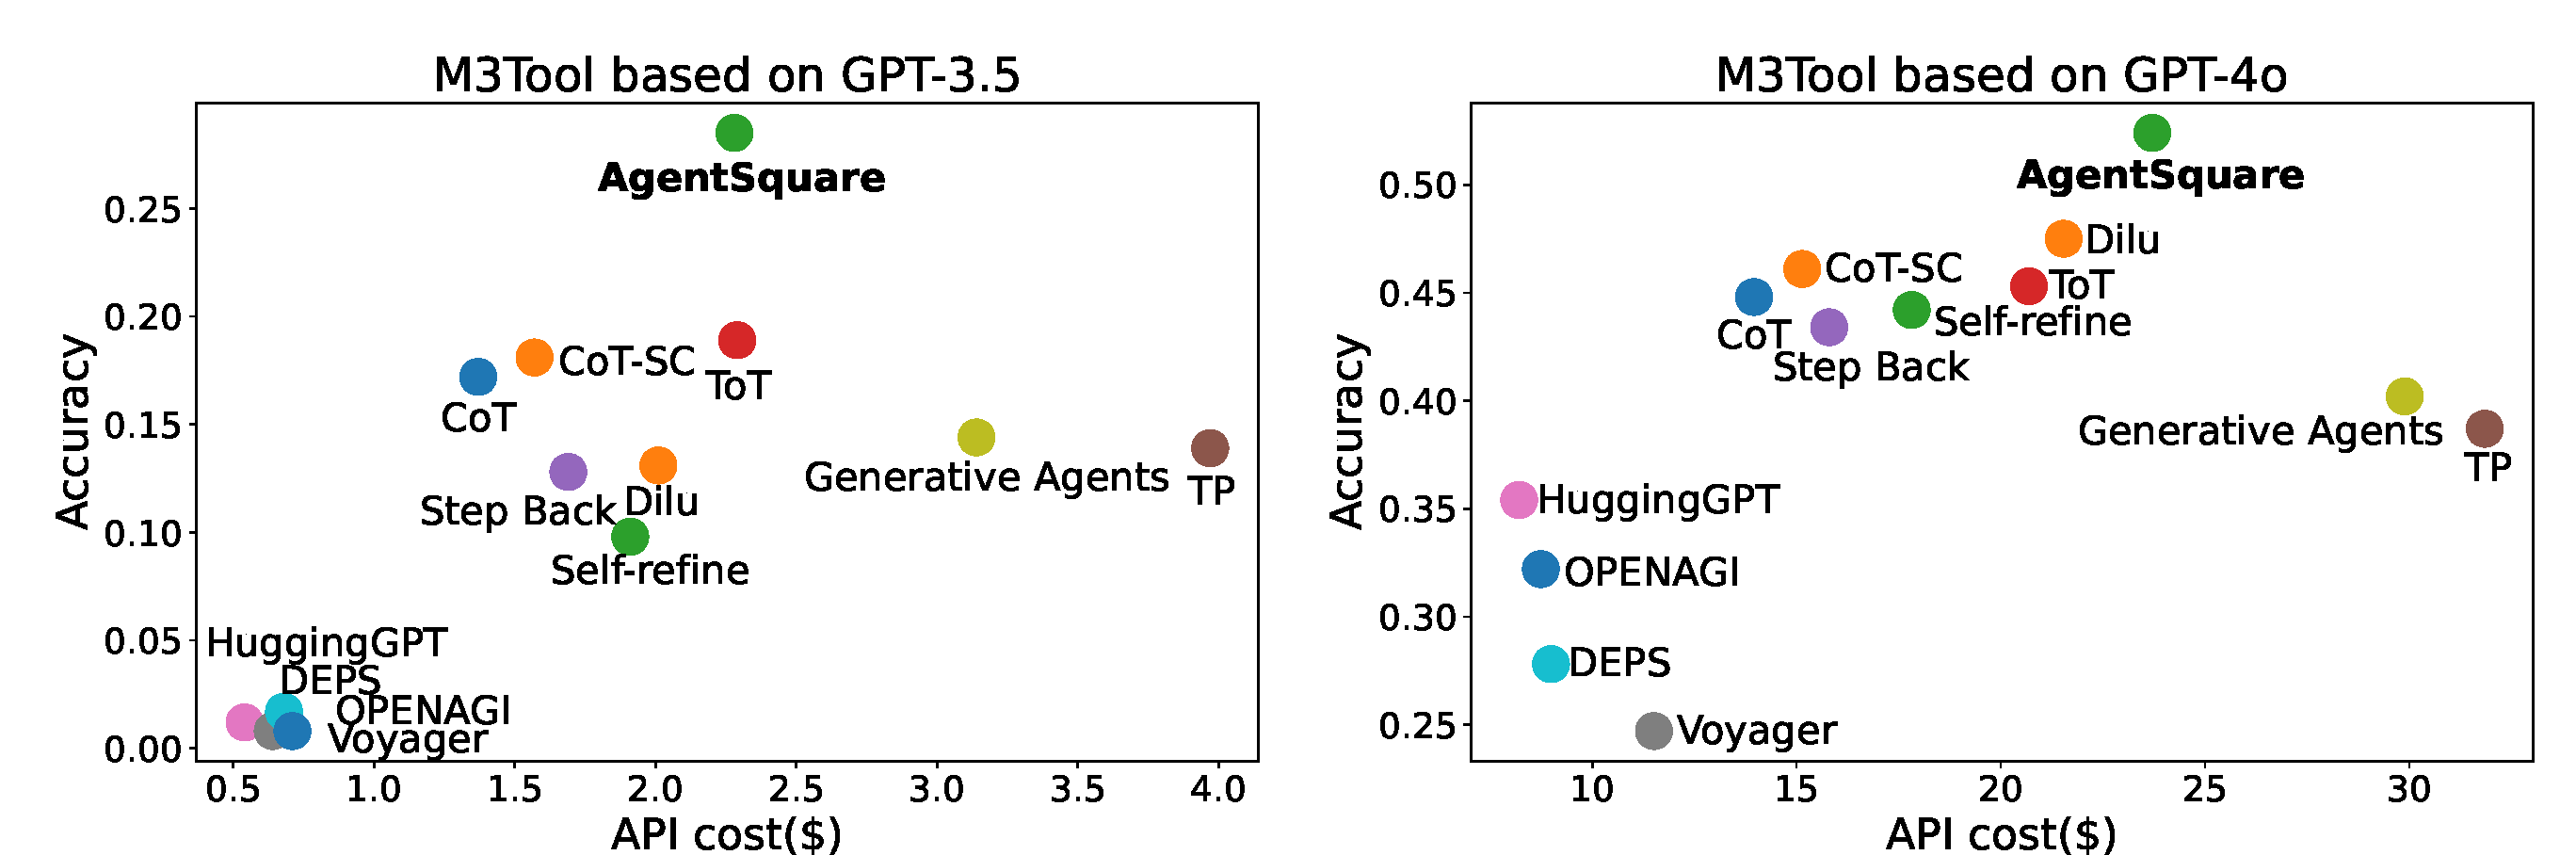
\includegraphics[width=\textwidth]{Figures/fig4_m3tool.pdf}
\caption{Performance versus API costs visualization on M3tool.}
\label{app:performance-cost3}
\end{center}
\end{figure}

\begin{figure}[!t]
\begin{center}
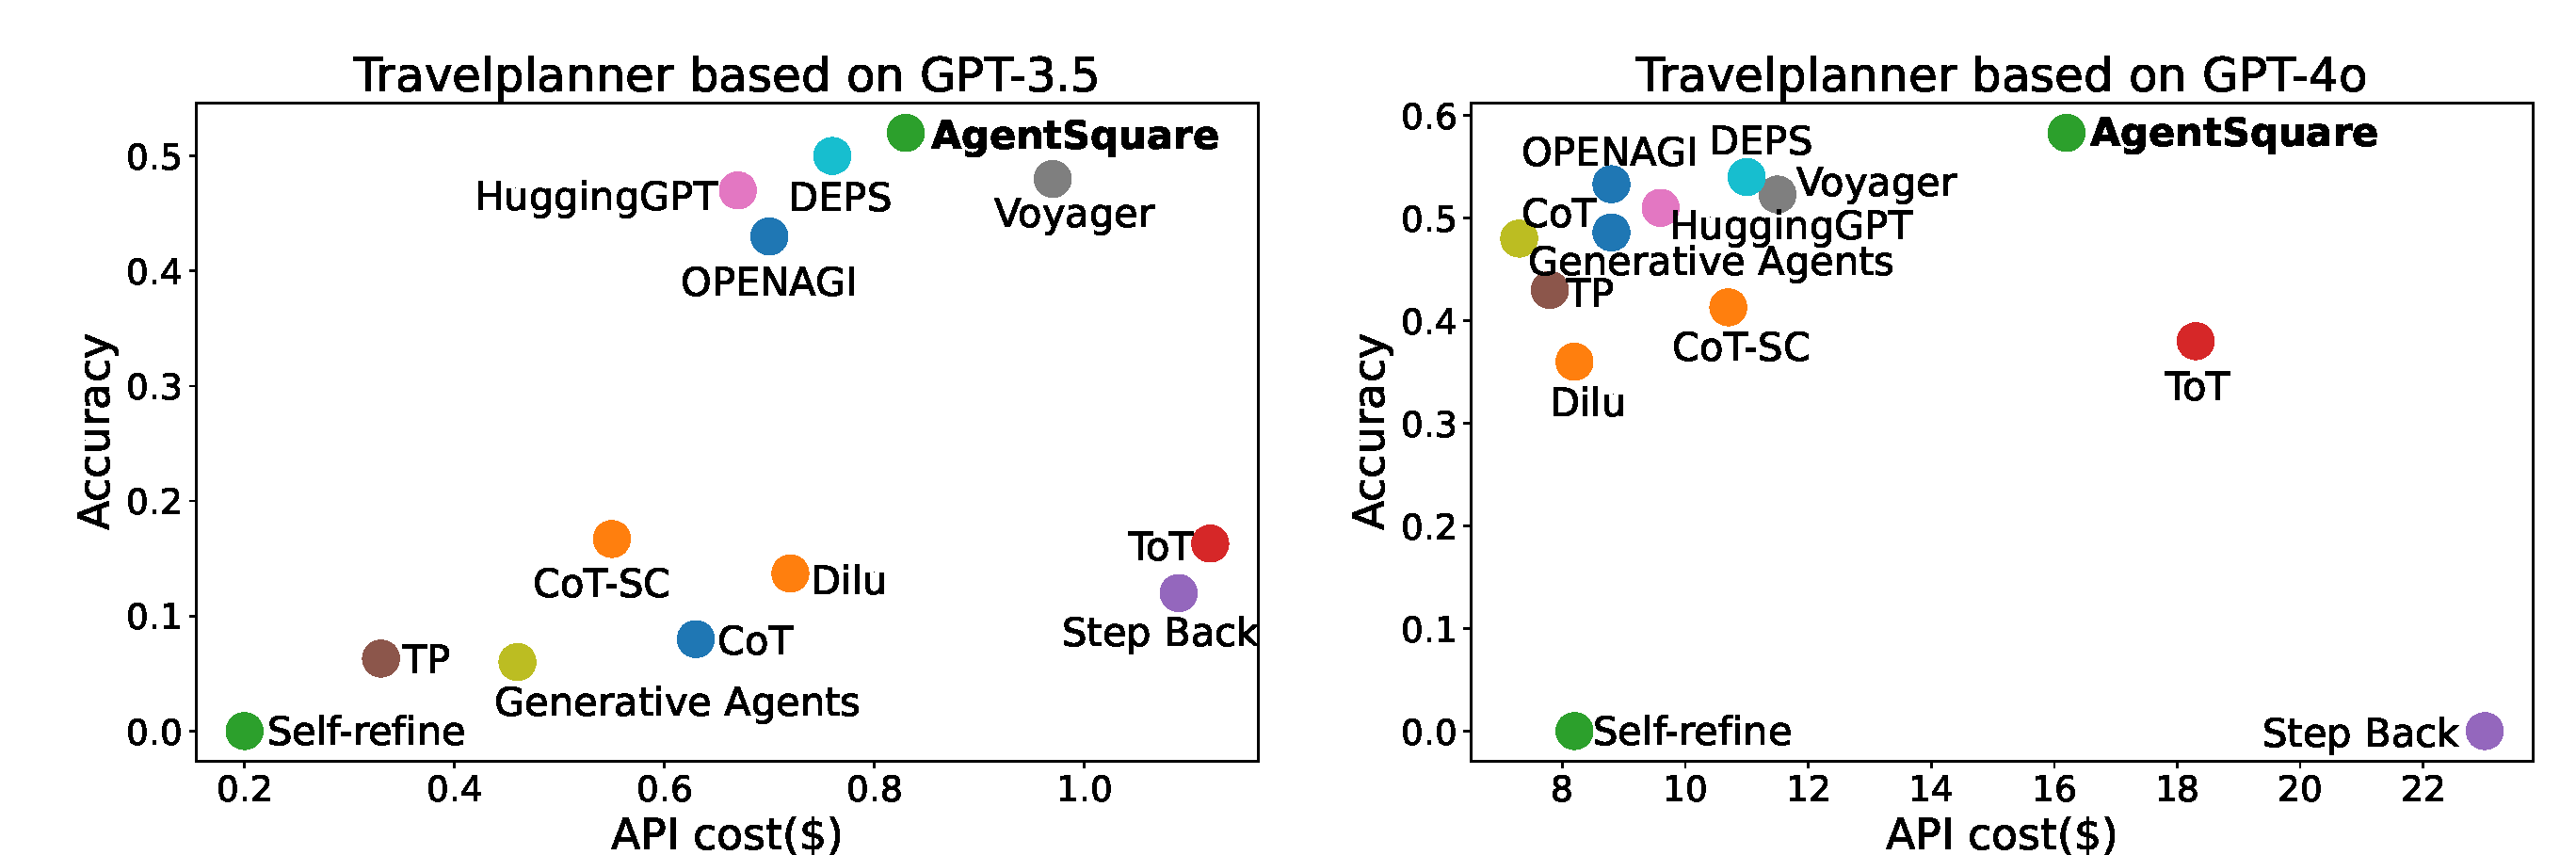
\includegraphics[width=\textwidth]{Figures/fig4_travelplanner.pdf}
\caption{Performance versus API costs visualization on Travelplanner.}
\label{app:performance-cost4}
\end{center}
\end{figure}

\begin{figure}[!t]
\begin{center}
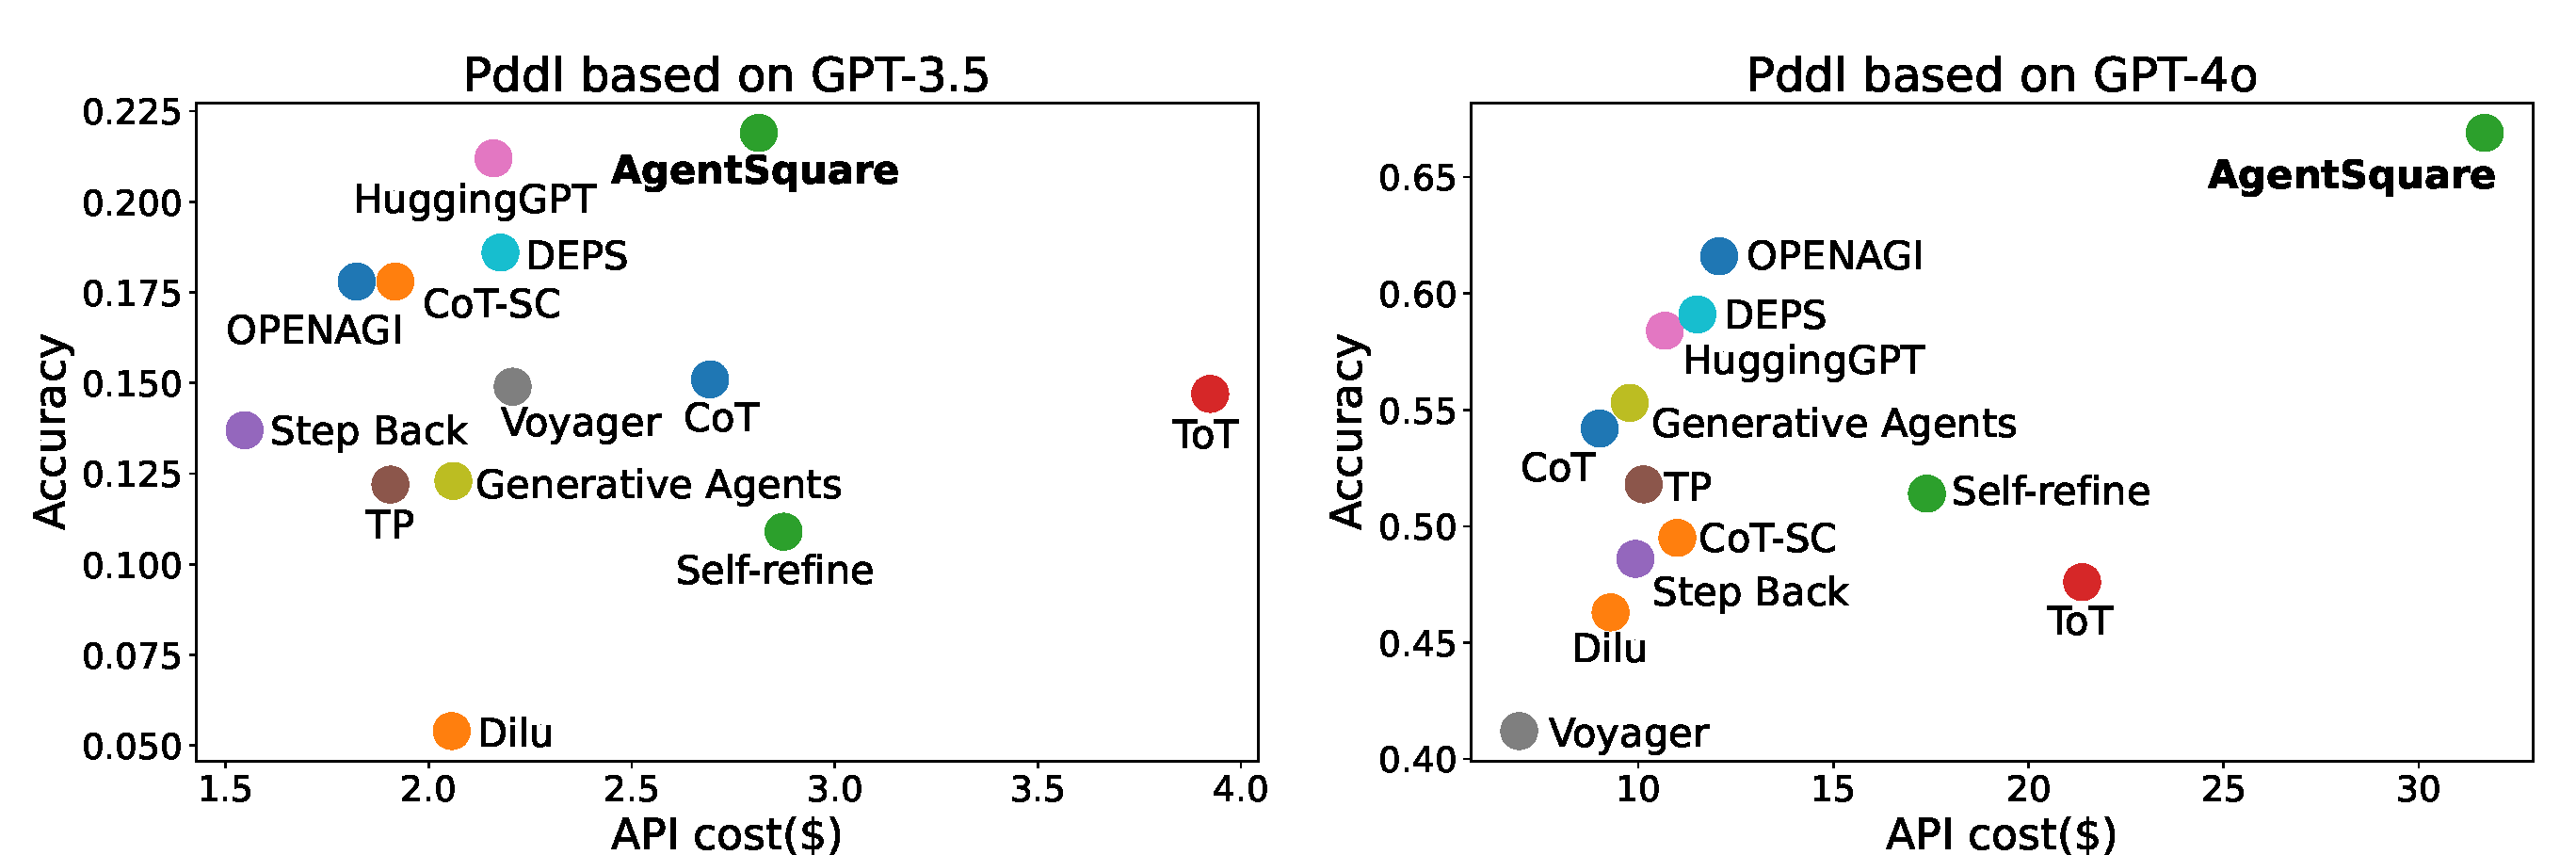
\includegraphics[width=\textwidth]{Figures/fig4_pddl.pdf}
\caption{Performance versus API costs visualization on PDDL.}
\label{app:performance-cost5}
\end{center}
\end{figure}

\begin{figure}[!t]
\begin{center}
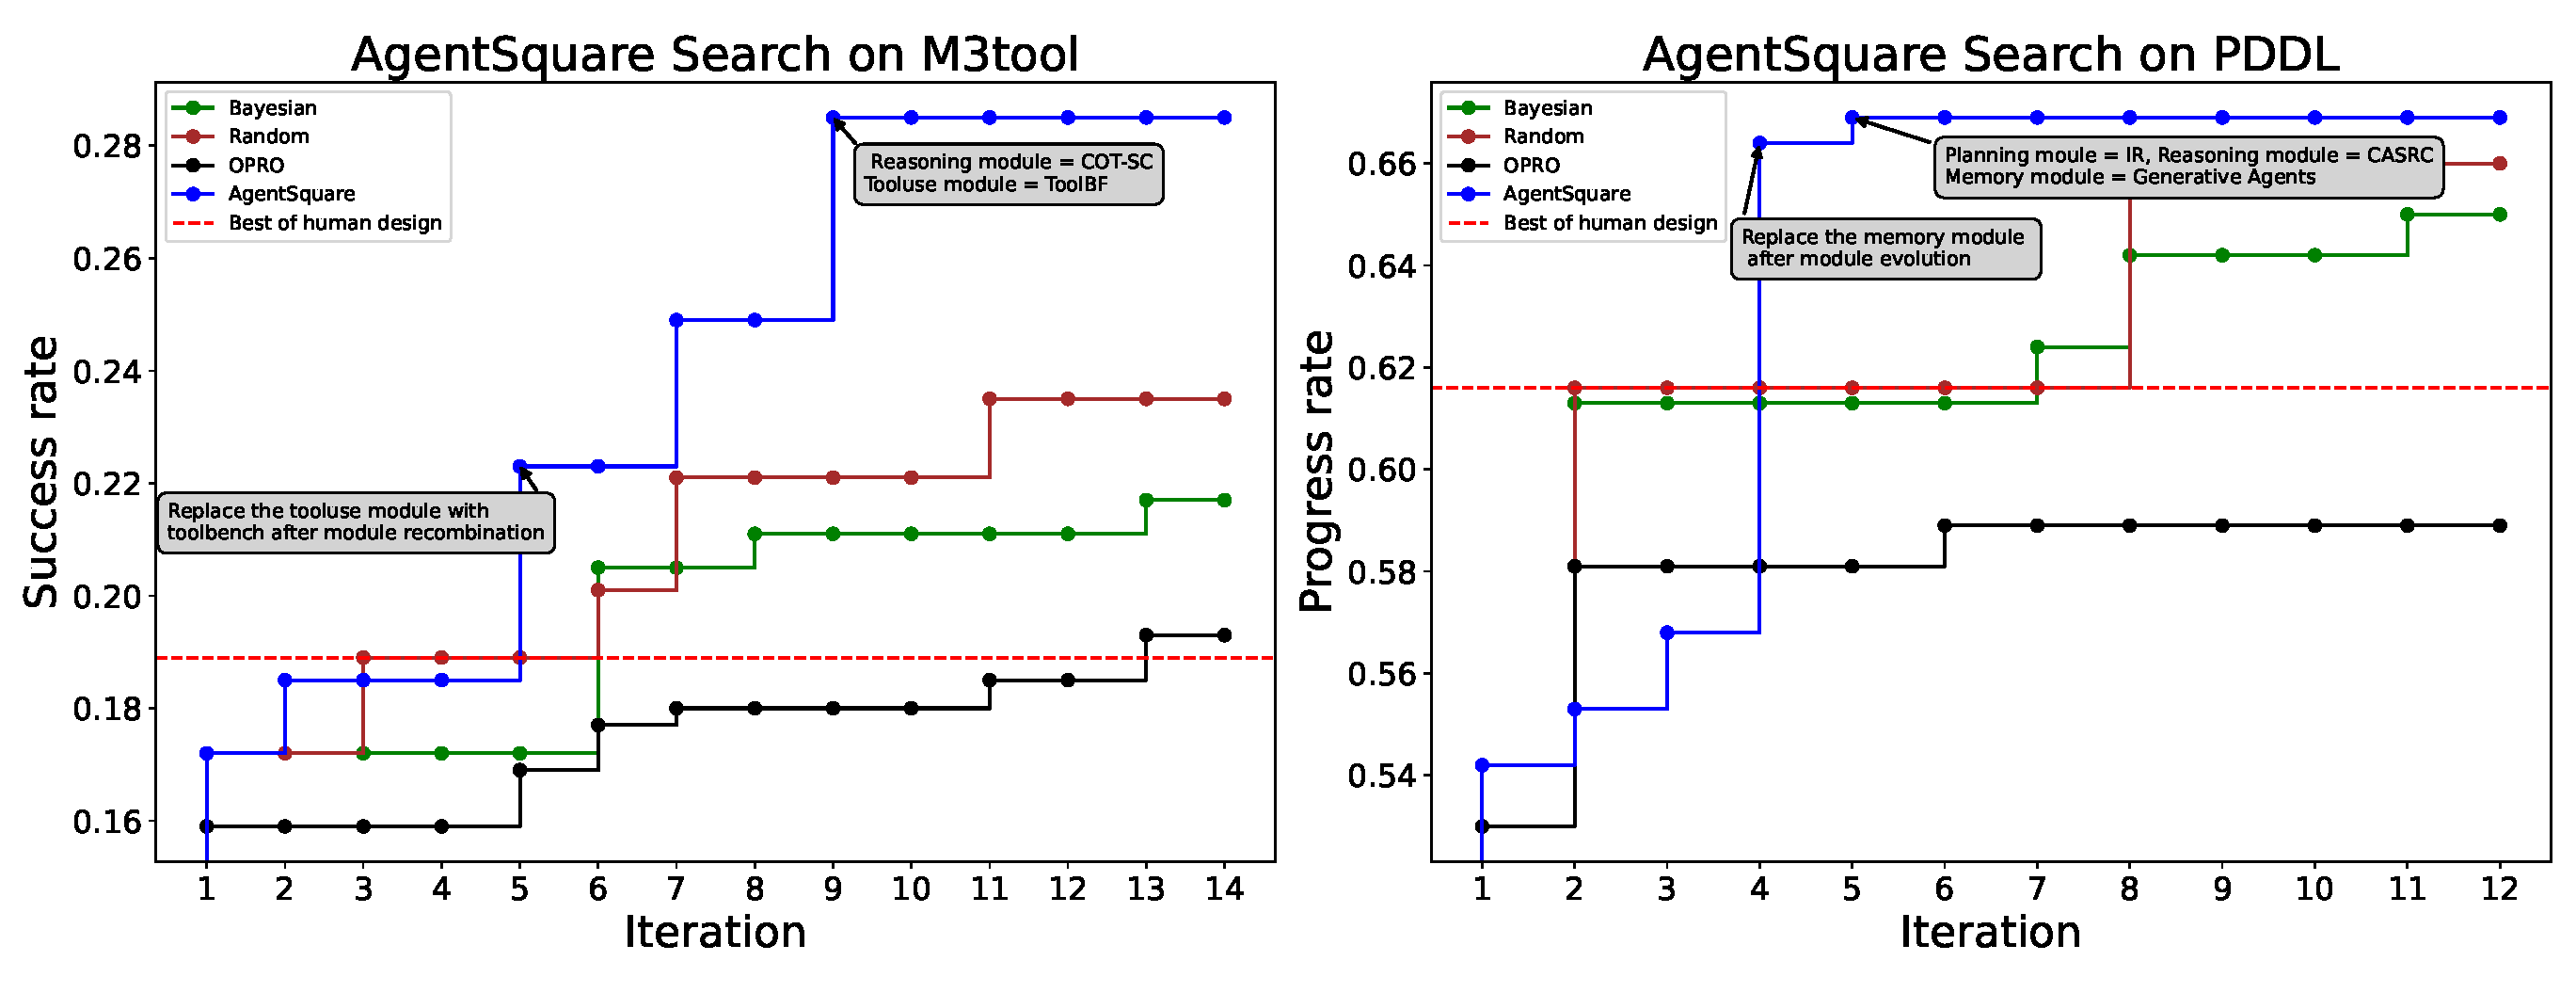
\includegraphics[width=\textwidth]{Figures/fig5_m3tool_pddl.pdf}
\caption{AgentSquare search trajectory on M3tool and PDDL (more hand-crafted agents, specific module combinations when surpassing best hand-crafted and the final evolved agent, other search baselines).}
\label{app:trajectory1}
\end{center}
\end{figure}

\begin{figure}[!t]
\begin{center}
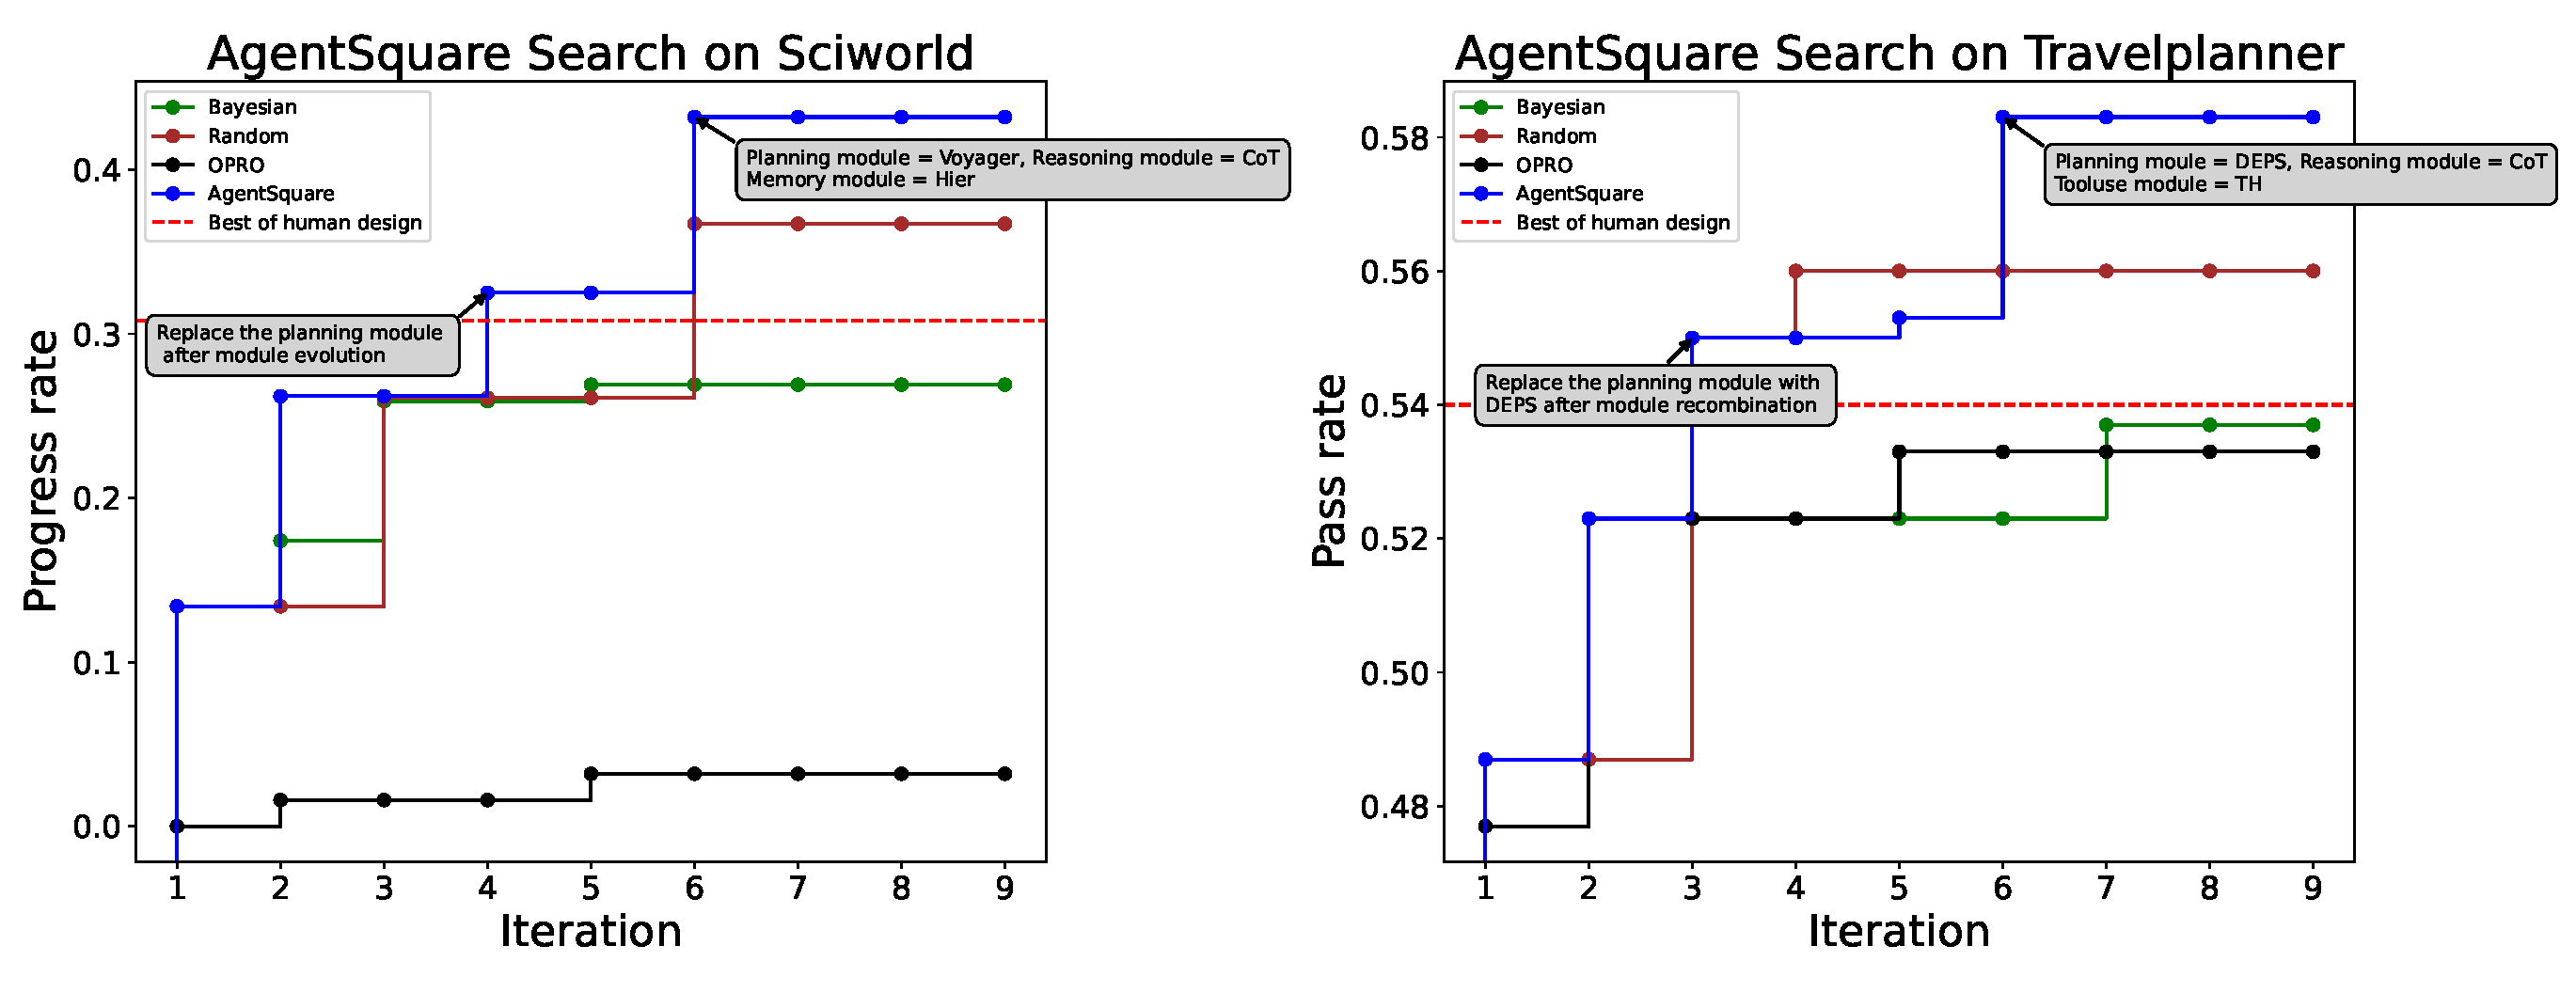
\includegraphics[width=\textwidth]{Figures/fig5_sciworld_travelplanner.pdf}
\caption{AgentSquare search trajectory on Sciworld and Travelplanner (more hand-crafted agents, specific module combinations when surpassing best hand-crafted and the final evolved agent, other search baselines).}
\label{app:trajectory2}
\end{center}
\end{figure}

\begin{figure}[!t]
\begin{center}
%\fbox{\rule[-.5cm]{0cm}{4cm} \rule[-.5cm]{4cm}{0cm}}
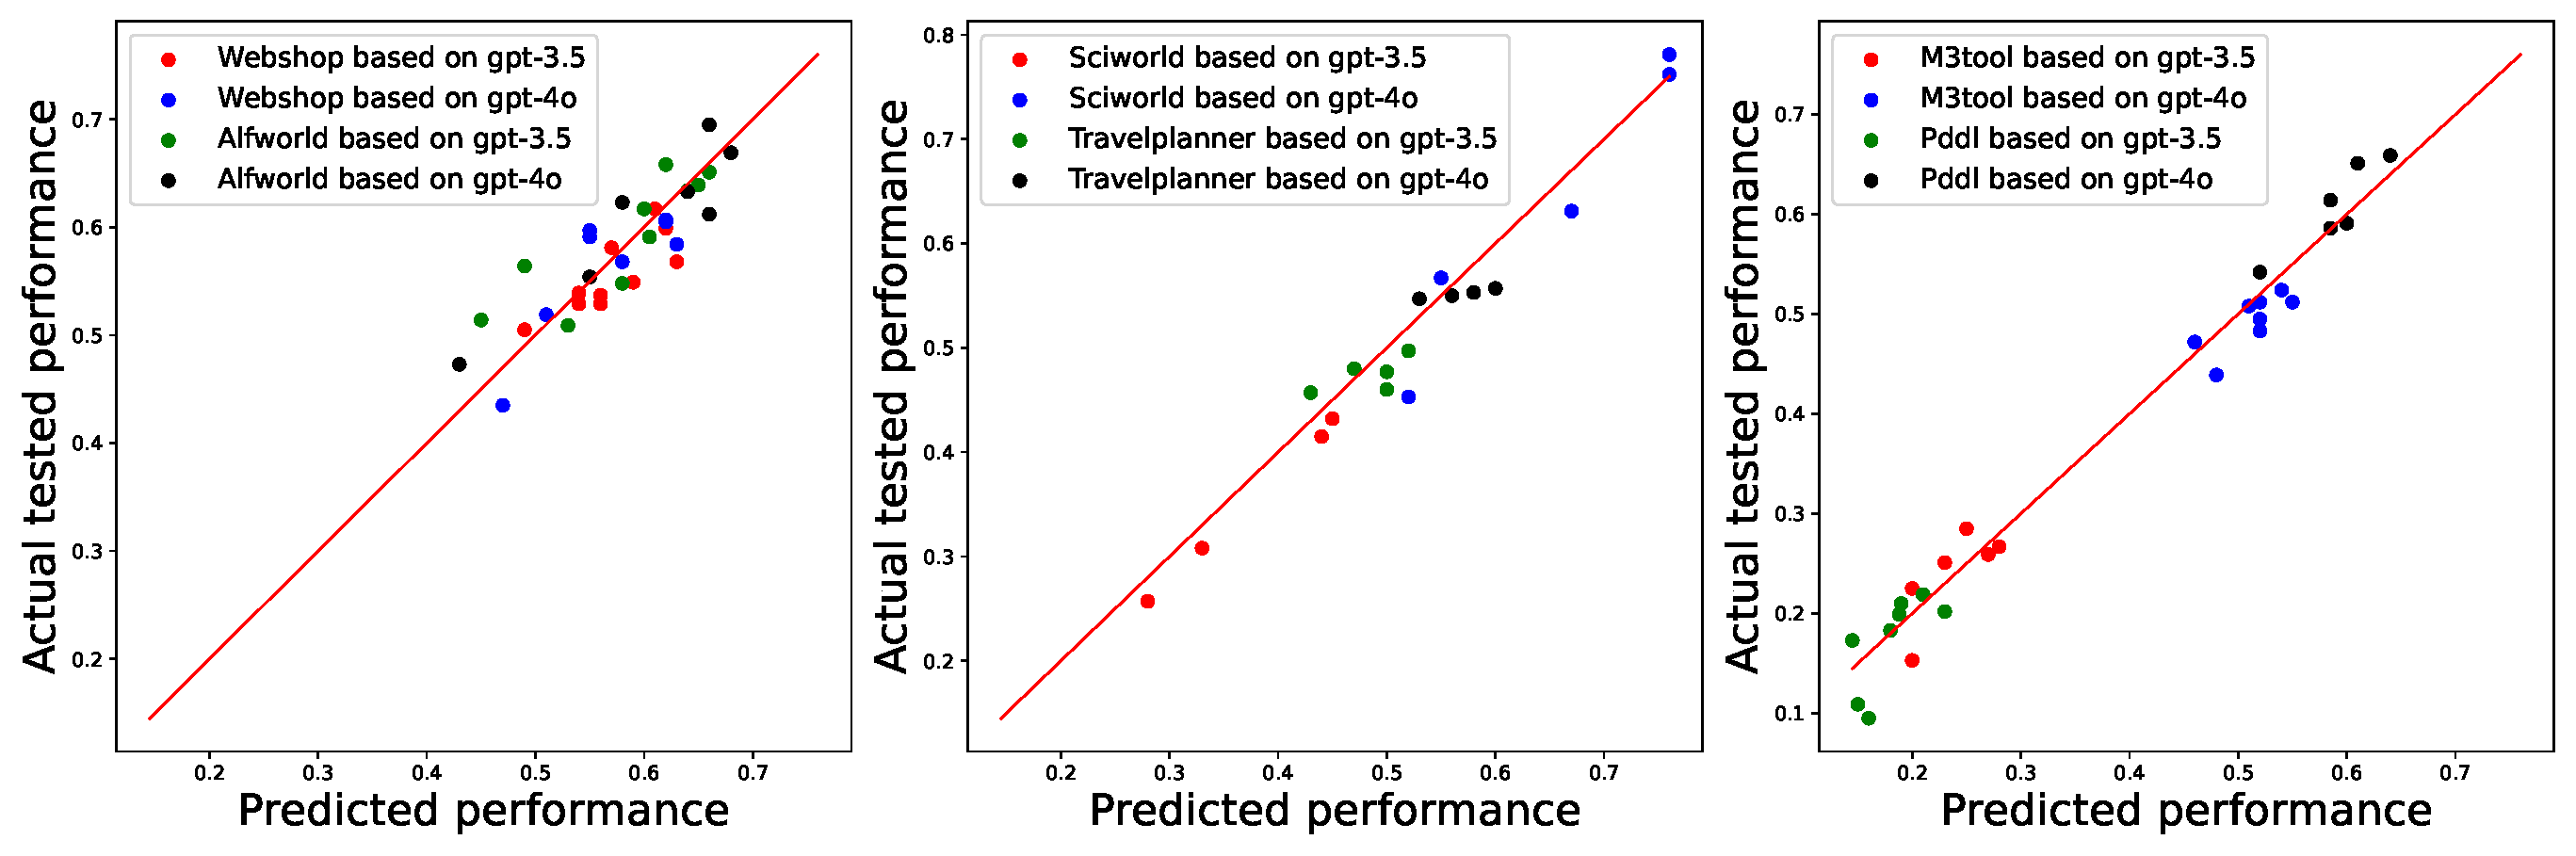
\includegraphics[width=0.85\textwidth]{Figures/fig5-more_data_points.pdf}
\caption{Validation of the effectiveness of the performance predictor on dynamically searched agents for each task.}
\label{pp-search}
\end{center}
\end{figure}

% \begin{figure}[h]
% \begin{center}
% 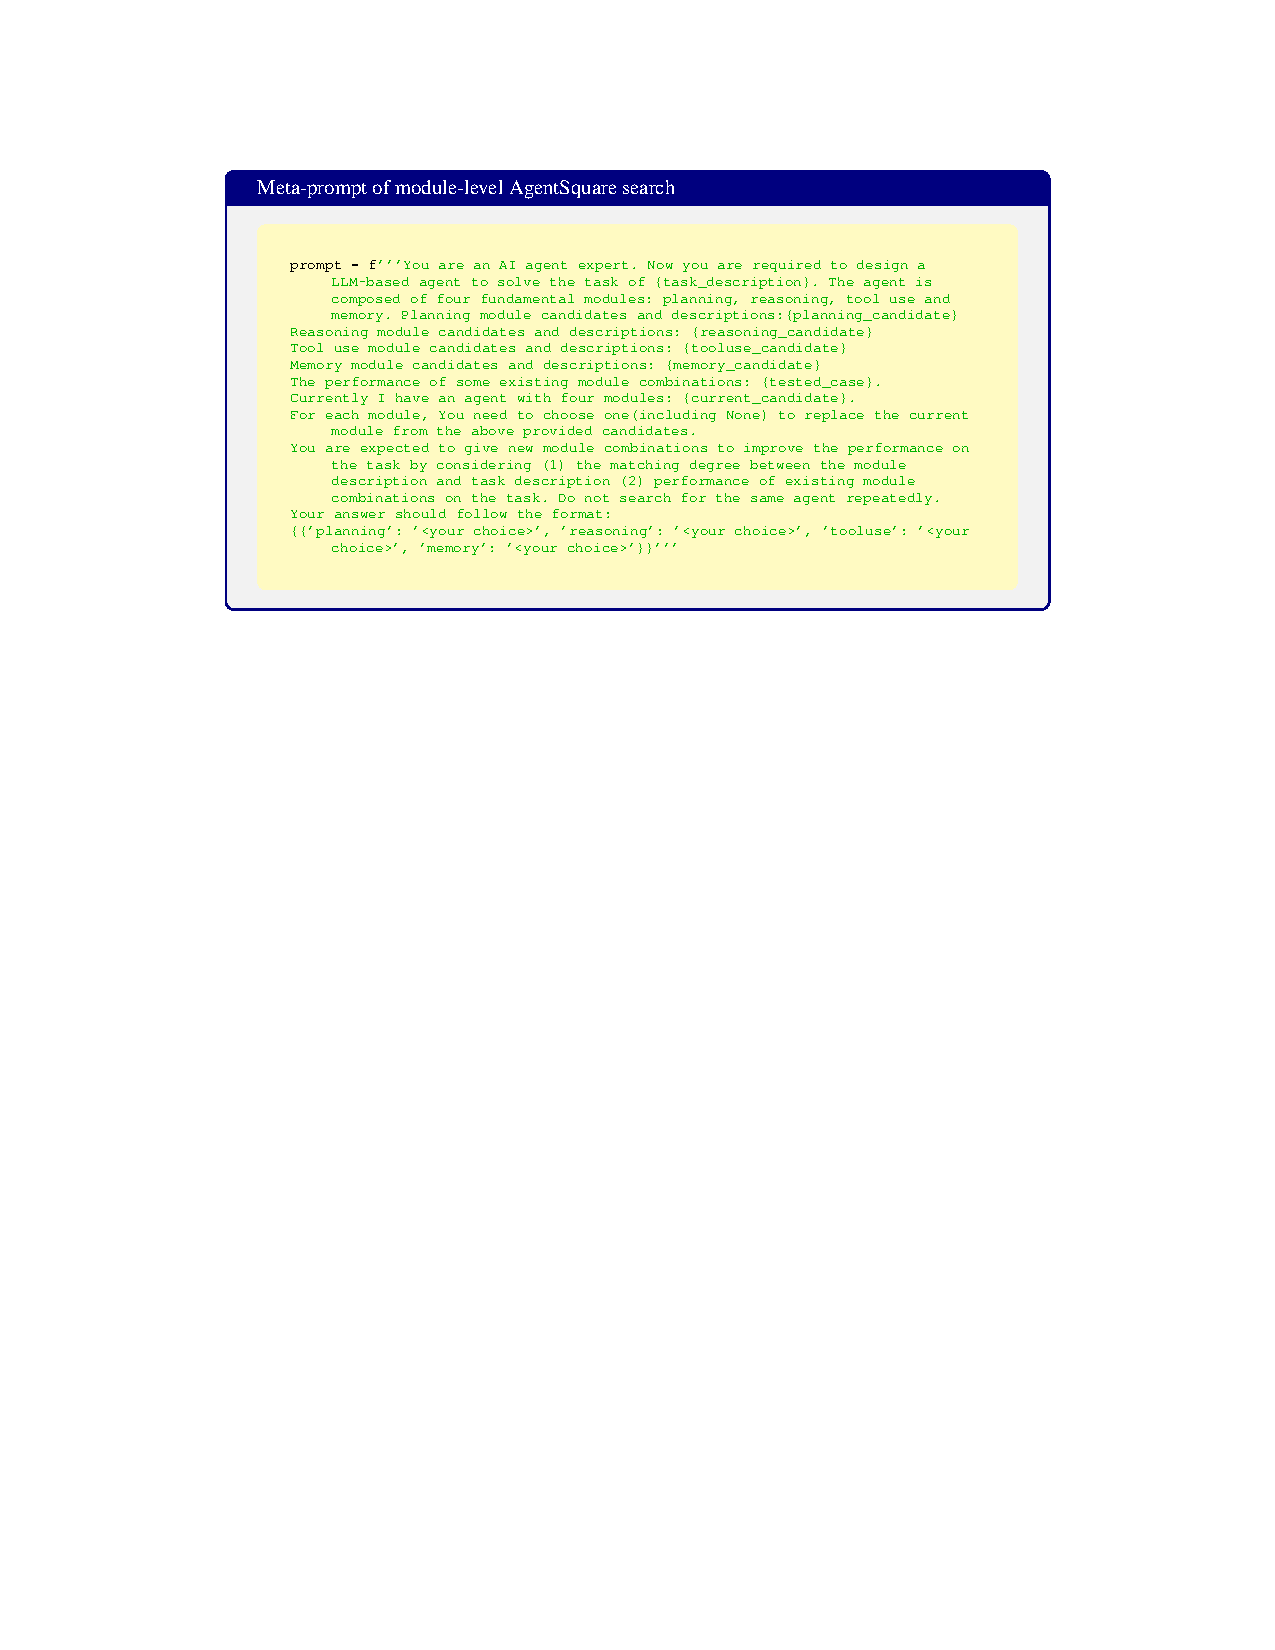
\includegraphics[width=\textwidth]{Figures/prompt_module_search.pdf}
% \caption{Meta-prompt of module recombination in AgentSquare search.}
% \label{app:module-level1}
% \end{center}
% \end{figure}

% \begin{figure}[h]
% \begin{center}
% 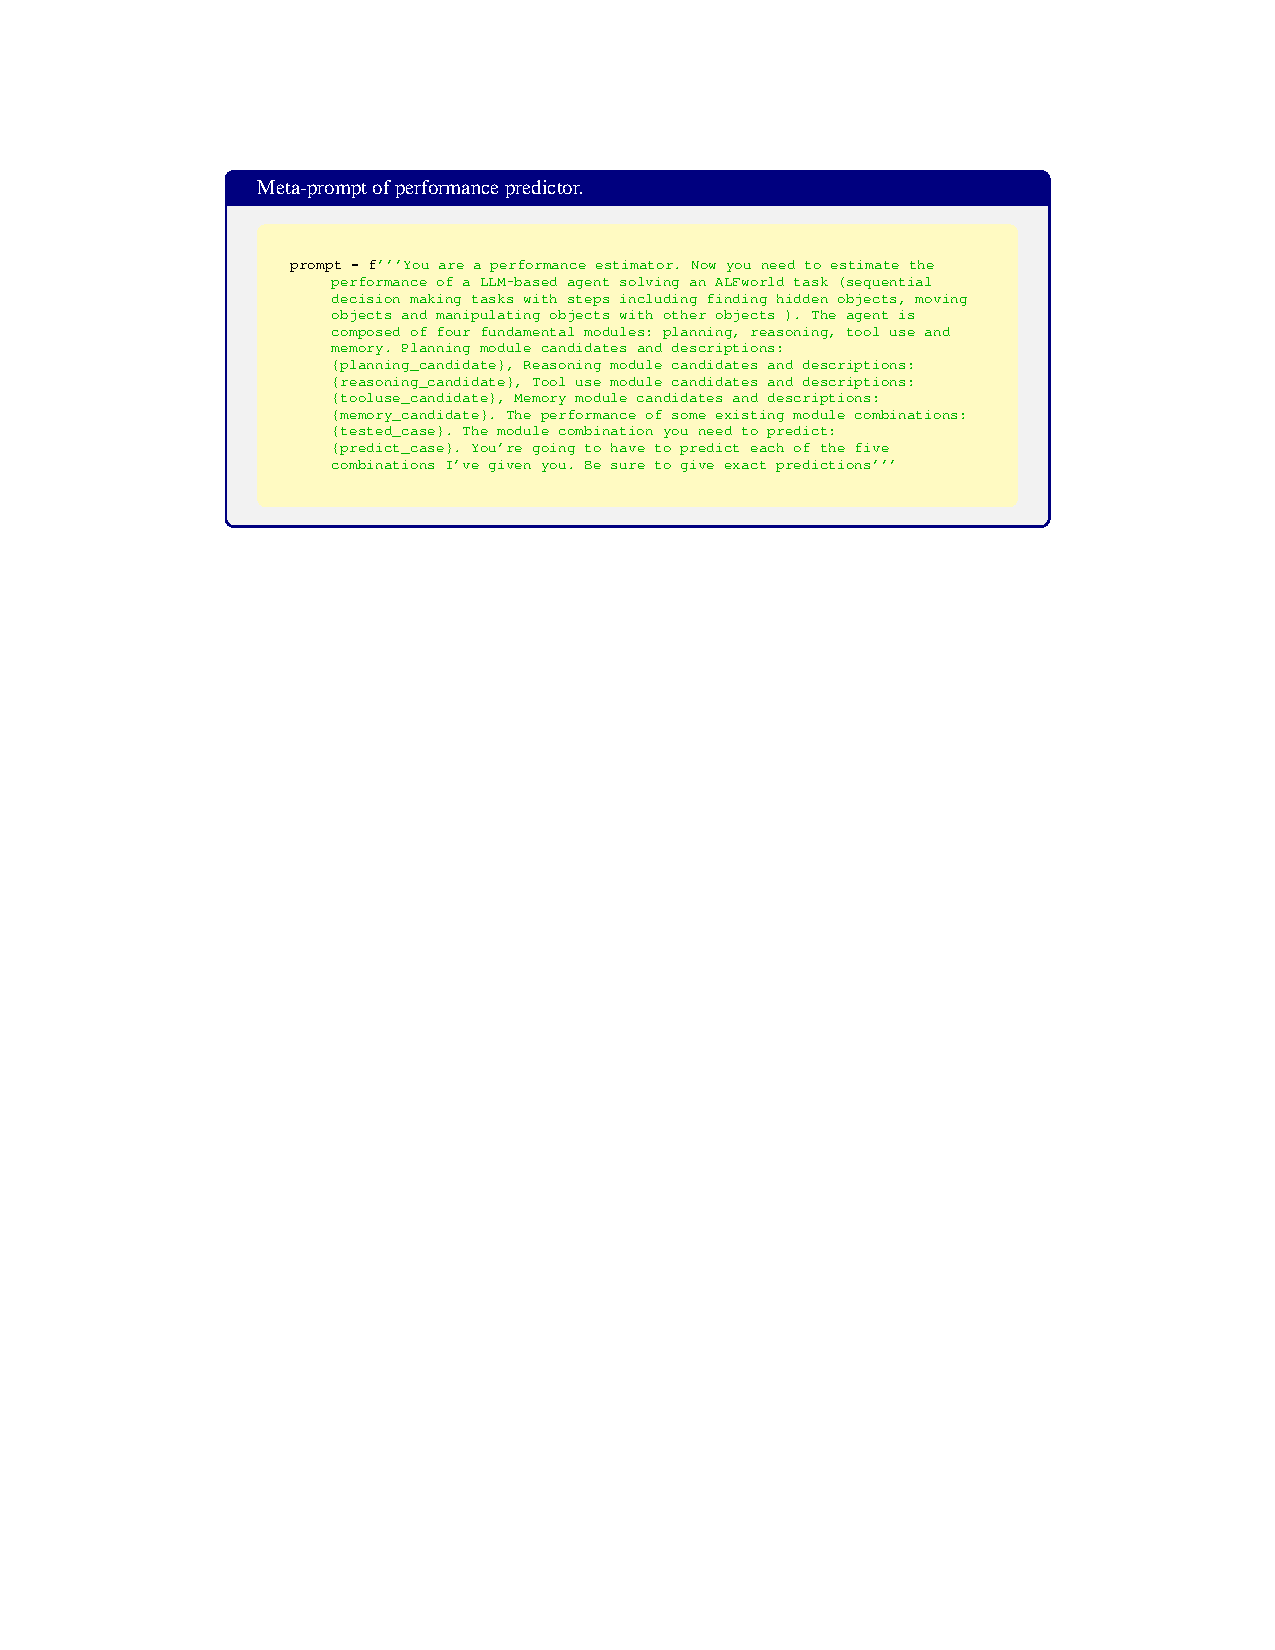
\includegraphics[width=\textwidth]{Figures/prompt_performance_predictor.pdf}
% \caption{Meta-prompt of performance predictor.}
% \label{app:pp-prompt}
% \end{center}
% \end{figure}

% \begin{figure}[h]
% \begin{center}
% 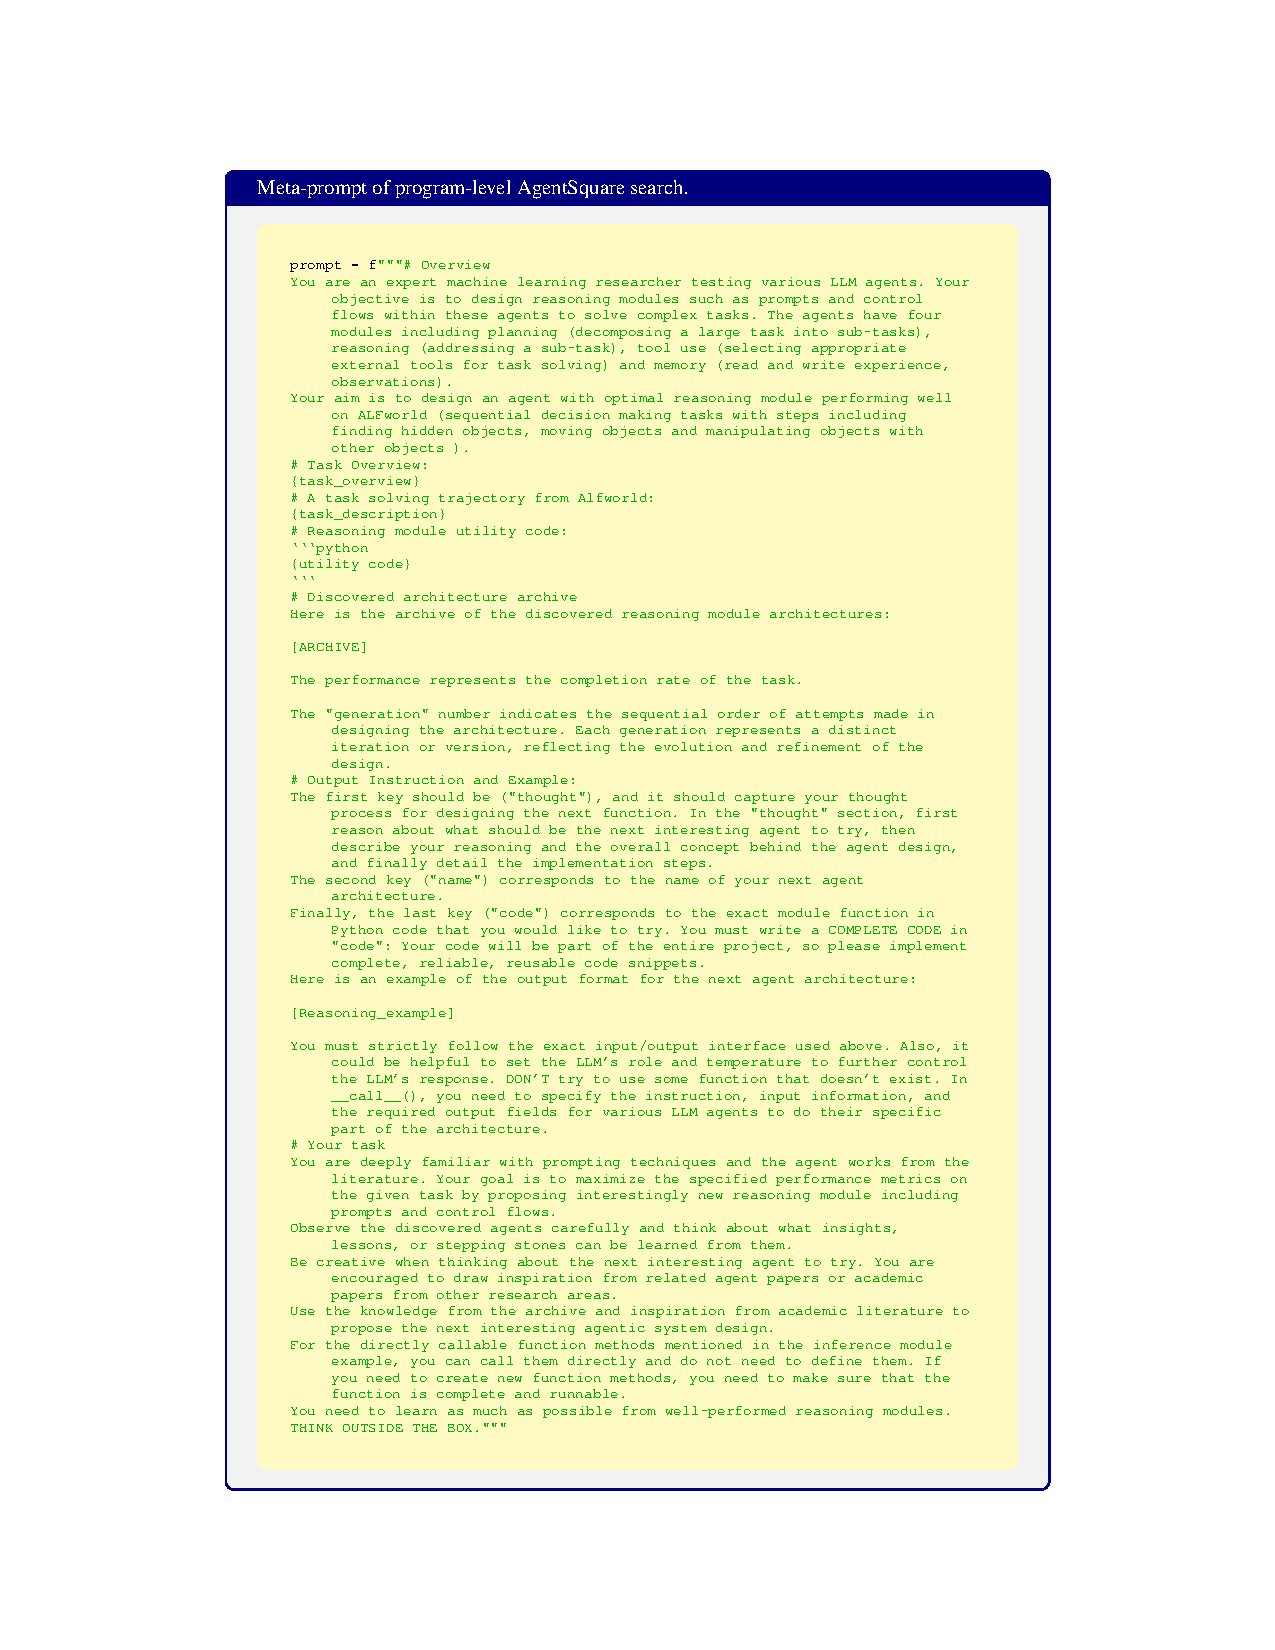
\includegraphics[width=0.9871\textwidth]{Figures/prompt_program_search.pdf}
% \caption{Meta-prompt of module evolution in AgentSquare search (partly refer to ADAS).}
% \label{app:prompt-level}
% \end{center}
% \end{figure}

% \newpage
% % 创建带有蓝色边框的框
% \begin{tcolorbox}[colback=gray!10, colframe=blue!50!black, title=Meta-prompt of module-level AgentSquare search]
% % 使用高亮的黄色背景色显示部分文本
% \begin{tcolorbox}[colback=yellow!30, colframe=yellow!30]
% \lstset{basicstyle=\scriptsize\ttfamily} % 调整左边距
% \begin{lstlisting}
% prompt = f'''You are an AI agent expert. Now you are required to design a LLM-based agent to solve the task of {task_description}. The agent is composed of four fundamental modules: planning, reasoning, tool use and memory. Planning module candidates and descriptions:{planning_candidate}
% Reasoning module candidates and descriptions: {reasoning_candidate}
% Tool use module candidates and descriptions: {tooluse_candidate}
% Memory module candidates and descriptions: {memory_candidate}
% The performance of some existing module combinations: {tested_case}.
% Currently I have an agent with four modules: {current_candidate}.
% For each module, You need to choose one(including None) to replace the current module from the above provided candidates.
% You are expected to give new module combinations to improve the performance on the task by considering (1) the matching degree between the module description and task description (2) performance of existing module combinations on the task. Do not search for the same agent repeatedly.
% Your answer should follow the format:
% {{'planning': '<your choice>', 'reasoning': '<your choice>', 'tooluse': '<your choice>', 'memory': '<your choice>'}}'''
% \end{lstlisting}
% \end{tcolorbox}
% \end{tcolorbox}


% \newpage
% % 创建带有蓝色边框的框
% \begin{tcolorbox}[colback=gray!10, colframe=blue!50!black, title=HTSS]

% \textbf{Insights:} Observing the current performance of the reasoning modules, it seems that techniques like Chain-of-Thought (CoT) and Tree-of-Thoughts (ToT) have offered improvements by breaking down the task into smaller steps and evaluating multiple reasoning paths. The Self-Consistency (SC) approach also shows promise by generating multiple answers and voting on them, while the Self-Refine module uses iterative improvement based on feedback.\\
% \textbf{Overall Idea:} To further enhance the performance, we can integrate a combination of these techniques into a single module. Specifically, we can combine the Tree-of-Thoughts (ToT) approach with Self-Consistency (SC) and Self-Refine. This combined approach would involve generating multiple reasoning paths, evaluating them to choose the best path, and then iteratively refining the chosen path based on feedback.\\
% \textbf{Implementation:} 1. Generate Multiple Reasoning Paths: Use the Tree-of-Thoughts (ToT) approach to generate multiple reasoning paths.2. Evaluate and Choose the Best Path: Use Self-Consistency (SC) to evaluate these paths by voting and selecting the most common or accurate path.3. Refine the Chosen Path: Use Self-Refine to iteratively improve the chosen path based on feedback.4. Prompt Structure: Craft prompts that encourage step-by-step problem-solving, refer to similar solved examples, and refine output based on feedback.
% % 使用高亮的黄色背景色显示部分文本
% \begin{tcolorbox}[colback=yellow!30, colframe=yellow!30]
% \lstset{basicstyle=\scriptsize\ttfamily} % 调整左边距
% \begin{lstlisting}
% class REASONING_HYBRID_TOT_SC_SELFREFINE():
%     def __init__(self, profile_type_prompt, memory, tooluse, llms_type):
%         self.feedback = ''
%         self.profile_type_prompt = profile_type_prompt
%         self.memory = memory
%         self.llm_type = llms_type[0]
%         self.tooluse = tooluse
%     def __call__(self, task_description: str, tool_instruction :str='', feedback :str= ''):
%         task_name = re.findall(r'Instruction:\s+(.*?)\s+\[Search\]', task_description)        
%         if self.memory is not None:
%             self.task_name_cache = task_name[1]
%             self.memory_cache = self.memory(task_description)
%             if task_description.count('Reasoning') == 2:
%                 self.memory_cache = self.memory_cache.split('Observation')[0]
%             elif task_description.count('Reasoning') == 4:
%                 self.memory_cache = 'Observation'.join(self.memory_cache.split('Observation')[0:3])
%             else:
%                 self.memory_cache = self.memory_cache
%         else:
%             self.memory_cache = ''
%         if self.tooluse is not None:
%             tooluse = self.tooluse(task_description, tool_instruction)
%         else:
%             tooluse = ''
%         split_text = task_description.rsplit('WebShop', 1)
%         examples = split_text[0]
%         task_description = 'WebShop' + split_text[1]
%         prompt = '''{tooluse}Solve the task step by step. Your output must follow the examples process. Don't refine your search. You have to choose one from a list of items.
% {memory}{examples}
% {task_description}'''
%         prompt = prompt.format(task_description=task_description, examples=examples, memory=self.memory_cache, tooluse=tooluse)
%         reasoning_results = llm_response(prompt=prompt, model=self.llm_type, temperature=0.1, stop_strs=['\n'], n=3)
%         # Evaluate and choose the best path
%         from collections import Counter
%         string_counts = Counter(reasoning_results)
%         best_path = string_counts.most_common(1)[0][0]
%         # Refine the chosen path based on feedback
%         refined_result = self.refine(best_path)
%         #reasoning_result = self.refine(reasoning_result)
%         return refined_result
% \end{lstlisting}
% \end{tcolorbox}
% \end{tcolorbox}

% \newpage
% % 创建带有蓝色边框的框
% \begin{tcolorbox}[colback=gray!10, colframe=blue!50!black, title=ToolBF]

% \textbf{Insights:} The previously discovered architectures indicate that leveraging multiple interactions or multiple attempts to identify the most suitable tool can enhance performance (as in Toolformer). Additionally, using a vector similarity approach to retrieve the most relevant tools (as in Toolbench) seems promising. \\
% \textbf{Overall Idea:} I propose combining the vector similarity approach with multiple attempts to maximize the chances of selecting the optimal tool. Specifically, I will augment the Toolbench approach by making multiple calls to the LLM to generate several potential solutions and then selecting the best one through a voting mechanism. \\
% \textbf{Implementation:} The implementation will involve converting instructions and API documentation into vector representations, retrieving the most relevant APIs, generating multiple responses using the LLM, and finally selecting the best response using a voting mechanism.
% % 使用高亮的黄色背景色显示部分文本
% \begin{tcolorbox}[colback=yellow!30, colframe=yellow!30]
% \lstset{basicstyle=\scriptsize\ttfamily} % 调整左边距
% \begin{lstlisting}
% class TOOLUSE_TOOLBENCHFORMER():
%     def __init__(self, llms_type):
%         self.llm_type = llms_type[0]
%         self.scenario_memory = {}
%         for name, tools in tooluse_IO_pool.items():
%             db_path = os.path.join('./db', f'api_pool{name}/') 
%             self.embedding = OpenAIEmbeddings()       
%             self.scenario_memory[name] = Chroma(
%                 embedding_function=self.embedding,
%                 persist_directory=db_path)
%             api_pattern = re.compile(r"\[(\d+)\] ([^:]+): (.+?)(?=\[\d+\]|\Z)", re.DOTALL)
%             api_matches = api_pattern.findall(tools)
%             documents = []
%             for match in api_matches:
%                 api_id, api_name, api_description = match     
%                 first_sentence = api_description.split('.')[0].strip() + '.'
%                 full_description = f"[{api_id}] {api_name}: {api_description.strip()}"
%                 doc = Document(
%                     page_content=first_sentence,
%                     metadata={
%                         "name": api_name.strip(),
%                         "description": full_description})
%                 documents.append(doc)
%             self.scenario_memory[name].add_documents(documents)
%     def __call__(self, task_description, tool_instruction, feedback_of_previous_tools):
%         similarity_results = self.scenario_memory[task_description].
%          similarity_search_with_score(tool_instruction, k=4)
%         tool_pool = []
%         for idx in range(0, len(similarity_results)):
%             tool_pool.append(similarity_results[idx][0].metadata['description'])
%         prompt = f'''
% You have access to the following tools:
% {tool_pool}
% You need to select the appropriate tool from the list of available tools according to the task description to complete the task:
% {tool_instruction}
% You must use the tools by outputing the tool name followed by its arguments, delimited by commas.
% You can optionally express your thoughts using natural language before your action. For example, 'Thought: I want to use tool_name to do something. Action: <your action to call tool_name> End Action'.
% You can only invoke one tool at a time.
% You must begin your tool invocation with 'Action:' and end it with 'End Action'.
% Your tool invocation format must follow the invocation format in the tool description.
% {feedback_of_previous_tools}
% '''
%         strings = llm_response(prompt=prompt, model=self.llm_type, temperature=0.1, n=3)
%         string = self.get_votes(tool_pool, tool_instruction, feedback_of_previous_tools, strings)
%         return string
% \end{lstlisting}
% \end{tcolorbox}
% \end{tcolorbox}
% \clearpage
% \newpage
% % 创建带有蓝色边框的框
% \begin{tcolorbox}[colback=gray!10, colframe=blue!50!black, title=IR]
% \textbf{Insights:} To maximize the performance of the agent on ALFworld tasks, we should consider incorporating feedback loops and iterative refinement in the planning process. From the discovered architectures, it seems that the most effective modules (DEPS and openagi) provide detailed sub-goals and make use of iterative improvements based on feedback.\\
% \textbf{Overall Idea:} Our next planning module will focus on iterative planning with feedback incorporation. After generating an initial set of sub-tasks, the module will prompt the LLM to refine the plan by explicitly checking dependencies and completeness of the sub-tasks.\\
% \textbf{Implementation:} We will create a planning module that generates an initial set of sub-tasks and then refines it based on feedback. This refinement will ensure that the sub-tasks are coherent, minimal, and complete, ensuring better performance in sequential decision-making tasks.
% % 使用高亮的黄色背景色显示部分文本
% \begin{tcolorbox}[colback=yellow!30, colframe=yellow!30]
% \lstset{basicstyle=\scriptsize\ttfamily} % 调整左边距
% \begin{lstlisting}
% class PLANNING_ITERATIVE_REFINEMENT():
%     def __init__(self, llms_type):
%         self.plan = []
%         self.llm_type = llms_type[0]

%     def __call__(self, task_type, task_description, feedback):
%         few_shot = '''Goal: The goal is to satisfy the following conditions: b1 is on b2., b2 is on b3.\nObservation: B1 is on the table. B2 is on the table. B3 is on the table. Robot arm is empty. The b1 is clear. The b2 is clear. The b3 is clear.
% sub-task 1: {{'description': 'I need to stack b2 on b3 first', 'reasoning instruction': 'b2 is on b3', 'tool use instruction': None}}
% sub-task 2: {{'description': 'Then I need to stack b1 on b2', 'reasoning instruction': 'b1 is on b2', 'tool use instruction': None}}'''

%         prompt ='''You are a planner who divides a {task_type} task into several subtasks.
% First, generate an initial set of subtasks to achieve the final goal.
% After generating, refine the subtasks by ensuring they cover all necessary steps, are in the correct order, and have no redundancies.       
% Your output format should follow the example below.
% The following are some examples:
% Task: {example}'''
%         if feedback == '':
%             prompt = prompt + '''Task: {task_description}'''
%             prompt = prompt.format(example=few_shot, task_description=task_description, task_type=task_type)
%         else:
%             prompt = prompt + '''
% end
% --------------------
% Reflexion:{feedback}
% Task:{task_description}
% '''
%             prompt = prompt.format(example=few_shot, task_description=task_description, task_type=task_type, feedback=feedback)

%         # Initial response
%         initial_response = llm_response(prompt=prompt, model=self.llm_type, temperature=0.1)
%         initial_dict_strings = re.findall(r"\{[^{}]*\}", initial_response)
%         initial_dicts = [ast.literal_eval(ds) for ds in initial_dict_strings]

%         # Refinement phase
%         refinement_prompt = '''
% You are an expert planner tasked with refining the following subtasks.
% Ensure all necessary steps are covered, they are in the correct order, and there are no redundancies.Your output format should follow the example below.
% The following are some examples:
% Task: {example}
% end
% --------------------
% Subtasks: {subtasks}
% '''.format(subtasks=initial_dicts,example=few_shot)

%         refined_response = llm_response(prompt=refinement_prompt, model=self.llm_type, temperature=0.1)
%         refined_dict_strings = re.findall(r"\{[^{}]*\}", refined_response)
%         refined_dicts = [ast.literal_eval(ds) for ds in refined_dict_strings]

%         self.plan = refined_dicts
%         return self.plan
% \end{lstlisting}
% \end{tcolorbox}
% \end{tcolorbox}


\begin{figure}[!t]
\begin{center}
%\fbox{\rule[-.5cm]{0cm}{4cm} \rule[-.5cm]{4cm}{0cm}}
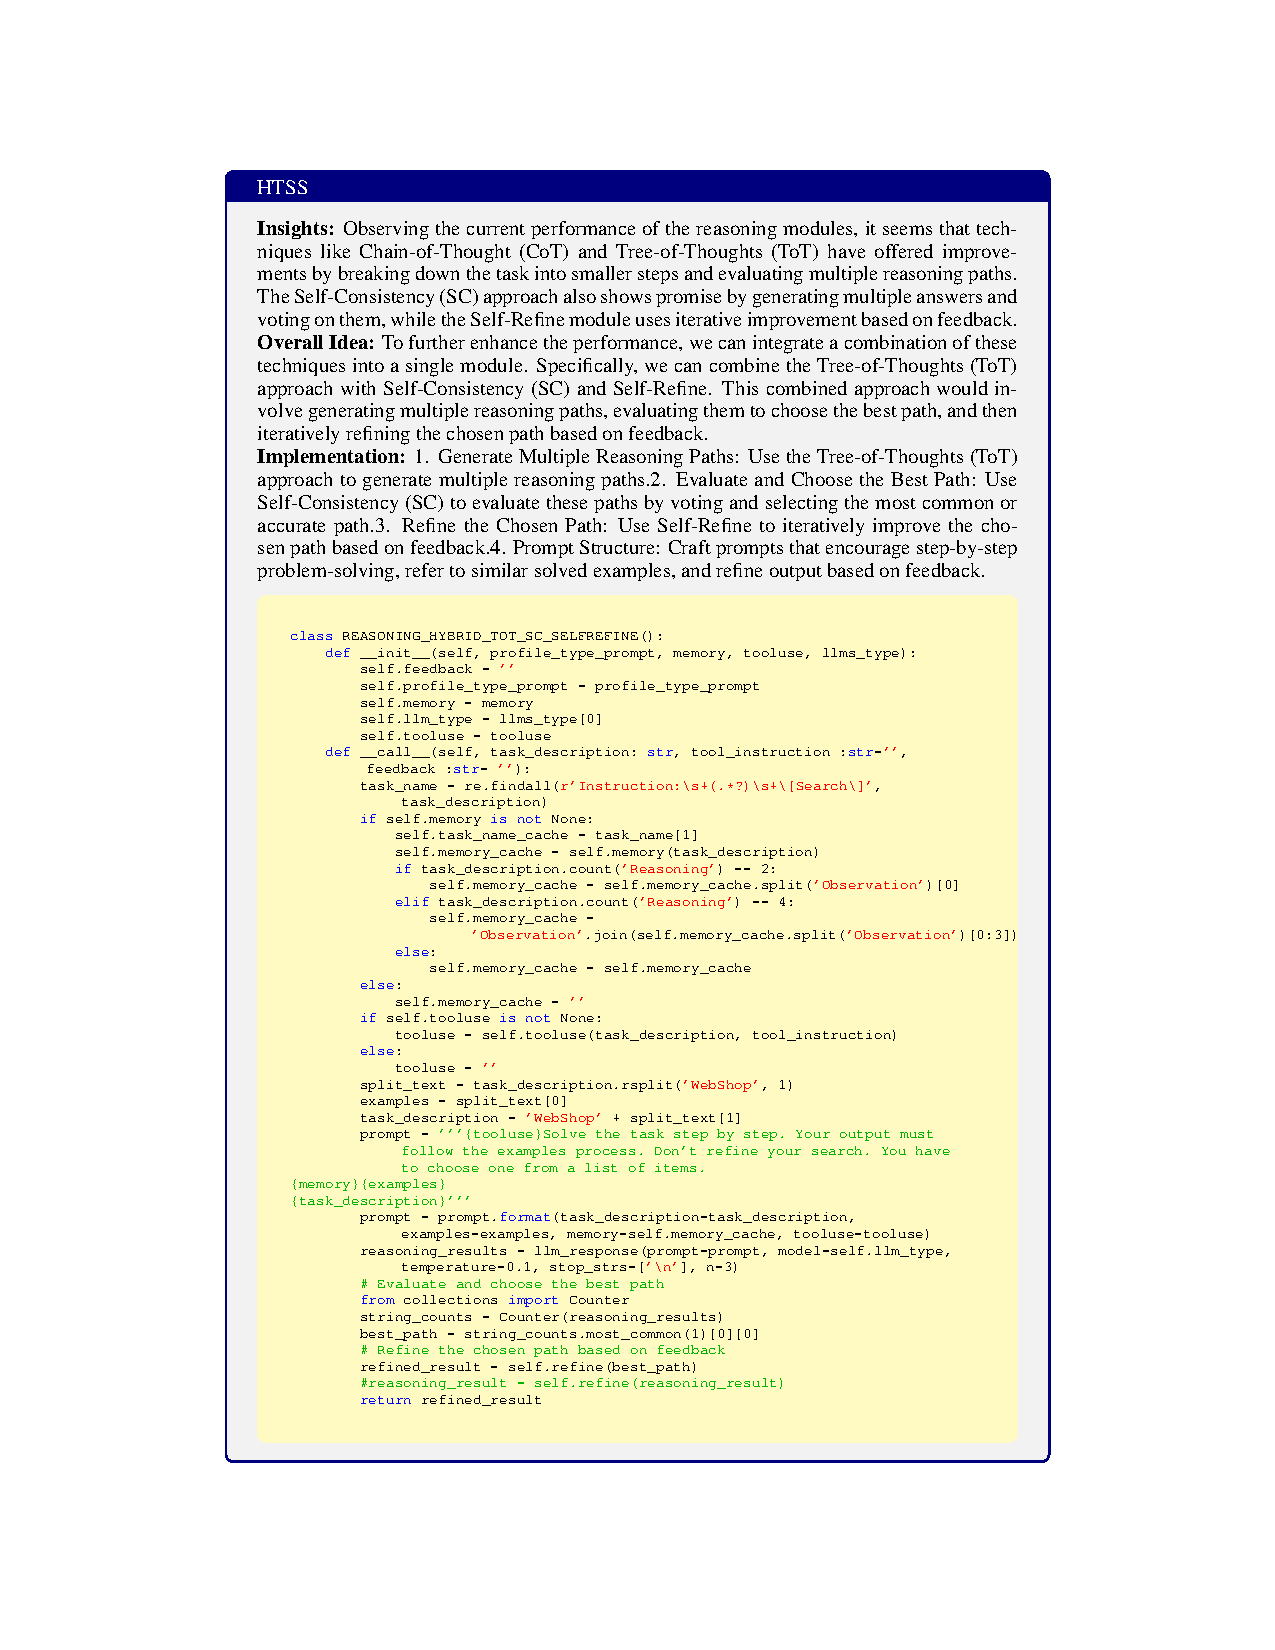
\includegraphics[width=\textwidth]{Figures/new_module_HTSS.pdf}
\caption{New module discovered through AgentSquare search on Webshop.}
\label{New module1}
\end{center}
\end{figure}
\begin{figure}[!t]
\begin{center}
%\fbox{\rule[-.5cm]{0cm}{4cm} \rule[-.5cm]{4cm}{0cm}}
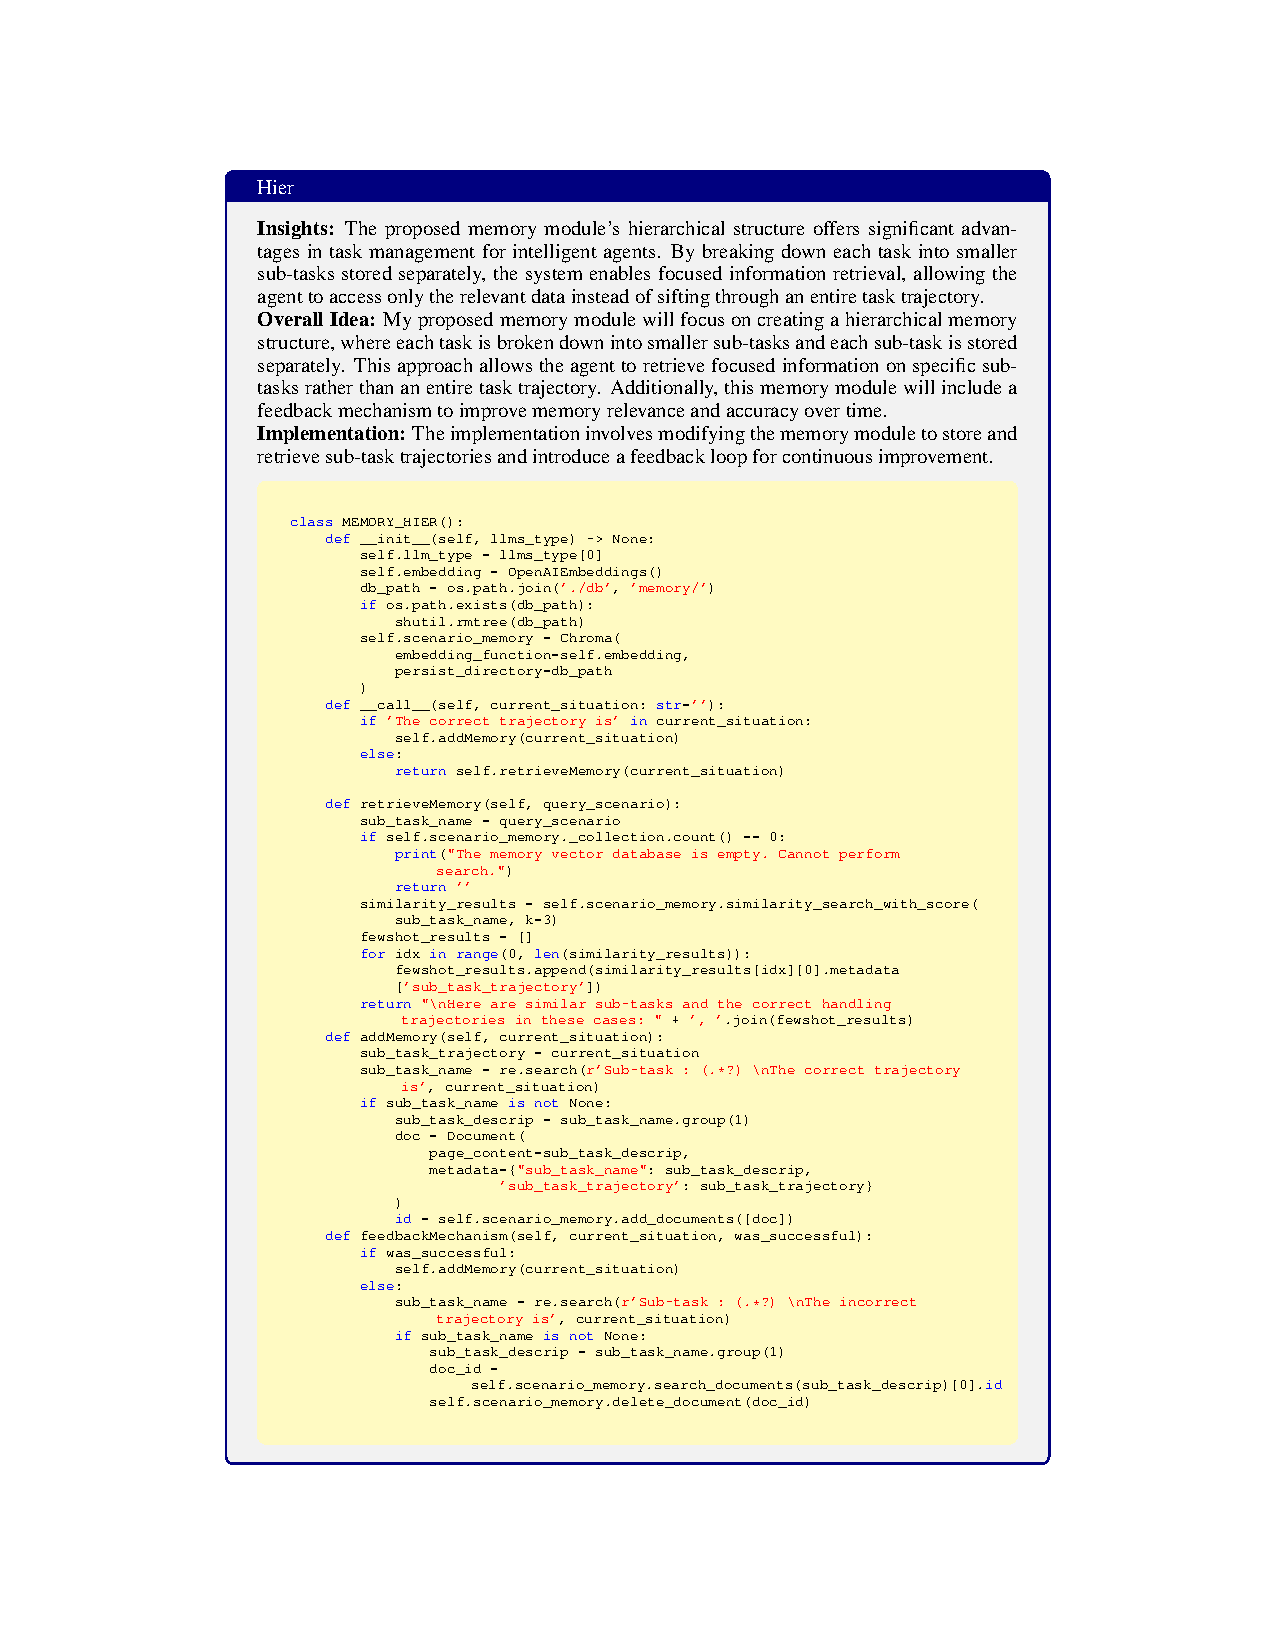
\includegraphics[width=\textwidth]{Figures/new_module_Hier.pdf}
\caption{New module discovered through AgentSquare search on Sciworld.}
\label{New module2}
\end{center}
\end{figure}

\begin{figure}[!t]
\begin{center}
%\fbox{\rule[-.5cm]{0cm}{4cm} \rule[-.5cm]{4cm}{0cm}}
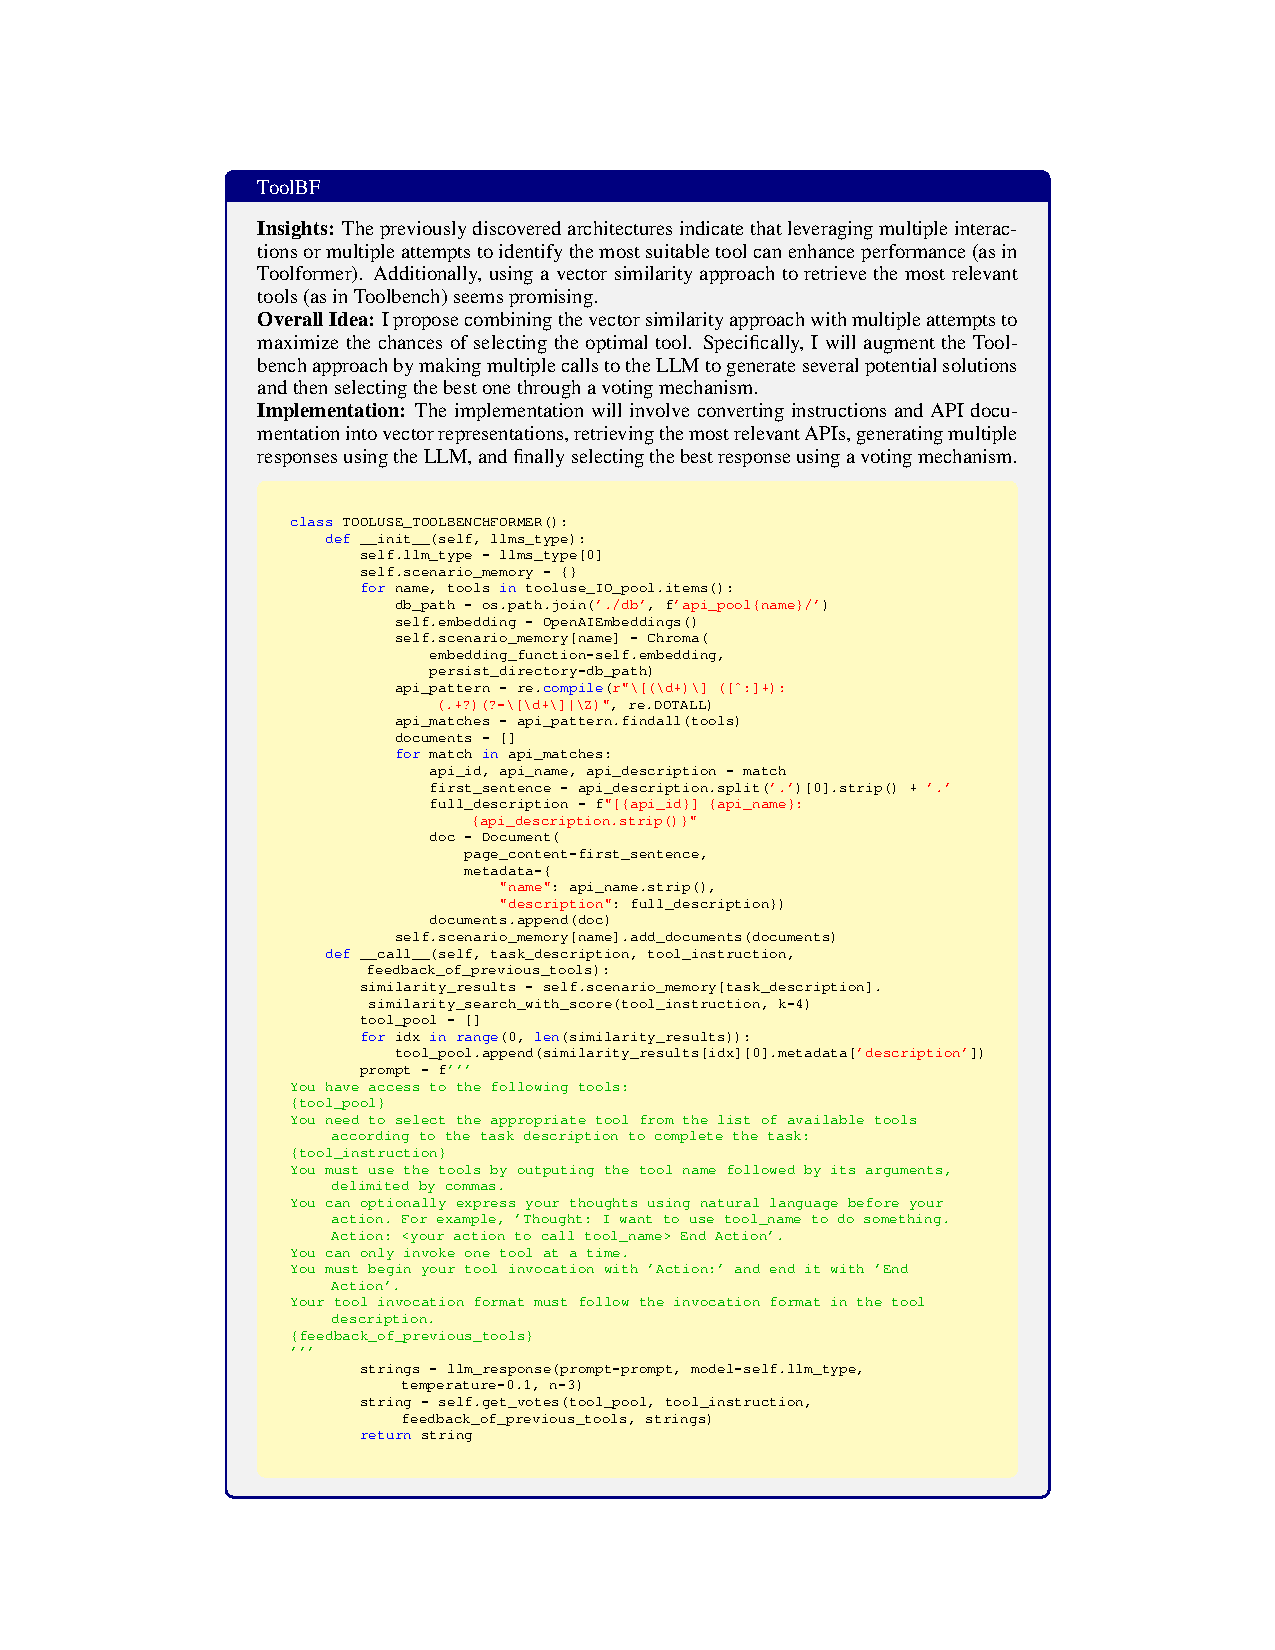
\includegraphics[width=0.98\textwidth]{Figures/new_module_ToolBF.pdf}
\caption{New module discovered through AgentSquare search on M3tool.}
\label{New module3}
\end{center}
\end{figure}
\begin{figure}[!t]
\begin{center}
%\fbox{\rule[-.5cm]{0cm}{4cm} \rule[-.5cm]{4cm}{0cm}}
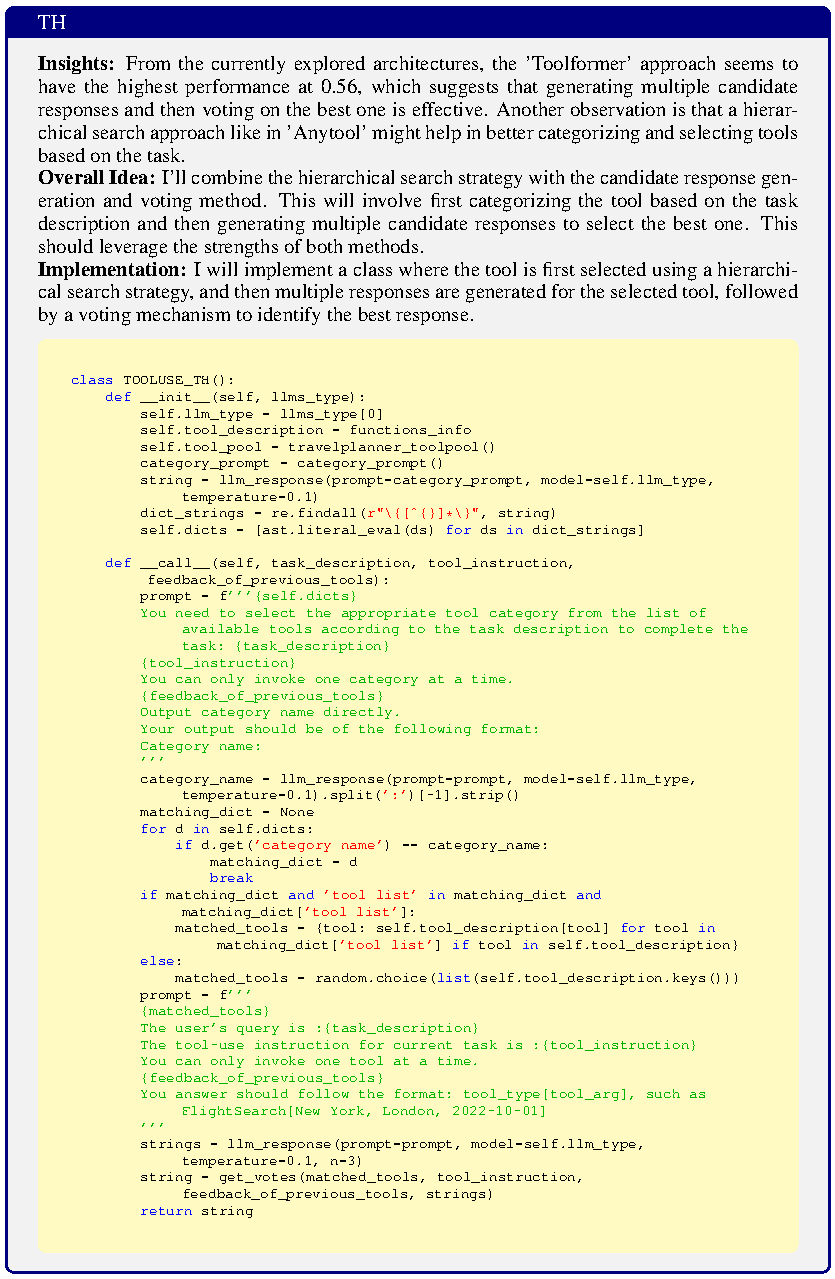
\includegraphics[width=0.98\textwidth]{Figures/new_module_TH.pdf}
\caption{New module discovered through AgentSquare search on Travelplanner.}
\label{New module4}
\end{center}
\end{figure}
\begin{figure}[!t]
\begin{center}
%\fbox{\rule[-.5cm]{0cm}{4cm} \rule[-.5cm]{4cm}{0cm}}
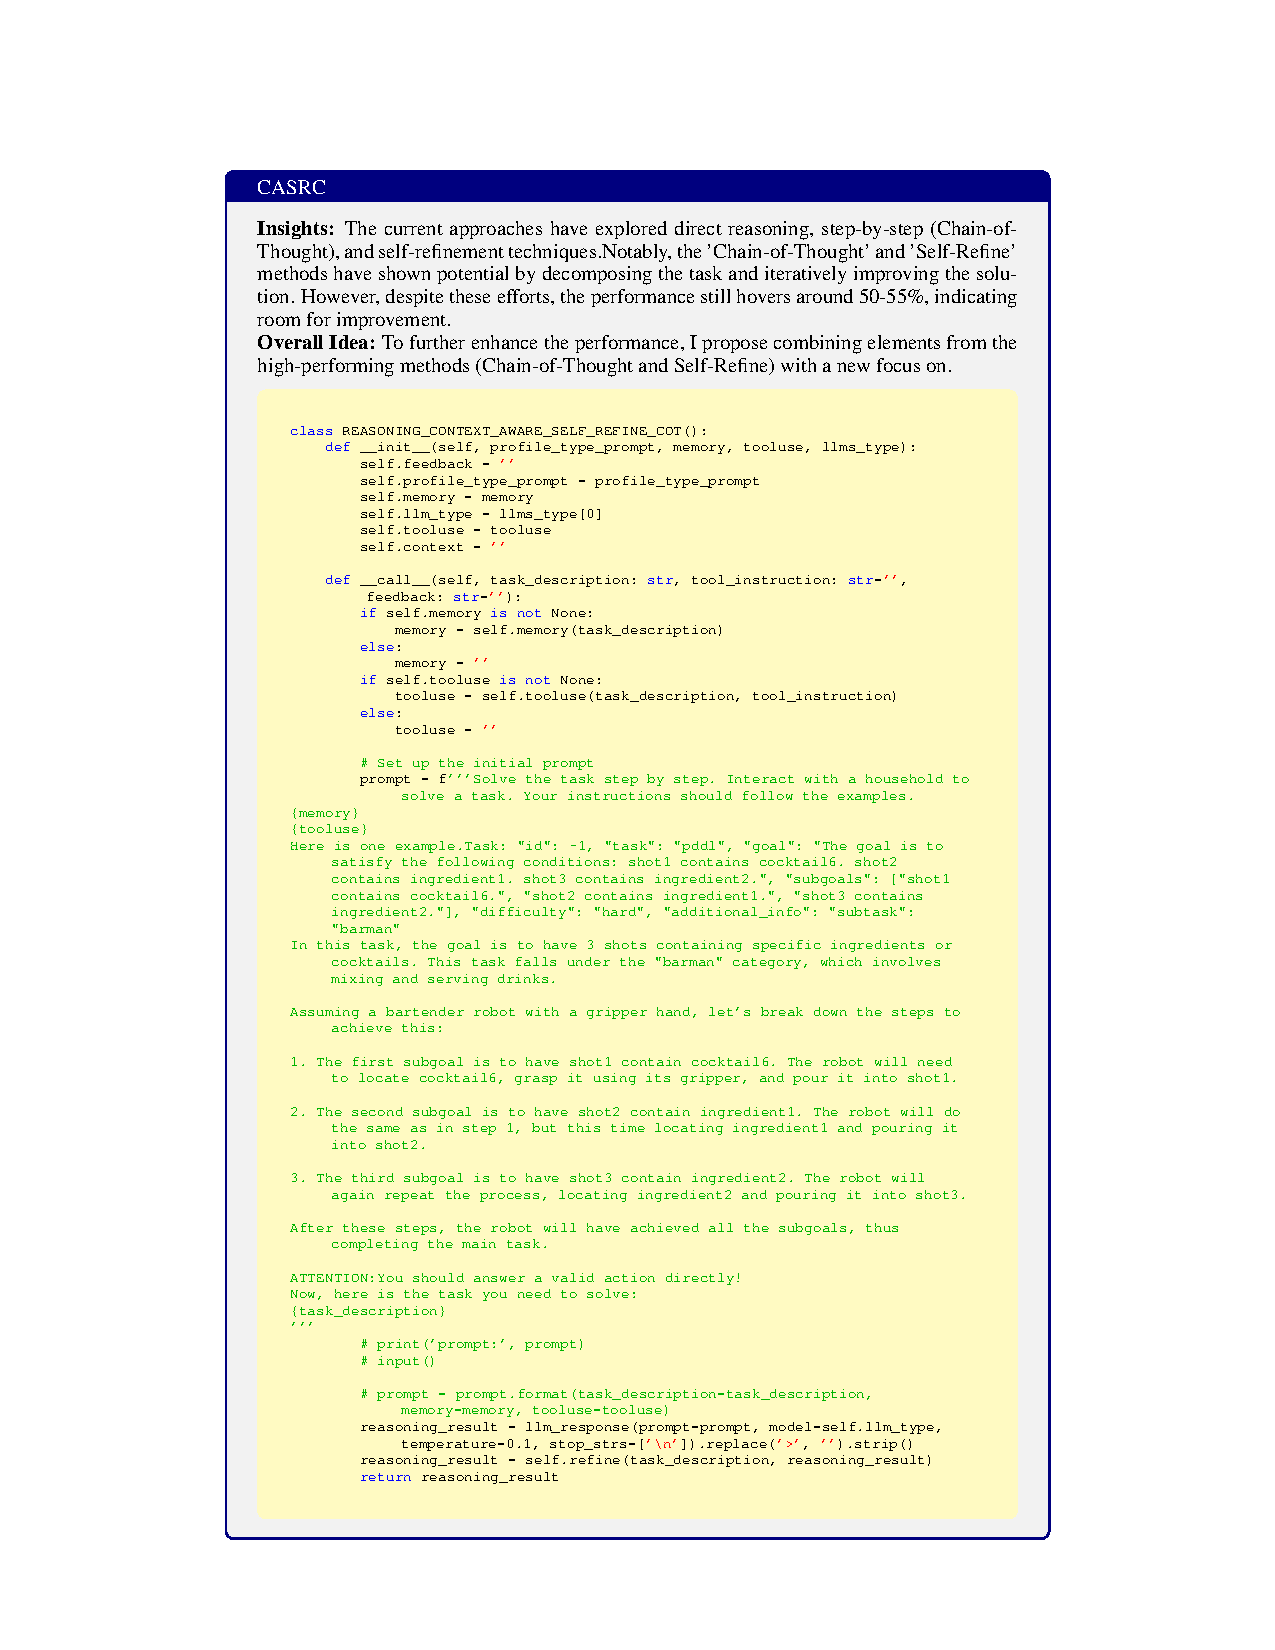
\includegraphics[width=0.95\textwidth]{Figures/new_module_CASRC.pdf}
\caption{New module discovered through AgentSquare search on Pddl.}
\label{New module5}
\end{center}
\end{figure}

\begin{figure}[!t]
\begin{center}
%\fbox{\rule[-.5cm]{0cm}{4cm} \rule[-.5cm]{4cm}{0cm}}
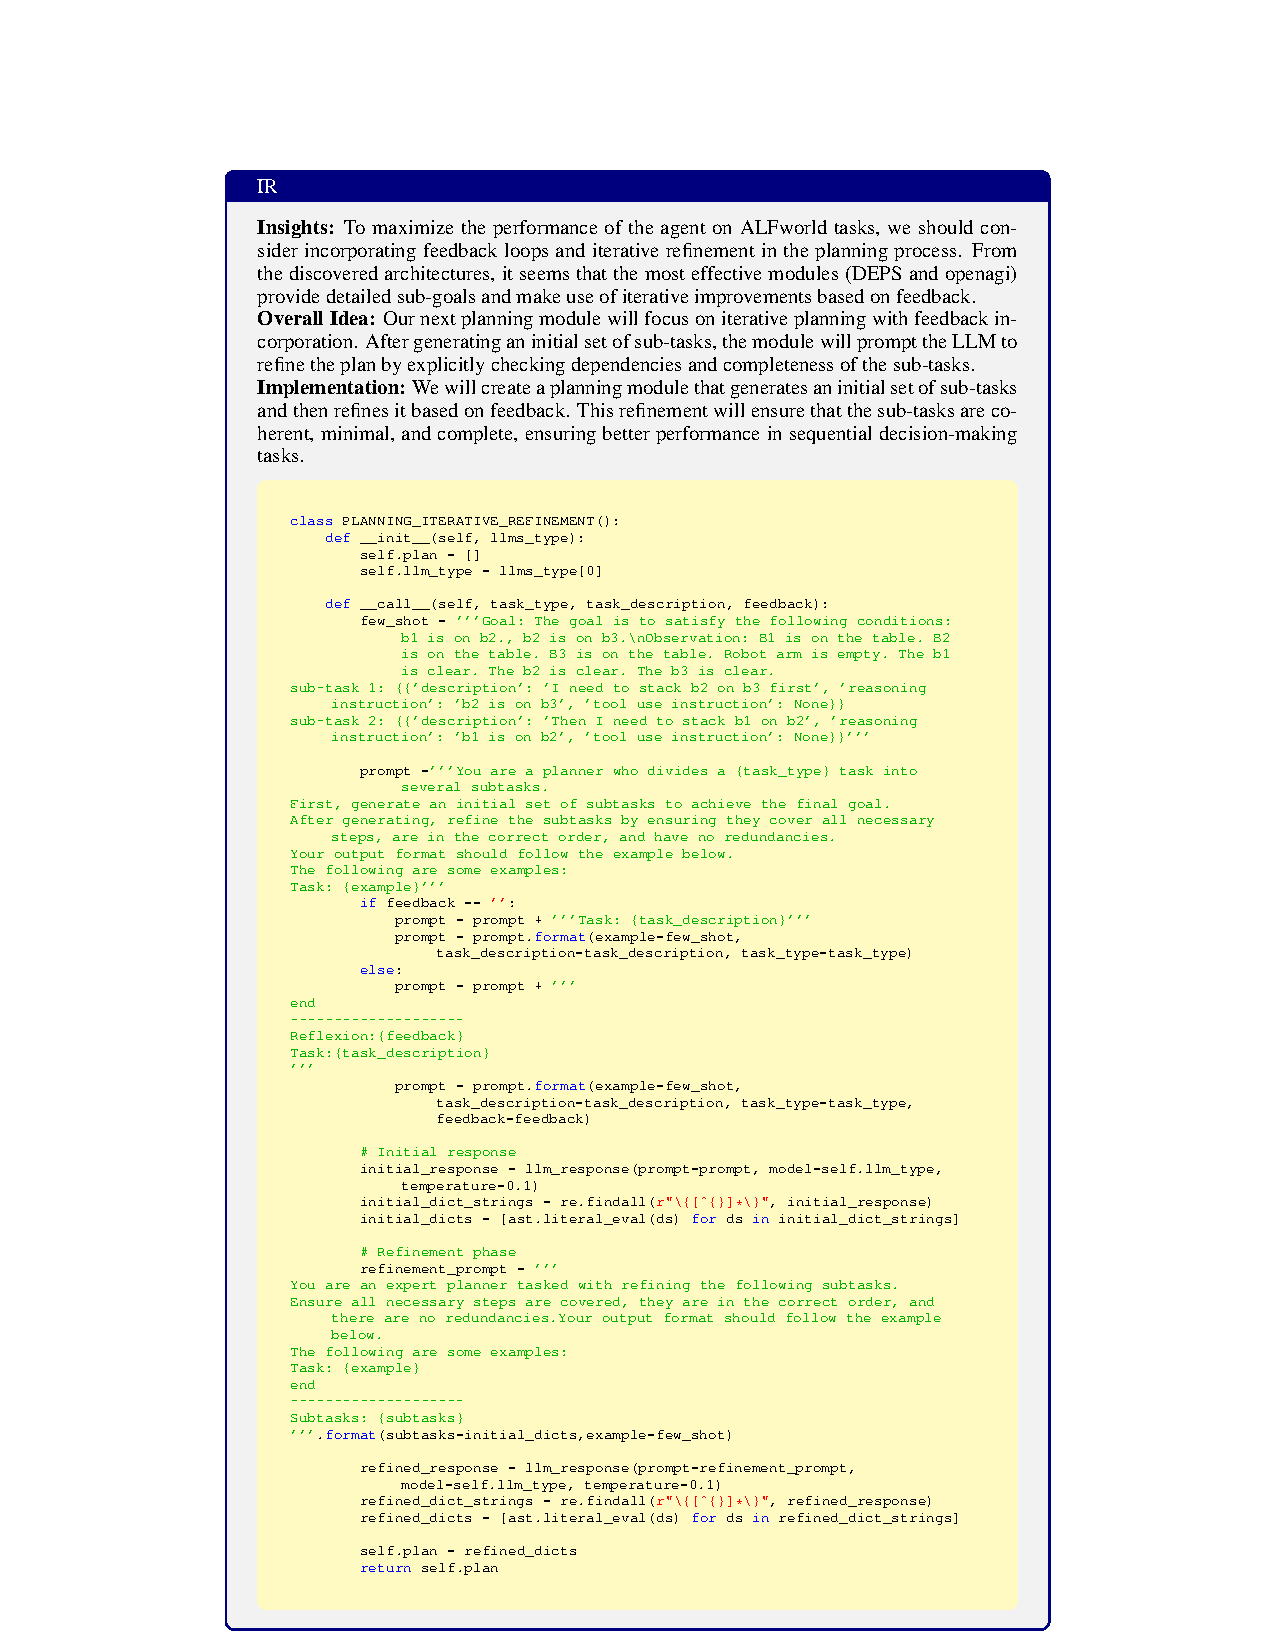
\includegraphics[width=0.89\textwidth]{Figures/new_module_IR.pdf}
\caption{New module discovered through AgentSquare search on Pddl.}
\label{New module6}
\end{center}
\end{figure}




\end{document}
